%
% File: thesisexample.tex   Version 1.8   May 6, 1999
%
% This is an example document for easychithesis, a 
% LaTeX2e style for formating theses at the University of
% Chicago.The easychithesis style was written by Bryan Clair and 
% Nathan Dunfield.  It contains detailed instructions for using
% easychithesis.
%
%  HINTS:
%
%  1. To get appendices, you don't do anything different from a normal
%     report document.  That means, put the command \appendix before
%     you begin your first appendix, then do each appendix with a
%     \chapter command.  Note that if you have only one appendix, it is
%     customary to leave it unnumbered.  Do this with \chapter*.
%
%  2.  If you use \chapter*, which produces unnumbered chapters, you 
%       have to add that chapter to the table of contents by hand, e.g.
%
%         \chapter*{Appendix}
%         \addcontentsline{toc}{chapter}{Appendix}
%
%  3.  If you get errors about
%   
%    Undefined control sequence.
%         \setspace@size ...rrsize \normalsize \@normalsize \else \@currsize \fi 
%
%     You need a newer version of the file ``setspace.sty''.
%
%  4.  Problems with math formulas in chapter headings:
% 
%         a.  Any lowercase letters in the formula are converted to
%         uppercase, e.g. f(x) becomes F(X).   If you really need
%         lowercase math letters in your chapter titles, use the
%         option plainchapterheads (and, if you want, type your
%         chapter titles in ALL CAPS so that the appearance doesn't
%         change).  Note there is no problem 
%         for section or subsection headings in either case.  (Options
%         such as plainchapterheads are given as part of the 
%         \documentclass command, see below under ``Document Options'').
%
%         b.  Some perfectly reasonable math commands when used in
%         \chapter give the error
%          ``LATEX ERROR: \command  ALLOWED ONLY IN MATH MODE.''
%         The solution to this is to do
%        
%              \newcommand{\mymath}{problem math goes here}
%       
%         and then
%        
%              \chapter{All about \protect\mymath}
%
%         also, the option plainchapterheads will fix this too.
%
%  5. If your References section doesn't show up in the table of
%     contents, you need to add the line \addcontentsline...
%     as done at end of this file.   Make sure that you include the 
%     page break command as done there or else you may end up
%     with the wrong page number in your table of contents. 

\documentclass{ucetd}
% Document Options: 
%
% Note if you want to save paper when printing drafts, replace the
% above line by
% 
%   \documentclass[singlespace]{easychithesis}
% 
% or 
% 
%   \documentclass[onehalfspace]{easychithesis}
%
% Also the ``double spacing'' provided by this style is not ``true''
% doublespacing as defined by setspace.sty.  Instead, it is the same
% as on the old LaTeX 2.09 thesis style ``chithesis''.  If you want 
% ``true'' doublespacing (if there is such a thing), give the option 
% truedoublespace.  The increase in tree murder will be on your 
% conscience, not mine.
%
%  Similarly, if you need to use the plainchapterheads option, you do
%   
%  \documentclass[plainchapterheads]{easychithesis}
%
% You can give more than one option, if you desire.
\usepackage{pdfpages}
\usepackage{csquotes}
\usepackage{nameref}
\usepackage{amsmath}    % need for subequations
\usepackage{graphicx}   % need for figures
\usepackage{changepage}
\usepackage{float}
\usepackage{caption}
\captionsetup{font={stretch=1}}
\usepackage{rotating}
\usepackage{subfigure,epsfig,amsfonts}
\usepackage{natbib}

\usepackage{amssymb}
\usepackage{amsthm}
%\usepackage{verbatim}   % useful for program listings
%\usepackage{color}      % use if color is used in text
%\usepackage{subfigure}  % use for side-by-side figures
%\usepackage{hyperref}   % use for hypertext links, including those to external documents and URLs
\usepackage[numbered,framed]{docu/matlab-prettifier}

\let\ph\mlplaceholder % shorter macro
\lstMakeShortInline"

\lstset{
	style              = Matlab-editor,
	basicstyle         = \mlttfamily,
	escapechar         = ",
	mlshowsectionrules = true,
}
\begin{document}

% Create the official title
\title{Dynamic modulation of actomyosin contractility and cortical flow by actin filament recycling} 
\author{William McFadden}
\date{June 2017}
\department{Biophysical Sciences}
\degree{Doctor  of Philosophy} 

% \dedication : Use for a dedication, copyright, or epigraph.
%               Produces a page with no number for the text which follows
%               If you want centering, do it yourself with 
%               \begin{center} and \end{center}.  You can have more
%               than one `dedication'.
\dedication{ For Claire, you kept me going.}




 

%% Basic setup commands
% If you don't want a title page comment out the next line and uncomment the line after it:
\maketitle
%\omittitle

% These lines can be commented out to disable the copyright/dedication/epigraph pages
\makecopyright
\makededication


%% Make the various tables of contents
\tableofcontents
\listoffigures
\listoftables

\acknowledgments
I'd like to thank my advisor, Ed Munro, Birali Runesha, Francois Robin, Patrick McCall, Jon Michaux, Younan Li, Baixue Yao, Shiladitya Banerjee, the University of Chicago Biophysical Sciences program, Michele Wittels, Artifice, Pete Dahlberg, Adam Hammond, James Crooks, the uchicago myCHOICE program, the Insight Data Science Fellowship Program, Color Genomics, Robbie Sliwinski, my fiancee, Claire Stevenson, her family, David Stevenson and Marilyn Lucas, my brother, Andrew McFadden, and my mom, Deb McFadden.  Without all of these people and programs, I wouldn't have made it through this work and come out the other side with something of value.


\abstract
Actomyosin-based cortical flow is a fundamental engine for cellular morphogenesis.  Cortical flows are generated by cross-linked networks of actin filaments and myosin motors, in which active stress produced by motor activity is opposed by passive resistance to network deformation.  Continuous flow requires local remodeling through crosslink unbinding and/or filament disassembly. But how local remodeling tunes stress production and dissipation, and how this in turn shapes long range flow, remains poorly understood. To address this question, I developed a computational model for cross-linked actomyosin networks based on minimal requirements for production and dissipation of contractile stress, namely asymmetric filament compliance, spatial heterogeneity of motor activity, reversible cross-links and filament turnover.  Using this model, I characterized systematically how the production and dissipation of network stress each depend on network architecture, cross-link dynamics and filament turnover.  Then I determined how these dependencies combine to determine overall rates of cortical flow. My analysis predicts that filament turnover plays two key roles in shaping cortical flow: First, it allows networks to maintain active stress at steady state against external resistance and second,  it allows networks to continuously dissipate passive internal resistance to external force, while maintaining structural integrity. My model predicts that steady state stress increases with filament lifetime up to a characteristic time $\tau_{a}$, then decreases with lifetime above $\tau_{a}$; Effective viscosity increases with filament lifetime up to a characteristic time $\tau_c$, and then becomes independent of filament lifetime and sharply dependent on crosslink dynamics.  Finally, I show that these individual dependencies of active stress and effective viscosity define multiple regimes of steady state flow.  In particular my model predicts the existence of a regime, where filament lifetimes are shorter than both $\tau_c$ and $\tau_{a}$, in which dependencies of effective viscosity and steady state stress cancel one another, such that flow speed is insensitive to filament turnover.  My model also predicts a simple dependence of flow velocity on molecular scale properties of motor activity and crosslink dynamics.  In complementary work, in collaboration with other members of the Munro Lab, I developed methods to measure actin filament turnover in C. elegans embryos using single molecule imaging. Together, these results provide a framework for understanding how animal cells tune cortical flow through local control of network remodeling.  

\mainmatter

%
% Body Chapters
%
\chapter{Introduction}

\section{Biological Context of Cortical Flow}
Many essential cellular processes, including cell polarization, cytokinesis and cell migration, depend on the fundamental ability of cells to undergo rapid and dynamic internal remodeling \cite{bhl28884}. To remodel themselves, cells must be able to reorganize a complex array of organelles and cytoskeletal machinery in a highly coordinated manner, while maintaining structural integrity.  How they achieve this remains a key open question in the field of cell biology.

One fundamental and ubiquitous form of cellular remodeling is known as cortical flow.  Cortical flows originate within a thin layer of cross-linked actin filaments and myosin motors, called the actomyosin cortex, that lies just beneath the plasma membrane \cite{Munro2004413}. Cortical flows are characterized by long range fluid-like movements of cortical material over distances comparable to the length of the cell \cite{doi:10.1146/annurev-cellbio-100109-104027}.  Cortical flows are thought to be driven by spatial gradients of stress originating from spatial variation in myosin motor activity, which leads to movements of cortical material from regions of low stress to regions of high stress \cite{cellmech_flows3}.

Cortical flow plays an essential role in a wide variety of biological processes, including  cell polarization, cell division, cell crawling and multicellular tissue morphogenesis \cite{cellmech_flows3, cellmech_flows2, Benink:2000aa, Wilson:2010aa, Rauzi2010, Munro2004413}. For example, cortical flow drives the segregation of conserved  “polarity determinants,” known as PAR proteins, to establish the primary embryonic axis of the single-cell \textit{C. elegans} embryo \cite{Munro2004413,Goehring1208619}. Before polarization, the PAR proteins PAR-3, PAR-6 and PKC-3 are distributed evenly around the cortex of the cell. However to establish the anterio-posterior axis, these proteins must become enriched at the anterior cortex. Cortical flow generates this asymmetry by actively transporting PAR-3, PAR-6 and PKC-3 to the anterior pole. An asymmetric flow is generated from the sperm entry point, which occurs at the nascent posterior pole of the embryo and causes a local decrease in an upstream regulator of myosin contractility \cite{Munro2004413,motegi}. This small asymmetry leads to a gradient in myosin activity across the embryo, resulting in a gradient of contractile stress  \cite{cellmech_flows, cellmech_flows3} that drives cortical flows towards the anterior pole. Cortical flows also play an important role in amoeboid motility. Recent work in a variety of different amoeboid cell types has shown that during migration there is a rapid flow of actin and myosin toward the rear of the cell \cite{amoeba1, amoeba2, amoeba3, amoeba4, Yumura200}. It is thought that this flow can propel the cell forward by exerting traction on external substrates, either through focal adhesions, as in mesenchymal cells, or through non-specific frictional coupling as in most other amoeboid cells \cite{amoeba1}. Finally, cortical flows can also contribute to tissue-level morphogenetic movements \cite{Salbreux2012536,Munjal1789}.  For example, during epiboly in the zebrafish embryo, the enveloping cell layer, an epithelial monolayer of cells on the outer surface of the embryo, spreads around the yolk \cite{epib_review}.  The small region of yolk just beyond the spreading cells, known as the yolk syncytial layer, is enriched in actomyosin, which appears to flow in a direction opposite to the direction of cell spreading. This actomyosin flow is thought to exert forces against the underlying yolk cytoplasm through a flow-friction mechanism similar to that proposed for amoeboid movement \cite{Behrndt257}. These and other examples highlight how the same core mechanism---actomyosin-based cortical flow---can contribute to a variety of cellular processes in a diversity of different species. Understanding how cortical flows arise and how they are regulated is key to advancing our understanding of the role of cortical flows in these processes.

To understand how the actomyosin cortex gives rise to cortical flows, it is essential to synthesize knowledge across two distinct scales of description: a microscopic description in terms of the molecular components and their interactions, and a macroscopic, continuum-level, description in terms of active forces, passive resistance and flow velocity. Over the last few decades, molecular studies have generated a wealth of knowledge about the molecular players - e.g. actin and myosin and crosslinkers - and their interactions. At the same time, physicists have constructed macroscopic theoretical descriptions of the cortex as a kind of active fluid \cite{cellmech_flows}. However, it remains a fundamental challenge to bridge the gap between the properties of the molecular elements and quantities like stress and viscosity, which appear in the theoretical models.  

The overarching goal of my research is to understand how the  macroscopic dynamics of cortical flow arise from and are controlled by microscopic properties and interactions. To accomplish this, I set out to build a molecular scale model based on empirical properties of actin filaments, cross-linking proteins and myosin motor complexes, that could be used to predict the macroscopic dynamics of cortical flow. Specifically, the model must  be capable of generating continuous flow in response to a spatial gradient of motor activity. I explicitly limit the complexity of the molecular model to facilitate direct comparisons with the predictions of the macroscopic theory. To do so, I will be making a number of key simplifying assumptions, which aim to balance the realistic behavior of cytoskeletal mechanics with a tractable simplified model. This work will allow me to shed new light on the molecular players that contribute to the physics underlying cortical flows. This avenue of study is not only important for understanding the biological functions of cortical flow, but it is also a fundamental challenge in soft matter physics that goes beyond biology.


\section{Introduction to the Cortical Actomyosin Cytoskeleton}
\label{sec:basic}
Decades of research have revealed a great deal about the cytoskeletal machinery that operates within cells to  drive cortical flows. The cortical actomyosin cytoskeleton is a thin meshwork of actin filaments that are interconnected by cross-linking proteins and ensembles of myosin motors known as myosin mini-filaments \cite{Alberts}.  The cortex  is continuously renewed through cycles of actin filament polymerization/depolymerization, crosslink binding/unbinding and myosin mini-filament assembly/disassembly \cite{phys_bio_cell}. The cortical cytoskeleton  provides structural support to the cell, and also generates and transduces the mechanical forces that carry out essential functions such as cellular shape change and migration.  In the following sections, I will highlight the key structural components and biochemistry of the actomyosin cortex that enables it to undergo cortical flows.

\paragraph{Actin Filaments} Actin filaments are polar semi-flexible polymers composed of chains of actin monomers that are held together by reversible supramolecular bonds.  Actin monomers can spontaneously polymerize in solution or they can be actively nucleated and/or elongated in vivo by factors such as formins, which give rise to long linear filaments, or the ARP2/3 complex, which gives rise to shorter branched networks such as those found in lamellipodia \cite{phys_bio_cell}.  Addition of monomers to the actin filament occurs preferentially at one end of the filament known as the barbed (plus) end due to the difference in binding constants between ATP and ADP bound forms of actin monomers \cite{doi:10.1146/annurev-biophys-051309-103849}. The barbed end contains an abundance of ATP bound actin compared to the opposite end, known as the pointed (minus) end, which has a greater abundance of ADP bound actin. The binding affinity between ATP bound actin monomers is greater than that between ADP bound monomers, thus polymerization preferentially occurs at the barbed end and disassembly preferentially occurs from the pointed end.  Assembly and disassembly from opposite ends of a filament causes a phenomenon known as actin treadmilling. During treadmilling, filaments are depolymerized from their minus ends as they grow from the plus end, which causes the filament to apparently translocate while turning over \cite{doi:10.1146/annurev-biophys-051309-103849}.  Turnover can also be enhanced by regulators of depolymerization including cofilin and gelsolin \cite{bemenet}. These factors can sever filaments internally, creating new minus ends with ADP bound actin, which leads to a rapid depolymerization of the exposed ends.  Experimental studies \textit{in vivo} reveal that these mechanisms of depolymerization can result in rapid turnover of cortical actin filaments on timescales of 5 to 100 seconds, much faster than would occur through actin treadmilling alone \cite{Robin:2014aa, Fritzsche:2013aa, Fritzschee1501337, Carlsson:2010aa, Lai:2008aa}.   

From a mechanical point of view, an actin filament can be described as a semi-flexible polymer (i.e. a polymer that has a non-negligible bending stiffness), giving rise to a persistence length, or a characteristic length, over which the filament will remain approximately straight.  This causes the filament to have an asymmetric compliance, as filaments at their relaxed length are able to compress easily and buckle, while extension is more difficult.  The physical theory of semi-flexible polymers plays an important role in my work and will discussed in greater detail in Section \ref{sec:semiflex}.

\paragraph{Actin Cross-linkers}  In cytoskeletal networks, the actin filaments are connected by small cross-linking proteins that physically bind the filaments together through reversible elastic attachments \cite{B912163N}. Importantly, these attachments are reversible meaning that they can bind and unbind on sub-second timescales \cite{B912163N}.  There are many types of filament cross-linkers including filamin, a cross-linker that  binds filaments into loose disorganized networks, and alpha-actinin, which  binds filaments into tight bundles \cite{B912163N}.  These cross linking proteins enable actin networks to form a range of higher order structures that allow them to carry out a variety of functions within the cell.  For example, fascin is the main cross-linking protein found in filopodia, where it arranges filaments into aligned bundles with the same polarity, such that all the filament extension will occur in the direction of the leading edge to drive the cell forward \cite{Ross2000658}. Another example in the leading edge of migrating cells is the cross-linker filamin A, which is found in the lamellipod and aids in stabilizing the branched networks necessary for cell migration \cite{Cunningham325}. Finally, in the rear of a migrating cell, alpha actinin forms the tightly packed stress fibers that help in trailing edge retraction \cite{Zaidel-Bar2007}.  

Cross-linked actin networks are crucial for regulating the deformation of cells.  Network deformation and stress relaxation are thought to occur through the transient binding and unbinding of actin cross-linkers \cite{Ahmed26052015} \textit{in vitro} \cite{PhysRevLett.101.108101}.  To better understand this process, one can imagine two filaments that are lying parallel to one another and are bound together with two cross-linkers.  If a force were applied to one of the filaments, the cross-linkers would stretch out to sustain the force between the filaments.  But if one of those cross linkers was to unbind, then the filaments would be free to slide past one another by a small amount.  Then another cross-linker could come in and bind the filaments together, and the process could be repeated over and over allowing these filaments to slip past one another, dissipating stress and allowing for irreversible deformation.  In this way, the transience of filament binding can allow for irreversible network deformations.  The physics of semiflexible networks with transient cross-links is discussed in greater detail in Section \ref{sec:semiflex}.


\paragraph{Myosin Molecular Motors} Interspersed among the actin filaments are myosin motors, which not only bind together and connect multiple filaments (functioning as an effective cross-linker), but also exert local forces on the actin \cite{Vicente-Manzanares2009,howard2001mechanics}.  Myosin II is a hexamer composed of two myosin heavy chains, two essential light chains, and two regulatory light chains \cite{Vicente-Manzanares2009}. The force-generating unit is the Myosin heavy chain which is composed of a globular head domain and a coiled-coil tail domain.  The tail domains associate to form two-headed myosin hexamers. The head domain is an ATPase that  generates force by binding to a subunit of F-actin and converting chemical energy produced by ATP hydrolysis into a conformational change known as the power stroke to exert force upon F-actin. When myosin binds to actin it does so in an orientation such that the power stroke can only occur toward the pointed end of the filament \cite{howard2001mechanics}. A single myosin attached with one head to an actin filament will therefore propel itself in the direction of the barbed end when it undergoes the power stroke. The cycle of binding F-actin, hydrolysing ATP, exerting force on actin, and then releasing again is referred to as the myosin duty cycle (akin to that term's usage in a macroscopic machine) \cite{Vicente-Manzanares2009}.  The fraction of this duty cycle during which the myosin is bound to, and exerting force upon, the actin monomer is known as the duty ratio. Some myosins have very high duty ratios and are capable of walking processively along actin filaments. However, non-muscle myosin IIs have a low duty ratios and are not processive \cite{Vicente-Manzanares2009,howard2001mechanics} or at most weakly processive \cite{Hundt2016,Norstrom20082010}.  To overcome this, individual myosin II motors assemble larger structures called myosin mini-filaments \cite{egelhoff93}. Myosin mini-filaments polymerize into bipolar bundles via antiparallel interactions of their coiled-coil tails, such that one set of heads points in one direction and the other set of heads points in the other direction. These bipolar bundles of motor heads can then interact processively with multiple actin filaments  to walk processively and to exert sustained force on actin networks \cite{Bing2000}. Two important features of a minfilament's actions are the gliding speed and the stall force. The gliding speed is the speed at which free myosin mini-filaments walk unencumbered, which depends largely on the speed of the motor duty cycle and the myosin step size.  The stall force is the force that must be applied to prevent the myosins from walking, which arises from the minimum force required to prevent the rotation of the motor head domain during the power stroke \cite{Bing2000}.  These two features of myosin force generation make up two extremes of what is known as the myosin force-velocity curve, a measurement of the inverse relationship between the velocity of myosin motion and the force applied to prevent its motion.  This force velocity curve is a key metric used to understand the levels of force that a given myosin mini-flament can exert \cite{howard2001mechanics}.



\section{A physical view of cortical flow}

Local forces produced by bipolar myosin filaments are integrated within cross-linked networks to build macroscopic contractile stress \cite{Murrell:2015aa,Bendix20083126,Janson1005}.  At the same time, cross-linked networks resist deformation and this resistance must be dissipated by network remodeling to allow macroscopic deformation and flow.  One successful approach to modeling cortical flow has relied on coarse-grained phenomenological descriptions of actomyosin networks as active fluids, whose motions are driven by gradients of active contractile stress and opposed by an effectively viscous resistance \cite{cellmech_flows}.  Active contractile stresses within a material cause it to pull inward on surrounding material \cite{whitfield2016}. In active fluid models of the actomyosin cortex, spatial variation in active stress is typically assumed to reflect spatial variation in myosin motor activity and force transmission \cite{PhysRevLett.106.028103}.  The internal viscous resistance is assumed to reflect the internal dissipation of elastic structure due to local remodeling of filaments and/or cross-links \cite{Salbreux2012536, De-La-Cruz:2015aa}. This gives rise to an effective viscosity, which (similar to regular viscosity) describes the degree to which forces are able to produce viscous deformations in the material.  In addition, active fluid models often assume an effectively frictional resistance between the cortical actomyosin  network and the adjacent membrane and/or the underlying cytoplasm \cite{PhysRevLett.106.028103}.  Since effective viscosity acts to transmit material forces, while  external friction acts to dampen force transmission, the ratio of the effective viscosity to the external friction gives rise to a hydrodynamic length scale over which forces dissipate. Experimental measurements in several different cell types undergoing cortical flows \cite{saha} suggest that the hydrodynamic length scale is on the order of tens of microns \cite{cellmech_flows}, allowing coherent flow on the scale of  entire cells \cite{Behrndt257}. Models combining an active fluid description with simple kinetics for network assembly and disassembly can successfully reproduce the spatiotemporal dynamics of cortical flow observed during polarization \cite{cellmech_flows}, cell division \cite{Turlier2014114,PhysRevLett.103.058102}, cell motility \cite{Keren:2009aa,RevModPhys.85.1143} and tissue morphogenesis \cite{Behrndt257}.  

It remains a challenge to connect this coarse-grained description of cortical flow to the molecular origins of force generation and dissipation within cross-linked actomyosin networks.  Both active stress and effective viscosity are presumably sensitive to microscopic properties of actomyosin networks including densities of filaments, motors and cross-links, force-dependent motor/filament interactions, cross-link dynamics, and network turnover rates.  Thus a key challenge is to understand how tuning these molecular parameters controls the dynamic interplay between active force generation and passive relaxation to control the dynamics of cortical flow.


\section{Determinants of passive viscoelasticity in actin networks}


%introduction
Early studies of semi-flexible polymer networks reconstituted {\em in vitro} revealed novel, nonlinear rheology, spurring interest from materials scientists \cite{megareview}.  Cross-linked networks of cytoskeletal polymers have also been of great interest to biologists because of their importance as structural components of cells \cite{cellmech_review1,cellmech_review2}.  Early {\em in vitro}  studies of cross-linked actin filament networks revealed strikingly different viscoelastic behaviors compared to the already well-understood flexible polymer gels \cite{rheo_bench}. This lead to a surge in both experimental and theoretical studies on the origins of viscoelasticity in cross-linked semi-flexible actin networks. For a comprehensive review of this field I recommend \cite{megareview}. Here, I will briefly summarize some important results.



\subsection{Short Timescale Mechanics of Cross-linked Actin Filament Networks}
\label{sec:semiflex}
On shorter timescales, the response of cross-linked polymer networks to applied stress can be well-described theoretically in terms of purely elastic mechanical resistance \cite{megareview}.   Early studies of actin networks with rigid irreversible cross-links showed that differences in network structure could lead to remarkably different elastic moduli, suggesting distinct phases of mechanical response \cite{rheo_marge}. Prior work on the basic physics of individual semi-flexible polymers \cite{mol_wlc,theo_doi_ed}, and comprehensive theories of semi-flexible filament solutions, \cite{theo_morse} laid the groundwork for theoretical analysis of rigidly cross-linked networks. Using the so-called "mikado model" descriptions \cite{theo_hlm,theo_hlm2}, it was determined that there should exist a minimum rigidity percolation threshold, and that the connectivity of the network determined whether the mechanical response was dominated by non-affine bending or affine stretching of filaments.  Ultimately, the mechanics of rigidly cross-linked networks were shown to be well-described in terms of purely elastic stretching of filaments between cross-linked points \cite{theo_best}.  





\subsubsection{Incorporating Effects of Cross-link Compliance}

Despite their success in describing \cite{theo_best} the elastic properties of networks with rigid and irreversible cross-links, these theories were not sufficient to account for all of the mechanical properties of the networks. Experimental studies of networks with compliant and reversible crosslinks showed that surprising qualitative differences in mechanical response could be traced to differences in the chosen cross-linker \cite{rheo_crosslinkcompare,rheo_crosslinkreview}.  Differences in cross-linker compliance could give rise to different nonlinear rheological properties on short timescales \cite{rheo_crosslink_nonlin1,rheo_crosslink_nonlin2,rheo_crosslink_nonlin3,rheo_crosslink_notactin}. Additional complexity can arise through filament bundling \cite{theo_crosslinkslip2,model_massive}and active cross-linking by molecular motors \cite{rheo_active}. Subsequent theoretical work has produced a number of models that successfully characterize different aspects of the cross-link dominated response on short timescales \cite{theo_nonaffine2,theo_floppy,theo_crosslinknonlinear}.  One key finding of this work is that the molecular parameter that dominates the macroscopic modulus of the network is simply the softer of the filament or the cross-linker (i.e. in situations where cross-links are softer, the mechanics are dominated by the cross-links, and vice versa).  A second important result is that the mechanics of networks of bundles are determined by the properties of bundles rather than the properties of individual filaments.  Finally, since all these molecular components have non-linearities in their force-deformation curves, the dominating component can change as a function of the total system deformation, giving rise to transitions between cross-link, filament, or bundle dominated responses at the macroscopic level \cite{megareview}.  

\subsection{Long Timescale Stress Relaxation from Transient Cross-link Unbinding}

On longer timescales, the network's elastic resistance begins to give way to a viscous relaxation of stored stress, but the mechanisms that govern this viscous relaxation remain poorly understood.   The importance of cross-link dynamics in generating a viscous stress relaxation in semi-flexible polymer networks has been known for at least 20 years \cite{rheo_crosslinksmatter}. For actin networks reconstituted {\em in vitro} from purified actin filaments and cross-linking proteins, this viscous relaxation is thought to result from transient unbinding and rebinding of intermolecular cross-links \cite{rheo_crosslinksmatter,theo_crosslinkslip1}. Theoretical and computational \cite{model_taeyoon,rheo_crosslinkslip2,theo_crosslinkslip3} studies reveal that cross-link unbinding can endow actin networks with complex time-dependent viscoelasticity.  For example, \cite{theo_crosslinkslip3} showed that for time scales comparable to cross-linker binding times, the mechanical response of actin-fascin bundles is sensitive to the rate of deformation.  In particular, as strain is increased, the network initially becomes harder, but after a certain maximal hardening, the network softens under increased strain, due to the deformation of the bundle preventing the ability of cross-links to potentially rebind after local unbinding.  

\subsection{Elucidating the Importance of Filament Turnover}
While cross-link unbinding is sufficient for viscous relaxation (creep) on very long timescales {\em in vitro}, it is unlikely to account for the rapid cortical deformation and flow observed in living cells \cite{rheo_crosslinksmatter, rheo_crosslinkslip1, rheo_crosslinkslip2, rheo_crosslinkslip3, rheo_nonaffine}.  Studies in living cells reveal fluid-like stress relaxation on timescales of 10-100s \cite{cellmech_flows, cellmech_flows2, cellmech_flows3, rheo_fluid, rheo_fluid2, cell_rheo_exp}, which is thought to arise through a combination of cross link unbinding and actin filament turnover \cite{De-La-Cruz:2015aa, De-La-Cruz:2009aa, Salbreux2012536}. Actin filament turnover is thought to play a role in allowing a more rapid remodeling of filament networks than is possible with cross-link unbinding alone \cite{Robin:2014aa}, and perturbing turnover can lead to changes in cortical mechanics and in the rates and patterns of cortical flow \cite{Van-Goor:2012aa, Fritzschee1501337}.    

Theoreticians and computational modelers have only recently begun to explore the role of turnover \cite{2015arXiv150706182H,Mak:2016aa,10.1371/journal.pone.0000696}. See the final chapter of this thesis for a detailed comparison of my results with these recent publications.  Briefly, these works have shown that filament turnover constitutes an entirely separate mechanism for stress relaxation than cross-linker turnover.  By breaking down and reassembling freshly polymerized filament, filament turnover acts to reset networks to an undeformed state.  This mechanism acts on both the network's ability to relax stress as well as its ability to build stress.  Finally, over long timescales, filament turnover has the additional ability to redistribute actin filaments, causing greater uniformity in density and contributing to a prevention of global loss of connectivity as networks deform.


These attempts to elucidate the impact of turnover on cell mechanics and dynamics have been limited by the complexity already inherent in our computational models of polymer systems at many length and time scales \cite{Mak2015}. A major goal of my work was to construct computational models that capture the essential properties of filaments and crosslinkers, while remaining simple enough to allow the systematic exploration of how turnover shapes network mechanics. With these simplified models, I will be in a position to analyze the fundamental role of filament turnover.










\subsubsection{Cross-link Slip Approach to Incorporating Cross-link turnover}

As a final point, I wish to mention a few previous attempts to incorporate a coarse-grained representation of filament cross-linking in which cross-linked filaments are able to slide past each other as molecular bonds rupture and re-form, akin to coarse-grained models of molecular friction \cite{theo_friction,theo_frictionSam,theo_molefric}.  This drag-like coupling has been shown to be an adequate approximation in the case of ionic cross-linking of actin \cite{mol_fric,theo_hydroish2}, and can be found in the theoretical basis of force-velocity curves for myosin bound filaments \cite{theo_frictionShila}. Although, this cross-link slip formulation has not yet been used directly to model the effects of cross-linkers on network mechanics, I propose that it will form a suitable bulk approximation in the presence of supra-molecular cross-links as well.






\section{Origins of contractility in disordered contractile networks.}

How force production and dissipation depend on motor activity and network remodeling remains an active subject of study.  Recent studies in living cells \cite{Hawkins20111041,amoeba4}, including the \textit{C. elegans} embryo \cite{cellmech_flows}, have demonstrated a central role for asymmetric myosin force generation in driving flows. However, the exact mechanisms by which contractile force is generated within cortical actomyosin networks is only beginning to be elaborated in detail  \cite{PhysRevX.4.041002}.  

The role of actin and myosin in the contraction of muscle cells has been known since the 1950s \cite{HUXLEY1954}.  In muscle cells, actin and myosin are aligned into arrays of sarcomeres, structures where rows of actin thin filaments intercalate with myosin thick filaments \cite{Iwazumi1989}.  This sarcomeric alignment gives rise to a global ordering that enables muscle contraction. During a contraction, myosin motor activity pulls actin thin filaments from both ends of the myosin thick filament towards the center. This shortening leads naturally to a contraction along the axis of the filaments. Since each sarcomeric array is connected to its neighbors, contraction of each unit allows this micron scale shortening to extend to the length of the entire muscle tissue and generate large scale motion.  This mechanism is well understood and has been extended to other contractile elements.  In particular, recent work has shown that sarcomere-like structures also appear in stress fibers in motile cells \cite{Kassianidou20153065}, generating local contraction in cells lacking a global sarcomeric structure. 

However, the mechanisms that govern active stress generation in the more disordered actomyosin networks that operate in non-muscle cells are still poorly understood. The difficulty in understanding contraction in a disordered 2D network arises from the inherent symmetry in myosin contractility.  Based on the description of myosin mini-filament activity given in section \ref{sec:basic}, we know that the direction in which the myosin generates force is dependent solely on the orientation of the actin filaments with which is engaged.  In a disordered network (where filaments are isotropically distributed with no global alignment), individual myosins will not exert their forces in any concerted direction. When averaged together the net contribution of the individual motors will approximately cancel out, causing there to be as much extensile force as contractile force in a network.  Therefore, the network should not be able to generate force or contract to any appreciable degree.

Nevertheless, disordered actomyosin networks do contract, and this contraction is thought to be due to more subtle mechanical properties.  Theoretical studies suggest that two key properties are sufficient to produce macroscopic contraction in disordered actomyosin networks: asymmetric compliance of individual actin filaments, and spatial heterogeneity in motor activity \cite{1367-2630-14-3-033037,PhysRevX.4.041002}.   Asymmetric filament compliance refers to the inherent asymmetry between extensional and compressive stiffnesses in semi-flexible polymers, with a lower stiffness for compression than extension.  In particular, the extension of actin filaments in the micron scale is highly nonlinear, with extension being orders of magnitude stiffer than compression \cite{megareview}, due in large part to the tendency of filaments to buckle under compression \cite{PhysRevLett.108.238107}.  This bias for contraction is required to break symmetry and preferentially promote contraction over extension.  Spatial heterogeneity in motor activity (dispersion) is perhaps a more subtle (but still crucial) factor which describes a necessity for varying levels of force to be exerted by different cross-linking elements. This has the effect of allowing one end of a filament to remain fixed in place while the other end may have external forces exerted on it.  In \cite{1367-2630-14-3-033037}, Lenz and co-authors explored the mechanisms of contraction in greater detail by exploring idealized linear contractile elements in a 1D bundle model.  In this model, the authors subdivide their bundle into small interacting ‘units' which can deform according to a filament force-extension relationship and a motor force-velocity relationship. They showed that forces generated by individual motors must  vary enough along individual filaments (or bundles) that they could probe the nonlinear force-extension of the actin filaments, and that filaments had to exhibit nonlinear force-extension with a weaker compressional modulus than extensional.  This allowed the bundle to preferentially contract because the filament force-extension allowed greater deformation in the contracting direction than in the extending direction.

{\em In vitro} studies have shown that local interactions among actin filaments and myosin motors are sufficient to drive macroscopic contraction of disordered networks \cite{rheo_2D1}.  The kinematics of contraction observed in these studies supports a mechanism based on asymmetrical filament compliance and filament buckling.  However, in these studies, the filaments were preassembled and network contraction was transient because of irreversible network collapse \cite{Alvarado:2013aa}, or buildup of elastic resistance \cite{Murrell15062014}, or because network rearrangements (polarity sorting) dissipate the potential to generate contractile force \cite{Ennomani2016616, Reymann1310, Ndlec:1997aa,Surrey1167}. This suggests that network turnover may play an essential role in allowing sustained production of contractile force. Recent theoretical and modeling studies have begun to explore how this might work \cite{2015arXiv150706182H, Mak:2016aa, 10.1371/journal.pone.0000696}. Theoretical studies building on simpler active fluid models are also beginning to explore dynamic behaviors that can emerge when contractile material undergoes turnover \cite{PhysRevLett.103.058102,PhysRevLett.113.148102}. (For a more in depth discussion of these recent studies and how they relate to the work in this thesis, see the Conclusions section.) However, it remains a challenge to understand how force production and dissipation depend individually on the local interplay of network architecture, motor activity and filament turnover, and how these dependencies combine to mediate tunable control of long range cortical flow. 



\section{Goals of Thesis: Bridging the Theoretical Gap Between Active Fluids and Polymer Models}
The goal of this work was to build a computational bridge between the microscopic description of cross-linked actomyosin networks and the coarse grained macroscopic description of an active fluid.  I sought to capture the essential microscopic features (dynamic cross-links, active motors, semi-flexible actin filaments with asymmetric compliance, and continuous filament recycling), but in a way that is sufficiently simple to allow systematic exploration of how parameters that govern network deformation and flow in active fluid theory depend on microscopic parameters. To this end, I introduced several coarse-grained approximations into our representation of filament networks. First, I represent semi-flexible actin filaments as simple springs with asymmetric compliance (stronger in extension than compression). Second, I replace dynamic binding/unbinding of elastic cross-links with a coarse-grained representation in terms of molecular friction \cite{theo_friction,theo_frictionSam,theo_molefric}, such that filaments can slide past each other against a constant frictional resistance. Third, I used a scheme similar to that used for cross-links to introduce active motors at filament crossover points with a simple linear force/velocity relationship.  I introduce dispersion of motor activity by making only a subset of filament overlaps active \cite{theo_frictionShila}.  Finally, I model filament turnover by allowing entire filaments to appear and disappear with a fixed probability per unit time. Importantly, these simplifications allowed me to extend our single polymer models to dynamical systems of larger network models for direct comparison between theory and modeling results. This level of coarse graining will therefore make it easier to understand classes of behavior for varying compositions of cross-linked filament networks. In addition, it allows me to compute a new class of numerical simulations efficiently, yielding concrete predictions for behaviors in widely different networks with measurable dependencies on molecular details.

In the work described below, I have used this model to probe three areas of interest. First I have characterized the passive response of a cross-linked network to externally applied stress. Second I examined the buildup and maintenance of active stress against an external resistance. And finally, I characterized the steady state flows produced by an asymmetric distribution of active motors in which active stress and passive resistance are dynamically balanced across the network.  My results reveal how network remodeling can tune cortical flow through simultaneous effects on active force generation and passive resistance to network deformation.





\chapter{Single molecule measurements of actin filament turnover}
\section{Measuring \textit{in vivo} turnover rates with smPReSS}


\begin{figure}[h!]
\centering
\includegraphics[width=\hsize]{nmeth/nmeth.jpg}
\caption{\label{fig:passive_supp}  Mechanical properties of passive networks.  \textbf{a)} Elastic modulus of networks.  Our measurements closely match prediction of $G_0\sim\mu/l_c$.  \textbf{b)}  Placeholder for inevitably another figure relevant to passive properties.}
\end{figure}

\chapter{Filament Recycling and Sustained Contractile Flows in an Actomyosin Network}
\label{sec:core}
% Template for PLoS
% Version 3.1 February 2015
%
% To compile to pdf, run:
% latex plos.template
% bibtex plos.template
% latex plos.template
% latex plos.template
% dvipdf plos.template
%
% % % % % % % % % % % % % % % % % % % % % %
%
% -- IMPORTANT NOTE
%
% This template contains comments intended 
% to minimize problems and delays during our production 
% process. Please follow the template instructions
% whenever possible.
%
% % % % % % % % % % % % % % % % % % % % % % % 
%
% Once your paper is accepted for publication, 
% PLEASE REMOVE ALL TRACKED CHANGES in this file and leave only
% the final text of your manuscript.
%
% There are no restrictions on package use within the LaTeX files except that 
% no packages listed in the template may be deleted.
%
% Please do not include colors or graphics in the text.
%
% Please do not create a heading level below \subsection. For 3rd level headings, use \paragraph{}.
%
% % % % % % % % % % % % % % % % % % % % % % %
%
% -- FIGURES AND TABLES
%
% Please include tables/figure captions directly after the paragraph where they are first cited in the text.
%
% DO NOT INCLUDE GRAPHICS IN YOUR MANUSCRIPT
% - Figures should be uploaded separately from your manuscript file. 
% - Figures generated using LaTeX should be extracted and removed from the PDF before submission. 
% - Figures containing multiple panels/subfigures must be combined into one image file before submission.
% For figure citations, please use "Fig." instead of "Figure".
% See http://www.plosone.org/static/figureGuidelines for PLOS figure guidelines.
%
% Tables should be cell-based and may not contain:
% - tabs/spacing/line breaks within cells to alter layout or alignment
% - vertically-merged cells (no tabular environments within tabular environments, do not use \multirow)
% - colors, shading, or graphic objects
% See http://www.plosone.org/static/figureGuidelines#tables for table guidelines.
%
% For tables that exceed the width of the text column, use the adjustwidth environment as illustrated in the example table in text below.
%
% % % % % % % % % % % % % % % % % % % % % % % %
%
% -- EQUATIONS, MATH SYMBOLS, SUBSCRIPTS, AND SUPERSCRIPTS
%
% IMPORTANT
% Below are a few tips to help format your equations and other special characters according to our specifications. For more tips to help reduce the possibility of formatting errors during conversion, please see our LaTeX guidelines at http://www.plosone.org/static/latexGuidelines
%
% Please be sure to include all portions of an equation in the math environment.
%
% Do not include text that is not math in the math environment. For example, CO2 will be CO\textsubscript{2}.
%
% Please add line breaks to long display equations when possible in order to fit size of the column. 
%
% For inline equations, please do not include punctuation (commas, etc) within the math environment unless this is part of the equation.
%
% % % % % % % % % % % % % % % % % % % % % % % % 
%
% Please contact latex@plos.org with any questions.
%
% % % % % % % % % % % % % % % % % % % % % % % %

\documentclass[10pt,letterpaper]{article}
\usepackage[top=0.85in,left=2.75in,footskip=0.75in]{geometry}

% Use adjustwidth environment to exceed column width (see example table in text)
\usepackage{changepage}

% Use Unicode characters when possible
\usepackage[utf8]{inputenc}

% textcomp package and marvosym package for additional characters
\usepackage{textcomp,marvosym}

% fixltx2e package for \textsubscript
\usepackage{fixltx2e}

% amsmath and amssymb packages, useful for mathematical formulas and symbols
\usepackage{amsmath,amssymb}

% cite package, to clean up citations in the main text. Do not remove.
\usepackage{cite}

% Use nameref to cite supporting information files (see Supporting Information section for more info)
\usepackage{nameref,hyperref}

% line numbers
\usepackage[right]{lineno}

% ligatures disabled
\usepackage{microtype}
\DisableLigatures[f]{encoding = *, family = * }

% rotating package for sideways tables
\usepackage{rotating}

\usepackage{verbatim}   % useful for program listings

% Remove comment for double spacing
%\usepackage{setspace} 
%\doublespacing

% Text layout
\raggedright
\setlength{\parindent}{0.5cm}
\textwidth 5.25in 
\textheight 8.75in

% Bold the 'Figure #' in the caption and separate it from the title/caption with a period
% Captions will be left justified
\usepackage[aboveskip=1pt,labelfont=bf,labelsep=period,justification=raggedright,singlelinecheck=off]{caption}

% Use the PLoS provided BiBTeX style
\bibliographystyle{plos2015}

% Remove brackets from numbering in List of References
\makeatletter
\renewcommand{\@biblabel}[1]{\quad#1.}
\makeatother

% Leave date blank
\date{}

% Header and Footer with logo
\usepackage{lastpage,fancyhdr,graphicx}
\usepackage{epstopdf}
\pagestyle{myheadings}
\pagestyle{fancy}
\fancyhf{}
\lhead{\includegraphics[width=2.0in]{PLOS-submission.eps}}
\rfoot{\thepage/\pageref{LastPage}}
\renewcommand{\footrule}{\hrule height 2pt \vspace{2mm}}
\fancyheadoffset[L]{2.25in}
\fancyfootoffset[L]{2.25in}
\lfoot{\sf PLOS}

%% Include all macros below

\newcommand{\lorem}{{\bf LOREM}}
\newcommand{\ipsum}{{\bf IPSUM}}

%% END MACROS SECTION


\begin{document}
\vspace*{0.35in}

% Title must be 250 characters or less.
% Please capitalize all terms in the title except conjunctions, prepositions, and articles.
\begin{flushleft}
{\Large
\textbf\newline{Filament Recycling and Sustained Contractile Flows in an Actomyosin Cortex}
}
\newline
% Insert author names, affiliations and corresponding author email (do not include titles, positions, or degrees).
\\
William McFadden\textsuperscript{1},
Jonathan Michaux\textsuperscript{2},
Patrick McCall\textsuperscript{3},
Edwin Munro\textsuperscript{2,*}
\\
\bigskip
\bf{1} Biophysical Sciences Program, University of Chicago, Chicago, IL, USA
\\
\bf{2} Department of Molecular Genetics and Cell Biology, University of Chicago, Chicago, IL, USA
\\
\bf{3} Department of Physics, University of Chicago, Chicago, IL, USA
\\
\bigskip

% Insert additional author notes using the symbols described below. Insert symbol callouts after author names as necessary.
% 
% Remove or comment out the author notes below if they aren't used.
%
% Primary Equal Contribution Note
%\Yinyang These authors contributed equally to this work.

% Additional Equal Contribution Note
% Also use this double-dagger symbol for special authorship notes, such as senior authorship.
%\ddag These authors also contributed equally to this work.

% Current address notes
%\textcurrency a Insert current address of first author with an address update
% \textcurrency b Insert current address of second author with an address update
% \textcurrency c Insert current address of third author with an address update

% Deceased author note
%\dag Deceased

% Group/Consortium Author Note
%\textpilcrow Membership list can be found in the Acknowledgments section.

% Use the asterisk to denote corresponding authorship and provide email address in note below.
* emunro@uchicago.edu

\end{flushleft}
% Please keep the abstract below 300 words
\section*{Abstract}
Fill in abstract later.


% Please keep the Author Summary between 150 and 200 words
% Use first person. PLOS ONE authors please skip this step. 
% Author Summary not valid for PLOS ONE submissions.   
\section*{Author Summary}
In this paper, we develop and analyze a minimal model for 2D active networks based on the cortical cytoskeleton of eukaryotic embryos.  Our model introduces a drag-like slip between cross-linked filaments as means to dissipate stored stress, generating a macroscopic effective viscosity.  We further introduce an active friction to active stress from microscopic properties.  We generate computational simulations based on the model, and demonstrate that active stress is sufficient to drive network contraction only temporarily.  By introducing filament recycling, we are able to set up steady state flow profiles such as those found in the cortex of developing embryos and migrating cells.  The model is used to calculate phenomenological constants measured in prior experiments.  Our analysis sheds insight on potential microscopic control parameters governing broad qualitative differences in 2D active networks.  We make our model freely accessible and our methodology transparent to enable other researchers to clearly understand our modeling framework and to build upon our findings.

\linenumbers

\section*{Introduction}

\paragraph{Cortical flow is a fundamental process in cells, important for cell polarization, cell motility, and embryonic development \cite{cellmech_flows3,cellmech_flows2}.}  This fundamental ability to move and change shape depends on the actomyosin cortex, a thin layer of cross-linked actin filaments and myosin motors that lies just beneath the plasma membrane.  In this cortical layer, the interplay of myosin motor activity pulling against cross-linked actin filaments is able to drive these long range flows\cite{Munro2004413}, though this process is still not well understood.  Importantly, the actomyosin cortex is highly dynamic; filaments are disassembled and reassembled continuously, with a typical monomer lifetime of just tens of seconds. Dynamic filament recycling is essential to allow remodelling of cellular structure during development and physiology, but how this works remains poorly understood as well. Here, we focus on exploring how dynamic cross-links and actin filament recycling can tune rates of network deformation to allow cells to generate steady-state actomyosin flows, which are a crucial element of cell polarization and cell migration.

\paragraph{Cortical flows arise from active motors generating stresses in a viscously relaxing network.}  Our current understanding of the physics of cortical flows arises from the physics of active fluids\cite{cellmech_flows}.  In this model, the pattern of flow arises in response to gradients in internal active stress arising from local imbalances in active motor concentration\cite{PhysRevLett.106.028103}.  These theories have had much success in explaining macroscopic patterns such as the formation of contractile rings\cite{PhysRevLett.103.058102}.  Both active stress and passive relaxation will be highly dependent on a microscopic parameters such as network density and turnover rates, and there has already been a great deal of work done one deriving the microscopic scale understanding of contractile actin networks.  However, there is still a gap between how these microscopic parameters relate to local properties and what influence this will have on large-scale macroscopic flows.   Our aim is to build a minimal microscopic model of an active, cross-linked filament network with turnover that will allow us to draw direct comparisons to macroscopic levels of stress buildup, stress relaxation, and cortical flow velocity.


\paragraph{At long timescales, cross-linked filament networks relax their internal stresses.} Fluid-like stress relaxation have been observed in a number of cellular processes\cite{cellmech_flows,cellmech_flows2,cellmech_flows3,rheo_fluid,rheo_fluid2,cell_rheo_exp}.  These modes of stress relaxation are predominantly believed to arise from both the transient binding of cross-links and from the rapid turnover of filaments.  In {\em in vitro} studies, long timescale creep behaviors are thought to arise predominantly from the transient nature of filament binding for most biologically relevant cross-linkers\cite{rheo_crosslinksmatter,rheo_crosslinkslip1,rheo_crosslinkslip2,rheo_crosslinkslip3,rheo_nonaffine}.  However, the rapid rates of stress relaxation needed to produce large scale cell shape changes have made it clear that rapid actin turnover must play a significant role as well.  Indeed, energy consuming biochemical processes drive the rapid disassembly and reassembly of actin filaments, through a process we call filament recycling.   Although several theoretical methods have addressed cross-link binding and unbinding analytically \cite{theo_crosslinkslip1,theo_crosslinkslip2} and others have explicitly modeled reversible cross-linking in combination with complex mechanics of filament bundles\cite{model_taeyoon,rheo_crosslinkslip2,theo_crosslinkslip3}, less attention has been paid to actin turnover as mechanism of stress relaxation. However, recent efforts have begun to the fluid like properties of networks under applied stresses\cite{Kim2014526}, and some experimental work is beginning to elucidate their mechanical properties [Cite McCall].

\paragraph{Current understanding of stress generation in disordered active networks }

The coordinated action of actin and myosin alone has been show to be sufficient to drive contraction in synthetic systems\cite{rheo_2D1}.  Filament extensional asymmetry and dispersion in motor activity are sufficient conditions for the contraction in one \cite{1367-2630-14-3-033037} and two \cite{PhysRevX.4.041002} dimensional networks.  Further work has explored a multitude of microscopic parameters that can tune contractile patterns \cite{10.1371/journal.pone.0039869,Alvarado:2013aa,C0SM00494D} or mechanical properties of networks \cite{0295-5075-85-1-18007,rheo_active}.  However all of these examples generate momentary contraction which eventually stalls.  More recent efforts have begun to elucidate how network turnover can generate sustained flows\cite{10.1371/journal.pone.0000696}, and several modeling efforts have begun to view how long term stalling can be avoided in the presence of filament turnover \cite{2015arXiv150706182H,Mak:2016aa}. These systems of contractile material with turnover can generate highly dynamic behaviors\cite{PhysRevLett.113.148102}, but much work remains to understand the general principles underlying these results.

\paragraph{Our model allows calculation of results at long-timescales while incorporating a coarse-grained micro-scale model.}  
To incorporate as much micro-scale detail as possible while still maintaining the generality of the active fluid theory, we introduce several coarse-grained approximations into our representation of filament networks.  First, we simplify the complex asymmetric compliance of semi-flexible polymers with a simple asymmetric spring compliance.  Second, we simplify cross-linking via filament drag-like coupling in which filaments are able to slide past each other as molecular bonds form and rupture, akin to coarse-grained models of molecular friction\cite{theo_friction,theo_frictionSam,theo_molefric}.  Third, our networks are imbued with dispersion of activity by making a subset of filament overlaps into "active" cross-links\cite{theo_frictionShila}.  Finally, we generate filament turnover by regularly reseting a subset of filaments to a new unstrained position.  Importantly, these simplification allows us to extend our single polymer models to dynamical systems of larger network models for direct comparison between theory and modeling results.  This level of coarse graining will therefore make it easier to understand classes of behavior for varying compositions of cross-linked filament networks.  In addition, it allows us to compute a new class of numerical simulations efficiently, which gives us concrete predictions for behaviors in widely different networks with measurable dependencies on molecular details.

  

\paragraph{We have used our model to investigate how rates of flow will depend on microscopic properties of networks.}
Another quick summary which will be easy after the paper is written. 


% You may title this section "Methods" or "Models". 
% "Models" is not a valid title for PLoS ONE authors. However, PLoS ONE
% authors may use "Analysis" 
\section*{Models}

\begin{figure}[h!]
\centering
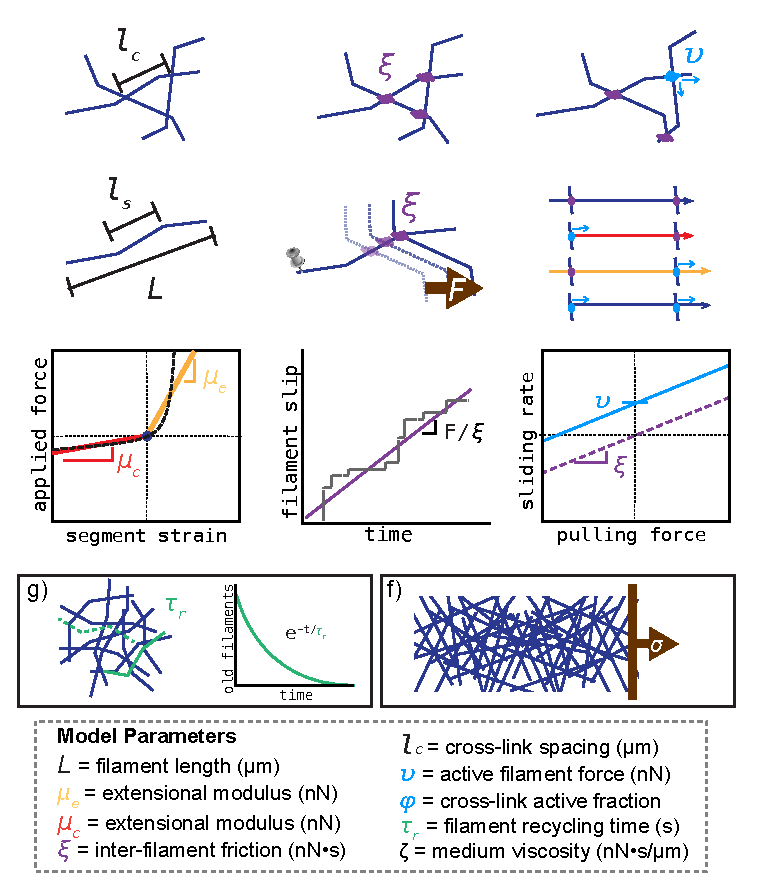
\includegraphics[width=\hsize]{figures/fig2/fig2}
\caption{\label{fig:sim} Schematic of modeling framework. a) Asymmetric filament compliance.  Filaments have smaller spring constant for compression than for extension. b) Cross-link slip.  Cross-links are coupled by an effective drag, such that their relative motion is proportional to any applied force. c) Motor activity. Filament activity manifests as a basal sliding rate even in the absence of an external force. d) Fractional activity.  Only a subset of filament cross-links are active, resulting in differential force exertion along the filament.  e)  Filament recycling.  Filaments are turned over at a constant rate, leading to a refreshing in the strain state of all filaments after a characteristic timescale.}
\end{figure}

We choose to focus our attention on 2D networks both for their tractability as well as their relevance in the quasi-2D cytoskeletal cortex of many eukaryotic cells\cite{cellmech_flows}.  In addition, recent developments in 2D {\em in vitro} systems\cite{rheo_2D1,rheo_2D2}, make 2D disordered models all the more interesting as a renewed focus of study.  In the rest of this section, we underline the key points necessary for understanding our modeling framework and the key assumptions we have made in generating our equations of motion for the system.


\subsection*{Asymmetric Filament Compliance}
We model individual filaments as chains of springs with relaxed length $l_s$.  Filaments can therefore be represented as a sequence of nodes with positions $\mathbf{x_i}$ and nearest neighbor force interactions, $\mathbf{F_i}$, of the form

\begin{equation}
|F_i| = \mu\cdot\frac{|\mathbf{x_{i+1}}-\mathbf{x_i}|-l_s}{l_s} +\mu\cdot\frac{|\mathbf{x_{i-1}}-\mathbf{x_i}|-l_s}{l_s}
\end{equation}





where, $\mu$ represents an extensional modulus of a filament.   Here, we take the modulus, $\mu$, to have a different value depending on whether $|\mathbf{x_{i-1}}-\mathbf{x_i}|-l_s$ is greater or less than 0.  This moduli is a composite quantity related to both filament and cross-linker compliance in a manner similar to a proposed effective medium theory\cite{theo_crosslinknonlinear}.  In the limit of highly rigid cross-links and flexible filaments, our model reduces to the pure semi-flexible filament models of \cite{theo_hlm,theo_hlm2}.  In the opposite regime of nearly rigid filaments and highly flexible cross links, our method is still largely similar to the model of \cite{theo_crosslinknonlinear} in small strain regimes before any nonlinear cross link stiffening.  However, in departure from those models, the magnitude of the force on interior cross-links in our model is still the same as those on the exterior.  This is a simplification of the varying levels of strain that would actually be present in these cross-linkers as addressed in \cite{theo_crosslinknonlinear}, but we choose to ignore the slight variation in favor of an approximated, global mean approach.  



\subsection*{Drag-like Coupling Between Overlapping Filaments}
\label{exp_drag}
Cross-link binding and unbinding is an important element of the overall stress relaxation of a network.  In contrast to previous models, we allow relaxation of the network's stored stress by letting the attachment points slip.  We do this by replacing an elastic interaction between pairs of points along filament segments with a drag-like coupling between segments.
\begin{equation}
\mathbf{F_{drag}} = \xi \cdot \int ds \: (\mathbf{v_i(s)}-\mathbf{v_j(s)}) \: p_{ij}(s)
\end{equation}

Where $p_{ij}(s)$ represents the locational distribution of cross-link points (equal to 1 at locations of cross-links and 0 elsewhere) and $\mathbf{v_i(s)}$ and $\mathbf{v_j(s)}$ represent the the velocities of the $i$th and $j$th filament segment.  This model assumes a linear relation between applied force and the velocity difference between attached segments.  This drag-like coupling has been shown to be an adequate approximation in the case of ionic cross-linking of actin\cite{mol_fric,theo_hydroish2}, and can be found in the theoretical basis of force-velocity curves for myosin bound filaments\cite{theo_frictionShila}. Although non-linearities can arise through force dependent detachment kinetics and/or non-linear force extension of cross-links, we assume that inhomogeneities from non-linear effects are of second or higher order. With this assumption, the motion for the entire network is governed by a dynamical equation of the form

\begin{equation}
\label{eqn:syst}
\int ds \: (\mathbf{\zeta v_i(s)} + \xi \sum _j(\mathbf{v_i(s)}-\mathbf{v_j(s)}) \: p_{ij}(s))= \mathbf{F_i}
\end{equation}

Here, the first term in the integral is the filament's intrinsic drag through its embedding fluid, $\zeta$, while the second comes from the drag-like coupling between filaments, $\xi$.  

\subsection*{Active Coupling for Motor Driven Filament Interactions}

To add motor activity we select a subset of cross-linked points and impart an additional force of magnitude $\upsilon$ directed in the orientations of the individual filaments, $\mathbf{u_i}$.  This leads to a modification of the equation of motion to

\begin{equation}
\label{eqn:syst}
\int ds \: (\mathbf{\zeta v_i(s)} + \xi \sum _j(\mathbf{v_i(s)}-\mathbf{v_j(s)}) \: p_{ij}(s))= \mathbf{F_i}+\mathbf{u_i}\cdot\upsilon\int ds \sum _j \: p_{ij}(s)q_{ij}(s)
\end{equation}

In this formulation, only at the subset of points where  $p_{ij}(s)=1$ and $q_{ij}(s)=1$ will there be a force imparted.  In our simulations we let $q_{ij}$ be selected randomly such that $\bar{q}=\phi$, where $\bar{q}$ indicates the mean of $q$.


\subsection*{2D Network Formation}

We follow a mikado model approach by initializing a minimal network of connected unstressed linear filaments in a rectangular 2D domain.  We generate 2D networks of these semi-flexible filaments by laying down straight lines of length, $L$, with random position and orientation. We then assume that some fixed fraction of overlapping filaments become cross-linked (defined in \ref{exp_drag}) at their point of overlap.

Although real cytoskeletal networks may form with non-negligible anisotropy,  we  focus on isotropically initialized networks for simplicity.  We define the density using the average distance between cross-links along a filament, $l_c$. A simple geometrical argument can then be used to derive the number of filaments filling a domain as a function of $L$ and $l_c$\cite{theo_hlm}.  Here, we use the approximation that the number of filaments needed to tile a rectangular domain of size $W \times H$  is $2WH/Ll_c$, and that the length density is therefore $1/l_c$. In the absence of cross-link slip, we expect the network to form a connected solid with a well defined elastic modulus\cite{theo_hlm,theo_hlm2}.  


\subsection*{System of Equations for Applied Stress}
We model our full network as a coupled system of differential equations satisfying \ref{eqn:syst}.  Although the general mechanical response of this system may be very complex, we focus our attention on low frequency deformations and the steady-state creep response of the system to an applied stress.  To do this we introduce a fixed stress, $\sigma$ along the midline of our domain.  This stress points in the direction, $\mathbf{\hat{x}}$, producing extensional stress.

Finally, we add a 0 velocity constraint at the far edges of our domain of interest.  We assume that our network is in the "dry," low Reynold's number limit, where inertial effects are so small that we can equate our total force to 0.  Therefore, we have a dynamical system of wormlike chain filaments satisfying

\begin{equation}
\int ds \: (\zeta\mathbf{v_i(s)} + \xi \sum _j(\mathbf{v_i(s)}-\mathbf{v_j(s)}) \: p_{ij}(s)) = \mathbf{F_i}+\mathbf{u_i}\cdot\upsilon\int ds \sum _j \: p_{ij}(s)q_{ij}(s) + \sigma\mathbf{\hat{u}(x_i)}
\end{equation}

subject to constraints such that $\mathbf{v_i(x)}$ is 0 with $x=0$.  This results in an implicit differential equation for filament segments which can be discretized and integrated in time to produce a solution for the motion of the system.


\subsection*{Filament Recycling as a model for rapid filament turnover}

To simplify the complex biochemical changes that can give rise to actin filament polymerization and depolymerization, we chose to use simple filament appearance and disappearance as a lowest order model of filament recycling.  In this sense the average lifetime of a filament between it's appearance and disappearance would be $\tau_r$.  In order to do this without causing an unnecessary bias in the results, at a regularized interval $\tau_s < 0.01\cdot\tau_r$, we selected $\tau_s/\tau_r$ filaments, reset their extension or compression to 0, and relocated them to a random position and orientation.  This has the effect of creating an approximately exponential decay in the number of old filaments over time.


\subsection*{Computational Simulation Method}

We tested our analytical conclusions on a computational model.  More technical details of the model can be found in the Appendix, but we summarize the main modeling points here.

We discretize the filaments such that the equations of motion becomes a coupled system of equations for the velocities of filament endpoints, $\mathbf{x}$.  The drag-like force between overlapping filaments results in a coupling of the velocities of endpoints.  

\begin{equation}
\mathbf{A \cdot \dot x} = \mathbf{f(x)}
\end{equation}

where $\mathbf{A }$ represents a coupling matrix between endpoints of filaments that overlap, and $\mathbf{f(x)}$ is the spring force between pairs of filament segment endpoints.  We can then numerically integrate this system of equations to find the time evolution of the positions of all filament endpoints.

We generate a network by laying down filaments with random position and orientation within a domain of size $D_x$ by $D_y$ with periodic boundaries in the y-dimension.  The external stress (shear or extensional/compressional) is applied to all filament endpoints falling within a fixed x-distance from the center of the domain.  Finally, filament endpoints falling within a fixed x-distance from the edges of the domain are constrained to be nonmoving.



The nominal units for length, force, and time are $\mu m$, nN, and s, respectively.  We explored parameter space around an estimate of biologically relevant parameter values, given in Table \ref{table:para}. 

\begin{table}[h]
\centering
\caption{Simulation Parameter Values}
\label{table:para}
\begin{tabular}{|c|c|c|c|c|}
\hline
{\bf parameter}             & {\bf symbol} & {\bf physiological estimate}          \\ \hline
extensional modulus         & $\mu_e$        & $10 nN $                                               \\
compressional modulus             & $\mu_c$     & $ 0.1 nN $                           \\
cross-link drag coefficient & $\xi$      & $unknown $              \\
medium drag coefficient     & $\zeta$        & $0.0005 \frac{nN s}{\mu m^2} $      \\
filament length             & L            & $5 \mu m$                                          \\
cross-link spacing          & $l_c$        & $0.5 \mu m$                                         \\
domain size                 & $D_x\times D_y$            & $20\times 50 \mu m$                                 \\ \hline
\end{tabular}
\end{table}



% Results and Discussion can be combined.
\section*{Results and Discussion}

\subsection*{Actin turnover and actomyosin contraction play crucial roles in preserving sustained cortical flows in C. elegans embryos}

This will be a section where we introduce the problem with a bit of flow data as well as some data illustrating the disruption of flow in jasplakinolide treatment.

Near the end make a mention of the idealized model consisting of a contracting and an expanding domain.  This will allow a segue to the next two sections.

\subsection*{Filament recycling prevents cortical tearing and modulates the viscous stress relaxation of filament networks under external stress}

We first probed the effect of filament recycling on the network's passive response by imposing an external force on our simulated network.   As shown in Figure \ref{fig:passive} part a), by applying a force at the boundary of a patch of network, we induced a net strain.  On short timescales the networked responded mostly elastically by approaching a fixed strain $\gamma_0$, similar to that predicted by \cite{theo_hlm}.  However, on times longer than $\tau_c$, we found that the network approached a steady linear strain rate, characterized by an effective viscosity, $\eta$.  We were able to develop a simple theoretical description that captured the observed dependence.

\begin{equation}
\label{eqn:eff_vic}
\eta_c = \xi\left (\frac{L}{l_c}\right )^2
\end{equation}

It is interesting to note that as shown in Figure \ref{fig:passive}, the crossover time, $\tau_c$ is well described by the ratio of the effective viscosity, $\eta_c$, to the elastic modulus, $G_0 = \mu/l_c$.



\begin{figure}[h!]
\centering
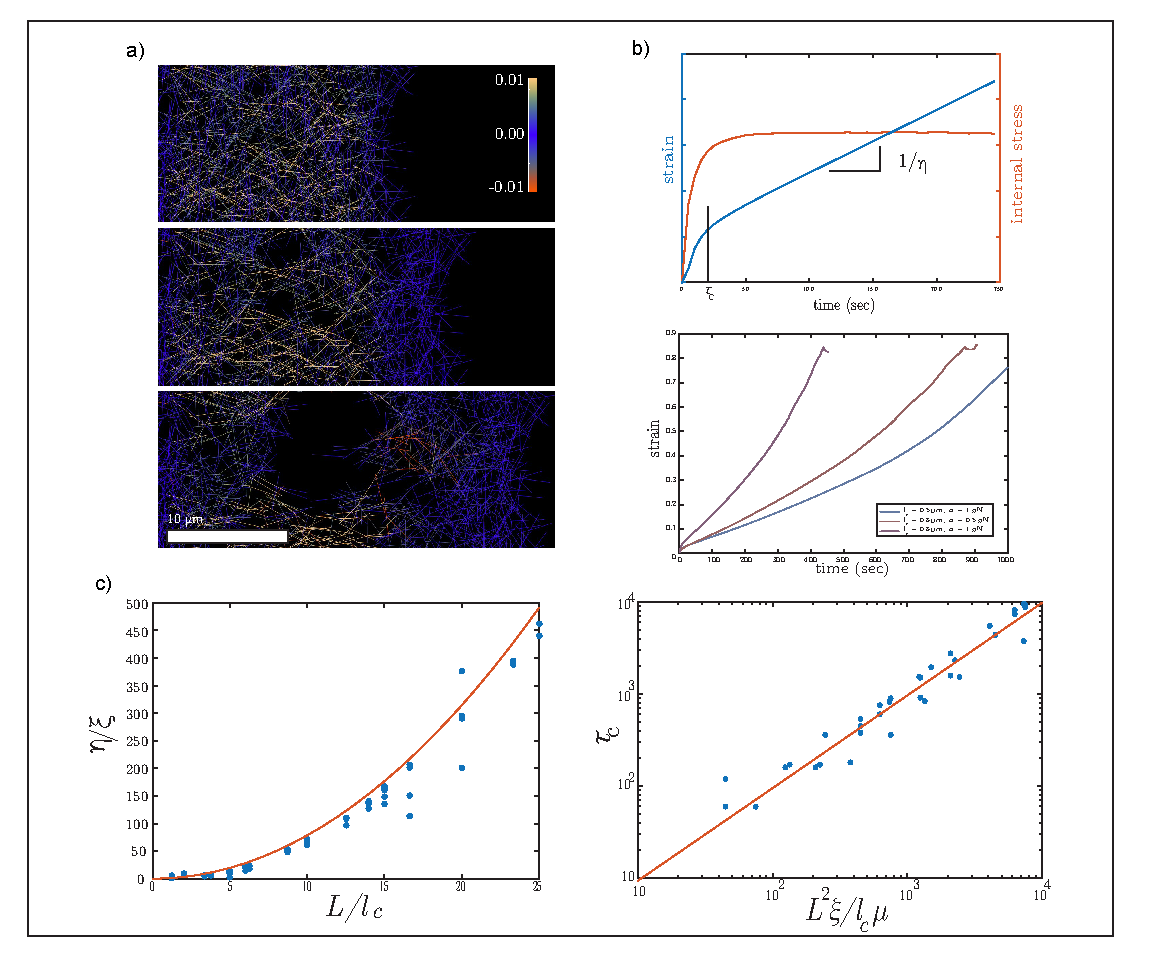
\includegraphics[width=\hsize]{figures/fig3/fig3}
\caption{\label{fig:passive} Filament recycling prevents cortical tearing and modulates the viscous stress relaxation of filament networks under external stress \textbf{a)} Network extension in the presence of cross-link slip alone. i. Example simulations of a network under and external applied extensional stress. ii. Example trace of the stress and strain buildup in an extending network.  The network begins to behave purely viscously at $\tau_c$, and the network deforms like a material with effective viscosity $\eta_c$. iii. The effective viscosity depends on the cross-link drag coefficient and the density of the network. iv. The timescale of the transition to viscous behavior has a characteristic dependence. \textbf{b)} Networks thin and tear at high strains. i. Example simulations of networks under extension at higher strains. ii. Example traces of networks in i.  iii.  Effective viscosity drops as networks are strained. \textbf{c)} Filament recycling rescues network tearing and modulates effective viscosity. i. Examples of same network under extension with and without recycling. ii.  Illustration of the difference in strain for identical network setups in the presence of different filament recycling rates. iii. Master curve for the dependence of filament strain rate on the timescale of filament recycling relative to timescale of cross link slip. }
\end{figure}



\subsection*{Filament recycling allows persistent stress buildup in active networks}

Next we tackled the case of a network with spatially isotropic motor activity.  We found that our simulation axioms were able to produce transient contraction of a patch of free-floating network.  As shown in Figure \ref{fig:active} a, the contraction extent was strongly dependent on the magnitudes of both the filament asymmetry and the motor activity scale.  Additionally, contraction would only occur when there was fractional motor activity, $\phi<1$, (see supplement).  The contraction was able to take place over a time scale, $\tau_c$, but on time scales much longer the contraction would stall and polarity sorting would begin to dominate.

Due to the long term polarity sorting and the fact that filament recycling would be difficult to incorporate into a moving material, we additionally analyzed the stress buildup in a patch that was constrained to maintain its original area.  As shown in Figure \ref{fig:active} b, the results showed a period of net stress due to an imbalance between larger stresses from extended filaments and smaller stresses from compressed filaments.  After a characteristic timescale $\tau_a$, the extensional stress peaks and begins to decrease while the compressive stresses continue to build up resulting in the extensional and compressive stresses beginning to cancel each other.  After another time period, $\tau_{eq}$, the internal stresses become balanced and the net stress drops to approximately 0. The timescale and magnitude of the peak stresses agree with a qualitative expectation discussed later.

Upon the addition of filament recycling, we were able to find that the network maintained a nonzero net stress for times much longer than $\tau_eq$.  We refer to this as the steady state stress because based on our simulations it doesn't appear that this stress ever subsides, and duh.  For similar network parameters as illustrated in Figure \ref{fig:active} c iii, we found that the steady state stress was well predicted by the comparison between the timescale of recycling, $\tau_r$ and that of peak activity, $\tau_a$. 


\begin{figure}[h!]
\centering
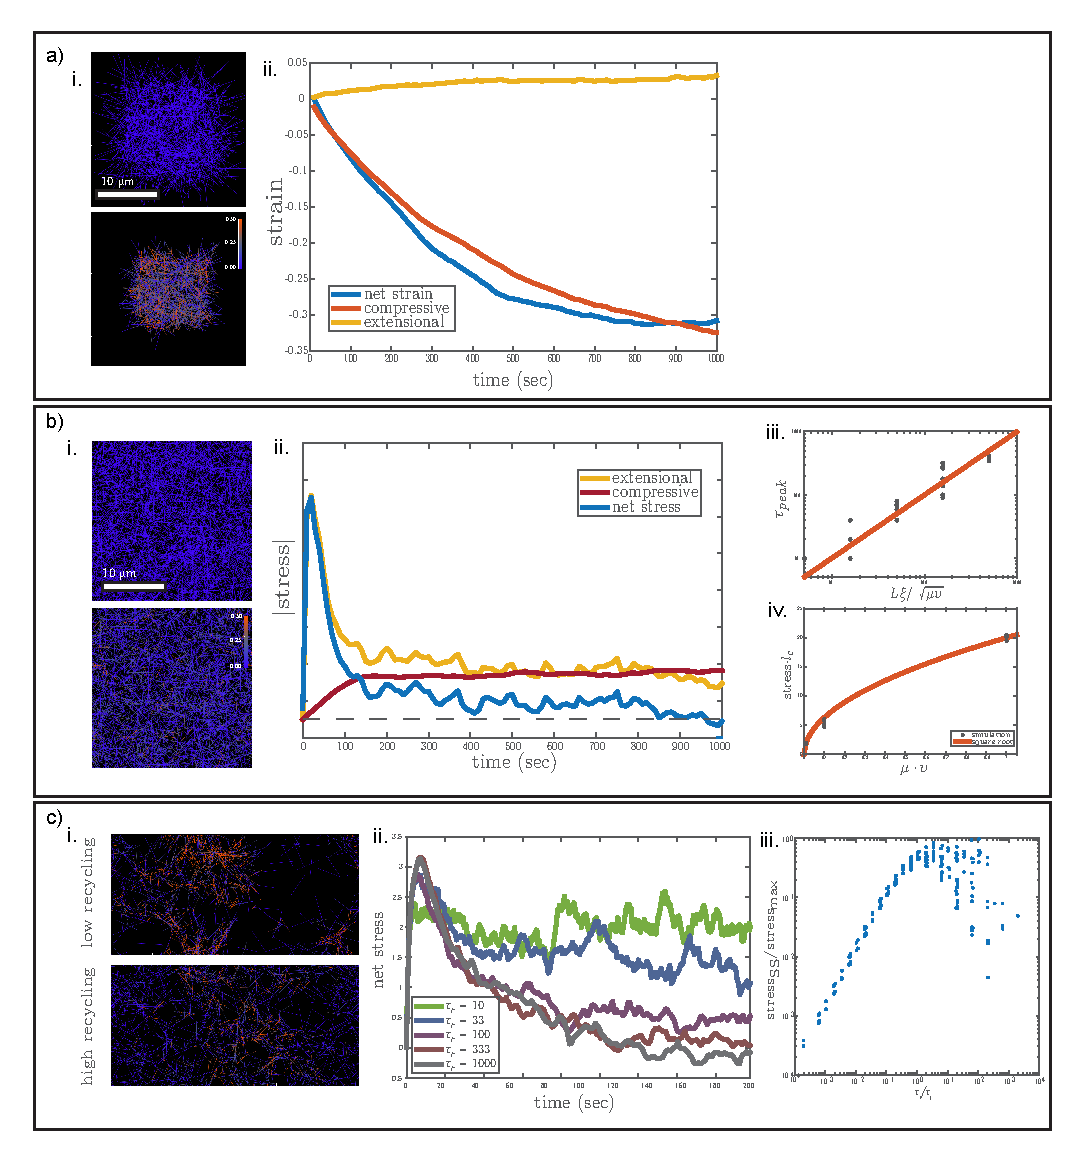
\includegraphics[width=\hsize]{figures/fig4/fig4}
\caption{\label{fig:active} Filament recycling allows persistent active stress buildup in active networks.  \textbf{a)} Network contraction. i. Example of an active network contracting. ii. Traces of total network strain and internal strain of filaments. \textbf{b)} Internal stress buildup is only transient. i. Example simulation of an active network building up internal stress while maintaining a constant area. ii. Traces of stress buildup. iii. Timescale of stress buildup. iv. Peak stress depends on myosin activity and filament stiffness. \textbf{c)} Filament recycling allows for steady state stress buildup. i. Example simulations of networks with fast and slow rates of recycling. ii. Traces of net stress for with different recycling timescales; faster recycling prevents the dress from relaxing entirely.  iii. Steady state stress depends on the recycling time relative to the crossly relaxation time. }
\end{figure}

\subsection*{Filament recycling modulates the balance between active stress buildup and viscous stress relaxation to set the flow rate in polarized networks}











\section*{Supporting Information}

% Include only the SI item label in the subsection heading. Use the \nameref{label} command to cite SI items in the text.

\section*{Acknowledgments}
We would like to thank Shiladitya Banerjee and Patrick McCall for stimulating discussions.

\nolinenumbers

%\section*{References}
% Either type in your references using
% \begin{thebibliography}{}
% \bibitem{}
% Text
% \end{thebibliography}
%
% OR
%
% Compile your BiBTeX database using our plos2015.bst
% style file and paste the contents of your .bbl file
% here.
% 
\bibliographystyle{plos2015}
\bibliography{slippage,active}

\begin{comment}
\begin{thebibliography}{10}
\bibitem{bib1}
Devaraju P, Gulati R, Antony PT, Mithun CB, Negi VS. Susceptibility to SLE in South Indian Tamils may be influenced by genetic selection pressure on TLR2 and TLR9 genes. Mol Immunol. 2014 Nov 22. pii: S0161-5890(14)00313-7. doi: 10.1016/j.molimm.2014.11.005

\bibitem{bib2}
Huynen MMTE, Martens P, Hilderlink HBM. The health impacts of globalisation: a conceptual framework. Global Health. 2005;1: 14. Available: http://www.globalizationandhealth.com/content/1/1/14.

\end{thebibliography}
\end{comment}


\end{document}


% Template for PLoS
% Version 3.1 February 2015
%
% To compile to pdf, run:
% latex plos.template
% bibtex plos.template
% latex plos.template
% latex plos.template
% dvipdf plos.template
%
% % % % % % % % % % % % % % % % % % % % % %
%
% -- IMPORTANT NOTE
%
% This template contains comments intended 
% to minimize problems and delays during our production 
% process. Please follow the template instructions
% whenever possible.
%
% % % % % % % % % % % % % % % % % % % % % % % 
%
% Once your paper is accepted for publication, 
% PLEASE REMOVE ALL TRACKED CHANGES in this file and leave only
% the final text of your manuscript.
%
% There are no restrictions on package use within the LaTeX files except that 
% no packages listed in the template may be deleted.
%
% Please do not include colors or graphics in the text.
%
% Please do not create a heading level below \subsection. For 3rd level headings, use \paragraph{}.
%
% % % % % % % % % % % % % % % % % % % % % % %
%
% -- FIGURES AND TABLES
%
% Please include tables/figure captions directly after the paragraph where they are first cited in the text.
%
% DO NOT INCLUDE GRAPHICS IN YOUR MANUSCRIPT
% - Figures should be uploaded separately from your manuscript file. 
% - Figures generated using LaTeX should be extracted and removed from the PDF before submission. 
% - Figures containing multiple panels/subfigures must be combined into one image file before submission.
% For figure citations, please use "Fig." instead of "Figure".
% See http://www.plosone.org/static/figureGuidelines for PLOS figure guidelines.
%
% Tables should be cell-based and may not contain:
% - tabs/spacing/line breaks within cells to alter layout or alignment
% - vertically-merged cells (no tabular environments within tabular environments, do not use \multirow)
% - colors, shading, or graphic objects
% See http://www.plosone.org/static/figureGuidelines#tables for table guidelines.
%
% For tables that exceed the width of the text column, use the adjustwidth environment as illustrated in the example table in text below.
%
% % % % % % % % % % % % % % % % % % % % % % % %
%
% -- EQUATIONS, MATH SYMBOLS, SUBSCRIPTS, AND SUPERSCRIPTS
%
% IMPORTANT
% Below are a few tips to help format your equations and other special characters according to our specifications. For more tips to help reduce the possibility of formatting errors during conversion, please see our LaTeX guidelines at http://www.plosone.org/static/latexGuidelines
%
% Please be sure to include all portions of an equation in the math environment.
%
% Do not include text that is not math in the math environment. For example, CO2 will be CO\textsubscript{2}.
%
% Please add line breaks to long display equations when possible in order to fit size of the column. 
%
% For inline equations, please do not include punctuation (commas, etc) within the math environment unless this is part of the equation.
%
% % % % % % % % % % % % % % % % % % % % % % % % 
%
% Please contact latex@plos.org with any questions.
%
% % % % % % % % % % % % % % % % % % % % % % % %

\documentclass[10pt,letterpaper]{article}
\usepackage[top=0.85in,left=2.75in,footskip=0.75in]{geometry}

% Use adjustwidth environment to exceed column width (see example table in text)
\usepackage{changepage}

% Use Unicode characters when possible
\usepackage[utf8]{inputenc}

% textcomp package and marvosym package for additional characters
\usepackage{textcomp,marvosym}

% fixltx2e package for \textsubscript
\usepackage{fixltx2e}

% amsmath and amssymb packages, useful for mathematical formulas and symbols
\usepackage{amsmath,amssymb}

% cite package, to clean up citations in the main text. Do not remove.
\usepackage{cite}

% Use nameref to cite supporting information files (see Supporting Information section for more info)
\usepackage{nameref,hyperref}

% line numbers
\usepackage[right]{lineno}

% ligatures disabled
\usepackage{microtype}
\DisableLigatures[f]{encoding = *, family = * }

% rotating package for sideways tables
\usepackage{rotating}

\usepackage{verbatim}   % useful for program listings

% Remove comment for double spacing
%\usepackage{setspace} 
%\doublespacing

% Text layout
\raggedright
\setlength{\parindent}{0.5cm}
\textwidth 5.25in 
\textheight 8.75in

% Bold the 'Figure #' in the caption and separate it from the title/caption with a period
% Captions will be left justified
\usepackage[aboveskip=1pt,labelfont=bf,labelsep=period,justification=raggedright,singlelinecheck=off]{caption}

% Use the PLoS provided BiBTeX style
% \bibliographystyle{plos2015}
\bibliographystyle{apalike}

% Remove brackets from numbering in List of References
\makeatletter
\renewcommand{\@biblabel}[1]{\quad#1.}
\makeatother

% Leave date blank
\date{}

% Header and Footer with logo
\usepackage{lastpage,fancyhdr,graphicx}
\usepackage{epstopdf}
\pagestyle{myheadings}
\pagestyle{fancy}
\fancyhf{}
\lhead{\includegraphics[width=2.0in]{PLOS-submission.eps}}
\rfoot{\thepage/\pageref{LastPage}}
\renewcommand{\footrule}{\hrule height 2pt \vspace{2mm}}
\fancyheadoffset[L]{2.25in}
\fancyfootoffset[L]{2.25in}
\lfoot{\sf PLOS}

%% Include all macros below

\newcommand{\lorem}{{\bf LOREM}}
\newcommand{\ipsum}{{\bf IPSUM}}

%% END MACROS SECTION


\begin{document}
\begin{figure}[h!]
\centering
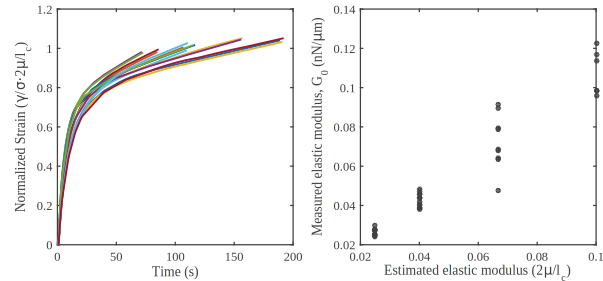
\includegraphics[width=\hsize]{figures/figure3S}
\caption{\label{fig:passive_rec}  Filament recycling rescues network tearing and modulates effective viscosity.  \textbf{a)} Examples of $20 \times 12 \mu m$ network under 0.001 $nN/\mu m$ extensional stress with recycling ($\tau_r=10 s$) and without, ($\tau_r=\infty$).  Both images are taken when the patches had reached a net strain of 0.4.  The network with recycling doesn't appear to change shape because its components have been recycled to remain in the original domain.  Network parameters: $L=3\: \mu m$, $l_c=0.5\: \mu m$, $\xi=10\: nN\cdot s$.  \textbf{b)}  Strain buildup for networks with parameters as in a) in the presence of different filament recycling rates. Dotted line indicates the strain state at which the snapshots in panel a) were taken.  Note that the strain rate for $\tau_r=1000$ is essentially identical to that of $\tau_r=\infty$, indicating that recycling does not govern the relaxation rate if the recycling time is above a threshold.}
\end{figure}

\begin{figure}[h!]
\centering
\includegraphics[width=\hsize]{figures/figure6S}
\caption{\label{fig:passive_rec}  Filament recycling rescues network tearing and modulates effective viscosity.  \textbf{a)} Examples of $20 \times 12 \mu m$ network under 0.001 $nN/\mu m$ extensional stress with recycling ($\tau_r=10 s$) and without, ($\tau_r=\infty$).  Both images are taken when the patches had reached a net strain of 0.4.  The network with recycling doesn't appear to change shape because its components have been recycled to remain in the original domain.  Network parameters: $L=3\: \mu m$, $l_c=0.5\: \mu m$, $\xi=10\: nN\cdot s$.  \textbf{b)}  Strain buildup for networks with parameters as in a) in the presence of different filament recycling rates. Dotted line indicates the strain state at which the snapshots in panel a) were taken.  Note that the strain rate for $\tau_r=1000$ is essentially identical to that of $\tau_r=\infty$, indicating that recycling does not govern the relaxation rate if the recycling time is above a threshold.}
\end{figure}
\end{document}



\chapter{A model of upstream actomyosin regulators in pulsed contractions}
\input{pulse/pulse_paper}

\chapter{Conclusions, Open Issues, \& Future Directions}

\section{Conclusion}
In this work I have presented my attempts to measure and model the dynamics of cortical flow. I have done this by assisting in developing a technique to improve our ability to measure actin dynamics in the cell cortex, and by developing mechanistic models of actomyosin and its upstream regulators. Although this work was able to establish several useful findings, there were shortcomings in the methodology used and the assumptions implicit in the modeling framework.  In the next section, I outline shortcomings in my modeling methodology and potential ways to resolve those shortcomings in the near term. I discuss some of the limitations and broader implications of the model presented in Chapter 3. Next, there have been some very recent publications that have undertaken to explore the same subject area that I have described in this thesis, namely actomyosin dynamics with turnover.  In Section \ref{sec:compar_lit}, I compare my work to two of the most pertinent studies, and draw conclusions about the generality or specificity of findings in each work.  Finally, I end this chapter with a description of a simple set of experiments that I believe will be beneficial in validating the theoretical conclusions of my modeling efforts.



\section{Limitations of the present modeling approach and how these could be addressed in future work}

\subsection{Pure friction for cross-link interaction}
A key feature of my model in comparison to others is that the mechanism of cross-linking is a frictional coupling between filaments.  The motivation for this (as discussed above) is to provide a mechanism of coupling filaments on short timescales while allowing the rearrangement of filaments on long-timescales.  Frictional coupling serves as a simplification of the processes of cross-linking binding, deformation under force, and unbinding, and has been used previously \cite{theo_friction,theo_frictionSam,theo_molefric,mol_fric,theo_hydroish2,theo_frictionShila} to effectively simplify the aggregated action of many molecular binding and unbinding events. In Appendix \ref{chap:slippage}, I give a detailed account of how one could derive such a frictional coupling from the averaging of many reversible elastic attachments.  

Nevertheless, the assumptions used in generating this frictional coupling are a generalization and it is possible that specific details governing the cross-linking in cells could impact the physics in ways that my model cannot account for.   For example, my particular implementation of frictional coupling necessitates that the coupling is linear in the velocity, but theoretically any force-velocity relationship could exist between the two cross-linked filaments.  By modifying the equations of motion, I could theoretically incorporate non-linearities in the force-velocity curve, allowing, for example, a frictional coupling that was dependent on the square or the cube of the velocities.  However, it seems that this would only have an impact on the quantitative relationships between, say, applied stress and network strain rate, giving rise to non-Newtonian viscosities.  While this would make the analysis much more complicated due to the inability to scale out things like applied stress, it wouldn't have much of an impact on the qualitative shape of the results I've drawn.

A more serious concern is the possibility that even on very long timescales, the filaments do not experience purely viscous coupling at all, but that some amount of elastic constraint exists indefinitely.  This could arise from effectively irreversible cross-link binding, or from another active process which serves to prevent filament rearrangement after they reach a stable deformed configuration (e.g. alignment of bundles could stabilize particular deformed geometries).  The present implementation of my model does not allow for any irreversible attachments of cross-linkers.  However, in a certain sense, my model is able to mimic irreversible cross-linking by allowing the frictional coupling to be arbitrarily high.  It might be interesting to explore how networks respond to a subset of filaments undergoing cross-link rearrangement on disparate timescales in future work. This might have several interesting effects.  It would probably affect the timescale of transition to viscous flow in passive networks and impede local rearrangements that lead to dissipation of contractile stress on short timescales.  These two effects would complicate the dependence of steady state stress and effective viscosity on network parameters on longer timescales, impacting the conclusions I've drawn about the rates of flow.  


\subsection{Linearization of filament compliance and myosin force-velocity}
Another simplification assumed in my model is the piecewise linearization of the filament force extension curve and the myosin force-velocity curve. In both cases my model can easily be extended to incorporate more subtle details of the relationship, similar to the case for linear friction, but I believe that this extension will only make the model increasingly complex without changing the qualitative outcomes, as I will explain below.

First, the linear approximation of the myosin force-velocity curve is unlikely to alter the main predictions of the model for the same reason as linearization of the cross-link friction force-velocity curve.  The actual relationship between stall force and velocity resembles an inverse relationship rather than a negatively sloping linear relationship as I approximate it in the model \cite{howard2001mechanics}.  Thus, as the real  motor transitions from freely moving to stalled it will not transition linearly, but will initially build force slowly and then more rapidly as it reaches stall.  This will have some very subtle impacts on the time progression of force buildup, but it is unlikely that there would be any major effects that could prevent force buildup or stall altogether.  Thus the time series of force buildup could be different, but the qualitative effect would be the same.

The piecewise linearization of the force extension curve as a worm-like chain is a bit more complicated.  The simple linearization makes it incredibly simple to model a general semi-flexible filament-like structure, which can include an actin, a microtubule, a bundle of actin filaments, or a carbon nanotube, in a manner that is agnostic to the specific non-linear relationship that arises due to the local mechanics and geometry.  However, in order to generalize the asymmetry between contraction and extension, one still has to select a threshold to define the two windows of strain.  In my model, I used an arbitrary distinction between extension and compression around the relaxed length, but this is an oversimplification.  In reality, the non-linearity could arise at some offset extension (if one were  interested in slack being pulled out of the filament) or compression (if one were interested in buckling).  Needless to say, this offset could easily be added to the piecewise linearization process without complicating the analysis much further.  Additionally, this linearization is very useful to gain analytcal insight as it allows the asymmetry factor to fall out of the any measurements regardless of the specific deformation regime that is being probed in a given simulation.  In contrast, if one were to look at a wormlike chain model instead, they would find that for some deformations there would be no asymmetry, then for slightly more deformation there would be a factor of, say, 10 asymmetry and then for even more deformation you would reach an infinite difference between extension and contraction.  Thus, you must draw all of your conclusions relative to the specific window of deformation, and some of the general structure of the mechanical picture can be lost.  In contrast, the linearization means that for any deformation the difference in the force applied between extension and compression will be a constant.  While this is advantageous for making the analysis very clear, it has the drawback of making the network's rigidity linear when it would actually show many more interesting non-linear properties.  However, if one were interested in making quantitative predictions for a very particular and well-characterized kind of filament network, a more detailed force-extension curve could easily be implemented in this framework.

\subsection{Absence of Thermal fluctuations}
In my model, I do not incorporate any thermal fluctuations into the motion of filaments or motors.  For individual filaments in solution, thermal fluctuations can give rise to large filament deformations and long-range diffusion \cite{PhysRevE.69.061921}.  However, it is unclear how important these motions are on the timescales of interest when cross-linking connects the network into a macroscopic structure.  Single molecule measurements  in \textit{C. Elegans} embryos \cite{Robin:2014aa} suggest actin filaments are subdiffusive ($\langle r^2 \rangle = Dt^{0.6}$) with very low short term diffusivity ($D = 0.057 \mu m^2 /s$).  In contrast, the advective flows found in embryos and motile cells move material at upwards of ten microns per minute \cite{Munro2004413, amoeba1, amoeba3}.  This results in a Peclet number between 3 and 6, and allows us to assume that for flowing cortices, advective motion of the connected network dominates.

Because the goal of this work is to derive general properties of how flows of any speed arise, I also want to point out that this non-thermal description can be coupled with an understanding that diffusive motion can sometimes dominate.  Since we can always demark a difference in flow speeds between those networks where the macroscopic motion dominates versus those where diffusive effects dominate, one can ignore thermal effects provided we remember that at low enough advection speeds diffusion will again dominate. I assume that any time I observe very little motion in my simulations, a real system will be in an effectively diffusive state and we can use our understanding of passive networks to describe the thermal motions of the filaments.  Thus, when my simulations result in very small flow rates, I assume that these flows will fail to outpace diffusion and, therefore, will be effectively nullified.  However, in the future, it may be worthwhile to explicitly incorporate these effects in order to directly observe the transition between diffusive and advective motion.

\section{Probing more complex mechanisms of turnover}

Another notable simplification in this work is the method of incorporating filament turnover. The mechanism I employed causes entire filaments to be reset at random, which may not accurately reflect  the mechanisms by which filaments are depolymerized and repolymerized in living cells. Filament depolymerization and repolymerization are governed by more complex processes that have been studied in painstaking detail \textit{in vitro}, but which have not been well-characterized in cells \cite{doi:10.1146/annurev-biophys-051309-103849, Robin:2014aa}.  From \textit{in vitro} experiments we know that filaments can turn over through treadmilling \cite{doi:10.1146/annurev-biophys-051309-103849}, severing \cite{bemenet}, or a more complex process call actin bursting \cite{Kueh2008}.  The net result of these events will cause rapid and complete strain resetting on long enough timescales, but differences in mechanisms of turnover could  change the exact form of the strain and orientation resetting of filaments.

The mechanisms for filament depolymerization rely on a balance of slow filament treadmilling, accompanied by faster filament severing events.  The combined action of these two mechanisms should cause a rapid removal of the filament from the physically connected network and thus cause an effectively immediate stress dissipation much like the one demonstrated in our model. Nevertheless, there may be many regulatory factors which act to make the stress dissipation less idealized than in the simplified model.  One such complicating factor would be stress dependent severing rates \cite{Hayakawa721, Murrell:2015aa}, which would cause non-uniform dissipation of stress or preservation of stress, depending on whether filaments were preferentially severed based on being in a high stress or low stress state, respectively. It will be interesting in the future to explore how different modes of disassembly might contribute differently to shaping contractile dynamics and cortical flow.

In addition to non-uniform depolymerization, there are also molecular details that impact our assumptions about repolymerization. In my model, freshly polymerized filaments are assumed to appear with a random orientation, and all filaments are assumed to be polymerized to a uniform length.  Both of these simplifying assumptions may be violated in real systems. For example, recent work in our group (Younan Li, unpublished) suggests that there may be biases in the orientation of newly polymerized filaments.  Specifically, formins appear to follow existing actin filaments preferentially, thereby laying down a new actin filament along a template of an existing filament (Younan Li, unpublished).  In addition, crosslinking proteins can preferentially align (or in some cases obstruct the alignment of) newly polymerized actin \cite{Falzone2012}.  This may be an important part of regulating stress asymmetries and as such may need to be incorporated into some aspects of active network models in the future.  

The end result of these complex processes allows stress resetting to occur independently from orientational resetting.  In this sense, the simplifications in the current implementation tend to conflate the processes of stress resetting and orientation resetting. In effect, there may be different timescales over which different aspects of network memory relax.  Understanding how this works is  an important avenue of future work.


\subsection{Which is more important, local density equilibration or stress resetting?}
It seems very clear that  global disruption of connectivity will necessarily lead to an inability to maintain global net stresses.  However, in this work, I've argued that one need not develop global loss of connectivity in order for the net stress to dissipate. I found that even if networks remain macroscopically connected,  local rearrangements within the network have a tendency to decrease extensional and increase compressional stress, leading to a dissipation in net global contractile stress across the network.   Therefore, there are actually two distinct activities that occur when filaments are recycled in my model: 1) new filaments appear where there may be fewer filaments, resulting in local density equilibration, and 2) they are reset to have no strain.  

This begs the question: Which is more important, local density equilibration or stress resetting?

My results suggest that it is stress resetting which is ultimately more important than density equilibration.  Overall, if the thinning from global rearrangement was apparent, then one would have to equilibrate density to maintain connectivity.  However, without resetting strain, the filaments would still be able to reach internal balance between extension and compression.  In other scenarios, where there is no global thinning, the net stress is still lost over time due to the local rearrangements and extensional and compressive balancing. It would be easy to test this with the framework I have put in place.  One could decouple the two mechanisms by redistributing filaments as they turnover without changing their strain state, and  reset their strain without moving them to new areas.  If I were to equilibrate the network density by relocating filaments to regions where connectivity was being lost, but I was to retain them in their stressed state, I predict that the net stress would still be lost.  

\subsection{Overlooking the subtleties of myosin turnover}
Another possible contribution to maintaining steady state stress would be the turnover of Myosin II minifilaments.  My model lacks any direct mechanism by which motor turnover can be implemented---i.e. The subset of filament crossovers at which myosin II is active is fixed throughout the simulation. A more realistic model would allow dynamic transitions in motor activity at crossover points.  This would mean that over time the dynamic imbalance of compressive vs extensional stress on individual filaments could be reset, even without local rearrangement.

Indeed, it is possible that filament turnover is not actually required to allow stresses to persist.  Instead, it may be possible that a steady state level of net stress could be maintained indefinitely by the constant deactivation and reactivation of motor activity.  In principle, this could give rise to a form of stress resetting similar to the mechanism found with filament recycling.  As such, filament recycling could end up being redundant.  Nevertheless, it's possible that myosin turnover would not be capable of completely resetting filament stress because the filament stress relaxation would not be instantaneous as it is with filament recycling.

It would be easy to address this concern by modifying the simulation framework.  A simple implementation would allow random switching of motor activity on and off with yet another characteristic timescale, say $\tau_\tau$.  In this case, it would seem reasonable that the stress state of the network would be dependent on the minimum of the filament recycling timescale mentioned above ($\tau_r$) and the myosin turnover timescale ($\tau_\tau$).

\section{Comparison with Recent Modeling Publications}
\label{sec:compar_lit}
Several recent studies have incorporated turnover in computational models of actomyosin networks, and considered how filament turnover affects  timescales of stress generation and dissipation.  In the following two sections, I will compare my work with the results found in the two most pertinent recent papers.

\subsection{Role of Turnover in Active Stress Generation in a Filament Network by Tetsuya Hiraiwa and Guillaume Salbreux}
Hiraiwa and Salbreux \cite{2015arXiv150706182H} considered networks of actin filaments and  active motors and passive crosslinkers. Like us, they found that such networks are capable of generating only transient stresses, but adding filament turnover allows those stresses to be maintained indefinitely. They also showed that there is a critical number of cross-linkers required in order for the network to generate stress.  Below, I examine  their model in detail and compare it to my own. 

Hiraiwa and Salbreaux's model consisted of rigid filaments and rigid motors in the presence of passive cross-linkers.  They assumed that passive cross-linkers are point-like and bind rigid filaments together directly at their point of contact.  From this it follows that the cross-linking constraint only allows deformation through filaments rotating around their points of contact.  In addition, it should be clear that in this scenario three filaments attached in a triangle will not be able to undergo any deformation.  In their model, active force generation occurs when a motor walks along two actin filaments that are cross-linked together at one point.  The motor exerts a force on the two filaments which can serve to either contract or extend the filaments relative to each other.  Averaging over the total number of configurations before the motor detaches, they find, using a geometrical argument, that a single motor acting on  two actin filaments has a net bias toward contraction.  In this model, the contractile asymmetry arises from a finite size myosin.  By imposing that myosin has a finite size (along with imposing rigid cross-linking), the researchers generate an asymmetry between the ability of a myosin to walk toward a cross-linker vs away from a cross-linker.  Walking toward a cross-linker, the myosin acts to make the two filaments more perpendicular (driving endpoints apart and generating extensional force), while walking away from the cross-linker makes them more parallel (driving filament endpoints together and generating contraction). When averaging over the forces required to generate inward vs outward motion in this geometrical scenario, it can be determined that contraction is more favorable than extension \cite{PhysRevX.4.041002}. In my simulations, this effect would not take place at all, because myosins were assumed to act only at the intersection of filaments, and as such, the source of contraction is not due to  finite size myosin asymmetry, but instead to the asymmetric compliance of actin filaments.  Indeed, the geometrical argument underlying their source of contraction requires myosin motors to be fairly large relative to the actin filaments in order for this effect to be significant, as was shown in \cite{PhysRevX.4.041002}.  Based on the arguments on the physiological relevance of different mechanisms of contraction given in \cite{PhysRevX.4.041002} (see Lenz's phase diagram in Figure 5 of  \cite{PhysRevX.4.041002}), it would seem that the finite size myosin effect will be the governing behavior only in a small region of parameter space, and therefore it is perhaps not the most pertinent mechanism for focus.

Second, Hiraiwa and Salbreaux's model predicted that a critical number of cross-linkers are required for net stress to be generated within the network.  Interestingly, this critical number turns out to be equal to the number of filaments present in the network.  This makes intuitive sense, because if there were fewer cross-linkers than filaments, then there would be, on average, less than one cross-linker per filament. Thus most filaments would only be attached to one other filament, and the network would be unable to transmit forces over longer distances.  In my model, cross-linking was assumed to take place at every filament overlap point, and thus, by construction, my model always surpassed the critical cross-linking concentration, so long as the number of overlaps per filament is significantly greater than one. Indeed, Head and colleagues \cite{theo_hlm} have previously shown that for a geometry of randomly oriented filaments in 2D, the average number of overlaps per filament needs to be approximately 6.8 in order to reach macroscopic percolation.  If I relaxed the requirement that all overlap points represent a cross-link in my model, thus reducing the number of cross-linking points, I predict it would result in a similar effect to what was found in Hiraiwa and Salbreaux's study.  

Third, Hiraiwa and Salbreaux's networks can generate and maintain macroscopic stress, but allowing  cross-linker turnover prevented stresses from persisting.  If cross-links were allowed to turn over, filaments and motors were able to freely rearrange.  This free rearrangement led to loss of connectivity, clumping of filaments and motors, and dissipation of stress. This conclusion has been observed previously in \cite{Alvarado:2013aa} where they found that motors drive networks towards a critically connected state.  My model predicts a similar outcome, in which viscous cross-link slippage results in a global loss of network connectivity and macroscopic stress.  In my work, however, this was incorporated into cross-linking from the beginning, so all that could be varied was the timescale over which stress dissipation took place.  However, when I make my interfilament friction coefficient very high, I observe only an elastic response on short timescales.  Thus, their results for irreversible cross-linking are essentially equivalent to the limiting case of my model where the friction coefficient goes to infinity.


One of Hiraiwa and Salbreaux's key observations is that filament turnover allows their model network to maintain non-zero stress indefinitely, even with cross-link turn over.  Their explanation of this effect is similar to the explanation that I give in Chapter \ref{sec:core} (see page \pageref{pg:explainit}). When active motors rearrange filaments they cause a loss of connectivity, but this can be prevented by inserting new filaments into rarefied regions of the network. They show examples of this behavior to support their argument and interestingly, these cases also demonstrate that the critical number of cross-linkers they identified qualitatively holds for the case of turnover.  In contrast to their work, I also see a second mode of stress dissipation, which they do not mention in their work.  I will address the absence of this second mode in both Hiraiwa's work and in the work of Mak et al.  in a later section. 

Finally, Hiraiwa and Salbreaux present a phase diagram that summarizes their main conclusions. They showed that there was an optimum turnover time and that the optimum varied with the number of cross-linkers.  The more cross-linkers the network contained, the faster the turnover had to occur in order to reach the optimum.  Because the number of cross-linkers was not varied in my simulations, I could not draw any similar conclusions on this topic.

Hiraiwa and Salbreaux did not examine passive dissipation of stress in the absence of active stress generation, as I have done. However, based on their analysis of active stress, I predict that if they were to probe the passive response of their model networks (i.e. in the absence of active crosslinks) to applied stress, their model networks would not  maintain global connectivity if the number of cross-linkers was less than the number of filaments or in the presence of cross-link turnover the network. This is because, as I discussed above, having fewer than one cross-link per filament will likely lead to a global loss of connectivity over a large spatial scale.   

\subsection{Interplay of active processes modulates tension and drives phase transition in self-renewing, motor-driven cytoskeletal networks by    Michael Mak, Muhammad H. Zaman, Roger D. Kamm \& Taeyoon Kim}

The model of Mak et al. \cite{Mak:2016aa} is one of the most detailed models used to simulate actomyosin mechanics in the field.  As such, it is very useful for suggesting the origins of emergent properties in actomyosin networks. However its complexity can also make it difficult to pin down precisely which parameters led to which outcomes.    Nevertheless, this was the first work to show that networks without turnover can only generate transient net stress,  and that turnover is sufficient to allow the network to persistently maintain stress.

Mak et al's model considers a network of segmented actin filaments in which each filament has an extensional spring constant and a bending spring constant.  Individual filaments are connected by cross-linkers, which are also modeled as springs, that can bind and unbind randomly with a characteristic timescale.  Finally, motors are implemented as cross-linkers with the ability to periodically hop from one location to the next along the filament.  This modeling framework is particularly useful for making comparisons to actomyosin networks found in biological contexts,  because it incorporates a number of well-established biophysical and mechanochemical  properties of actin filaments and myosin mini-filaments.  In particular, Mak et al make a serious effort to base their analysis firmly on a realistic picture of actin and myosin mechanics by choosing simulation parameters that closely match biological measurements. 

Like Hiraiwa and Salbreux, Mak et al. use their model to explore scenarios in which networks undergo a short-term buildup of stress followed by a global loss of connectivity and a falloff in global stress generation.  In these scenarios, they vary a number of physiologically relevant parameters and monitor the sustainability of stress.  Like Hiraiwa and Salbreux, they focus on varying the number of cross-linkers and the filament turnover rate, but they also explicitly vary the percent of crosslinkers that are active.  This allowed them to map out a phase diagram of sustained stress as a function of filament recycling and cross-linking density. They found that a large sustained stress was only possible in one region of parameter space where the maximal stress was sufficiently large and the network was also able to sustain the stress.  This domain of high sustained stress occurs in a confined domain similar to that shown in the work of Hiraiwa and Salbreux mentioned above. They believe that some networks are unable to sustain stress because as the networks deform they lose global connectivity in much the same way that I have observed.  

Mak et al. conclude by incorporating their findings into a generalized model, which they call an active spring model of network contraction.  This model represents a simplified view of their simulation results, and recapitulates the rising and falling time course of network stress buildup.  Finally, they perform experiments that loosely corroborate their findings by showing that network connectivity is lost when filament turnover is disrupted using Cytochalasin D treatment.  It will be interesting to see more in-depth experimental validations of these models in the future.

Mak et al. did not include an analysis of the passive properties of the network.  However, this has been addressed in  previous work using the same modelling framework \cite{Kim2014526}.  Indeed, this previous work by Kim et al highlighted  the importance of filament turnover for tuning the viscosity of simulated networks, and this had a large  influence on my current work.

\subsection{Shared conclusion of all three works}
Importantly, all three of these works (Hiraiwa et. al, Mak et al. and my own) suggest that there is an optimal turnover time for producing a maximal steady state stress.  Because each simulation was created with different underlying assumptions, the optimal turnover time differs in each model, however, it is remarkable that this property was found to be general across all three cases.  In hindsight, it is fairly clear from a mechanical perspective why this would be the case, but it appears no one predicted this phenomenon prior to these modeling efforts.

In contrast to the other two papers, my model reveals a more general mechanism that underlies  the dissipation of stress in actively contracting networks without filament turnover.  My simulations show that the global loss of stress will always occur if the filaments can rearrange, even if the network does not undergo visible thinning and tearing. In particular, there can be a persistent global stress coming from contractile and extensile segments in the network, but these effects will cancel each other out, resulting in no net stress.  Thus my simulations suggest that there may be no way to maintain a permanent stress in contractile networks in the absence of turnover.

\section{Incorporating multi-segment filaments and bending degrees of freedom}
For simplicity, I have ignored some aspects of semi-flexible polymer mechanics throughout the entirety of this work.  In developing this work, I chose to limit my analysis to single springlike filaments in order to focus attention on the most prominent properties of semi-flexible polymers. In effect, I took the minimal number of model elements (and accompanying free parameters) that would suffice to produce the 2D network flows of interest. While this choice greatly simplified the analyses performed and allowed me to focus my results, it does ignore aspects of filament mechanics that may play an observable role in macroscopic cell mechanics.  In particular, there are two clear oversimplifications that are introduced by using single springs: uniform strain along filaments and absence of bending.

Uniform strain along filaments results from modeling each filament as a single elastic spring, such that all forces acting on the filament are summed at its endpoints to produce a net strain in the filament.  Because all forces are transmitted to the endpoints of each filament, there can be no internal regions of variable strain anywhere else along the filament.  This necessarily overlooks the local deformations that could be driven by internal motor forces.  The net result will be that deformations on small length scales will be averaged away, and local effects will not be able to give rise to large scale effects.  As such, certain measurements that were made in the above analysis are likely over-averaged and not indicative of what would be found in a real system.  Is not clear what impact this will have on the macroscopic dynamics of the system, but this would be an important issue to address in future studies.

The absence of bending degrees of freedom is probably of less concern than the imposition of uniform filament strain. First, filament stiffness asymmetries caused by bending have already been incorporated into the model through the asymmetric extensional stiffness imposed on filaments.  Thus, adding bending will only serve to double count this asymmetry and will likely not alter the model predictions when accounting for the new effective filament stiffness asymmetry. However, a second aspect of filament network mechanics is more problematic.  It has been shown previously that the mechanical picture of 2D networks can transition from extension dominated to bending dominated when network densities are sufficiently sparse \cite{PhysRevE.68.061907}.  The net result of this is that at low enough densities, the main mechanical resistance will be dependent on filaments resisting bending.  My model will neglect this transition to bending dominated mechanics, and therefore, my model's elastic properties will continue to be dominated by the ever decreasing extensional elasticity, thereby underestimating the real stiffness of the network. 

The current implementation of my model could be extended easily to allow the introduction of multi-segment bending elements.  If one uses segment sizes that are shorter than the total filament length, joints will automatically be introduced that separate the filament into multiple regions that are free to deform on their own.  However, with $\kappa=0$, these joints will be free to rotate, which will cause the model to create effectively separated springs that are merely forced to share one attached end.  Additionally, for $\kappa>0$, the model will introduce a bending spring that tries to keep individual filaments straight.  The magnitude of the bending modulus can then be varied to change the bending stiffness of the filament. 

There were two predominant reasons why I did not examine bending stiffness even though my numerical simulation framework allowed for it.  The first reason, as was mentioned before, was simply due to the added complexity that introducing bending stiffness would add to the mechanical picture, which I would not have had time to adequately address in addition to the work I have presented in this thesis.  Second, the computational framework used was not efficient enough to perform the more costly simulations incorporating multi-segmented filaments and filament bending.  The code was written with the intention of being a preliminary prototype, coded in MATLAB, but was found to be sufficient to perform the entirety of the exploratory simulations used in this thesis.  The difficulty in scaling to the bending simulations is twofold: first, the line intersection algorithm is approximately $O(n^2)$, and therefore increasing the number of filament segments has a heavy impact on the simulation runtime; second, with large bending stiffnesses and small filament segments there are large forces exerted on the filaments to keep them straight, which makes the equations of motion stiff and necessitates prohibitively small integration timesteps.  Future work would need to address the computational limitations of the simulation framework.





\section{How could we measure experimentally the relationship between turnover and stress relaxation \textit{in vivo}}
An important avenue for future studies would be to measure experimentally the dependence of stress relaxation on filament turnover.  I have made some preliminary, but promising, attempts  to measure the effective viscosity in the C. elegans zygote  by looking at cell shape relaxation following a transient deformation. In this experiment, I remove the zygotes eggshell using chemical treatment followed by mechanical shear. I deform the cell into a hot-dog-shape (HDS) by aspirating it into a narrow-bore micropipette, and then let it freely relax to a sphere.  If one assumes that the contribution of the cell cortex dominates that of the internal cytoplasm , then one can approximate the effective viscosity of the cell's cortical layer \cite{paluchheis,Stewart2012}.  This is because the timescale of relaxation from HDS to spherical for a purely viscous droplet embedded in a medium with much lower viscosity is $\tau \sim T/\eta$ where $T$ is the surface tension and $\eta$ is the droplet viscosity \cite{PhysRevE.63.061508,Chandrasekhar1961}.  

My preliminary experiments suggest that this technique could yield highly reproducible results, and could be used to determine reliable timescales by fitting the cell's deformation profile for the time constant of relaxation.  In addition, by varying the temperature, I was able to observe  a consistent shift in the relaxation timescale between sets of samples.  Finally, in cells treated  with Latrunculin A to depolymerize cortical actin,  I found that the timescale of cell shape relaxation was effectively instantaneous.  This suggests that it should be possible to measure changes systematically in cortical viscosity in response to changes in filament turnover produced by varying the dose of  jasplakinolide, a specific inhibitor of actin filament disasembly \cite{Peng2011}. The basic approach would be to combine single molecule analysis methods described  in Chapter 2, with measurements of cell shape relaxation as described above, to estimate actin filament lifetimes and effective viscosity for a range of jasplakinolide concentrations.  

My preliminary attempts to perform  these measurements were hampered by the fact that, when treated with higher doses of jasplakinolide to stabilize the cortex, the zygotes underwent a global irreversible contraction which effectively tore the cortex away from the cell membrane. Therefore, to perform these experiments properly, it will be essential to inhibit cortical  myosin activity.   







\appendix

\chapter{Phases of deformation in filament networks with cross-link slip}
\label{chap:slippage}
\documentclass[prb,11pt]{revtex4-1}

% preamble:

\usepackage{amsmath}    % need for subequations
\usepackage{graphicx}   % need for figures
\usepackage{verbatim}   % useful for program listings
\usepackage{color}      % use if color is used in text
\usepackage{subfigure}  % use for side-by-side figures
\usepackage{hyperref}   % use for hypertext links, including those to external documents and URLs
\raggedbottom           % don't add extra vertical space
\begin{comment}
\pagestyle{empty}       % use if page numbers not wanted
\end{comment}

\begin{document}

\title{Effective viscosity of polymer networks in the presence of cross-link slip}
\author{William McFadden}
\affiliation{University of Chicago, Biophysical Sciences Program, Chicago, IL 60615}

\date{1 January 2014}

\begin{abstract}
We are trying to describe the problem of what happens when cross-links relax stress in semi-flexible filament networks.  We have addressed the problem using a simplified model in which cross-links are allowed to slip past one another in a friction-like manner.  This model gives a prediction for the long timescale effective viscosity of the medium.  We have verified our solution using computational models of filaments in the limit where persistence length is much longer than filament length.  In this model, we find that network architectures and slip rates give rise to different modes of connectivity.
\end{abstract}

\maketitle

\section{Introduction}





Chemists have made synthetic systems that exhibit so called slide-ring cross-linking, but thus far this exact mechanism has not been seen in biological systems.  However, (some garbage experiments from biophysical journal that I know must exist because people put bullshit in biophysical journal all the time) have shown that multivalent crosslinks can effectively slide under a load.

\section{The Model}
Here I will include math and equations that explain what it is that I am talking about when I talk about a model.  It will involve writing the semi-flexible filament potential and then writing the coupling equation.  These are just placeholders for now, while I write these things out by hand first.

Introduce wormlike chain model
In the worm-like chain model, semi-flexible polymers are modeled as continuous curves s(x), 
\begin{equation}
{\cal H} =\frac{1}{2}\kappa \int ds(\nabla^2\mathbf{u})^2 + \frac{1}{2}\mu \int ds \left ( \frac{dl(s) }{ds} \right )^2
\end{equation}

Introduce the formation of isotropic networks of wormlike chains.

Introduce connection points as friction points
{In previous work, crosslinks have been taking to be either perfectly rigid attachment points (HLM) or extended springlike structures (Taeyoon).  In addition, any mechanism of detachment is either absent (HLM) or governed by full detachment and full reattachment events(other).  In our model, we aim to create a more simple picture of crosslink stress relaxation based on .}

Appendix material on connecting crosslink unbinding and corsslink slip

Introduce form of coupling equation between 

\begin{equation}
\mathbf{F_{friction}} = \delta \zeta \cdot \int ds \: (\mathbf{v(s)}-\mathbf{v_0(s)}) \: p(s)
\end{equation}

\section{Analytical Results}
And this is where I prove by hand that some great amazing things can be seen about the system if we just take our little averages the right way.

\begin{equation}
\mathbf{\sigma} = \frac{1}{D}\sum_{filaments}\: \sum_{crosslinks}\delta \zeta \cdot (\mathbf{v_i}-\mathbf{v_0})\end{equation}

\begin{equation}
\mathbf{\sigma} =  \frac{1}{D}\sum_{filaments}\:  \delta \zeta \cdot \int_0^L ds \: (\mathbf{v(s)}-\mathbf{v_0(s)}) \:\frac{1}{l_c} = \sum_{filaments}\:  \frac{\delta \zeta \dot \gamma L}{l_c} \cos \theta \cdot (x_l + \frac{L}{2} \cos \theta)
\end{equation}

\begin{equation}
\mathbf{\sigma} =  \frac{1}{D} \int_0^L dx_l \int_{-\arccos (\frac{x_l}{L})}^{\arccos (\frac{x_l}{L})}d\theta \frac{\delta \zeta \dot \gamma L}{l_c} \cdot \frac{h}{Ll_c}\cdot \frac{\pi}{2}\arccos(x_l/L) (x_l \cos \theta + \frac{L}{2} cos^2\theta)
\end{equation}

\begin{equation}
\mathbf{\sigma} = \frac{L^2}{l_c^2} \cdot \delta \zeta \cdot \frac{2}{\pi}(\pi(1+1/6)-20/9) \approx \frac{L^2}{l_c^2} \cdot \delta \zeta
\end{equation}

\begin{figure}[h!]
\centering
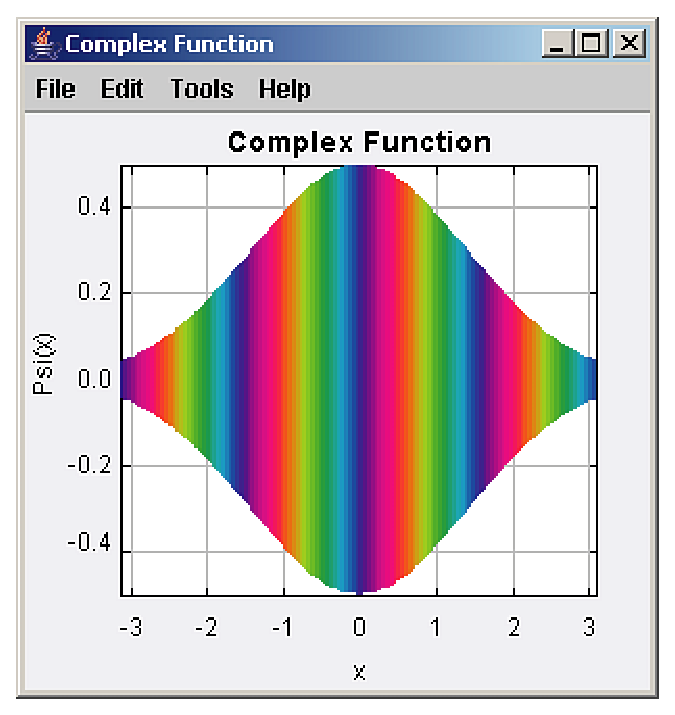
\includegraphics[scale=0.6]{phase}
\caption{\label{fig:phase}And here is your predicted phase diagram.}
\end{figure}


\section{Simulation Results}

And here, I show the simulation results, which fall into three categories, 1) the frequency falloff can be explained by heterogeneity in length, 2) the steady state effective viscosity matches the theoretical prediction in a range of parameter space, 3) the network tearing time drops as the effective viscosity drops to 0

We have implemented a solution to the discretized form of our model equations.  

\begin{figure}[h!]
\centering
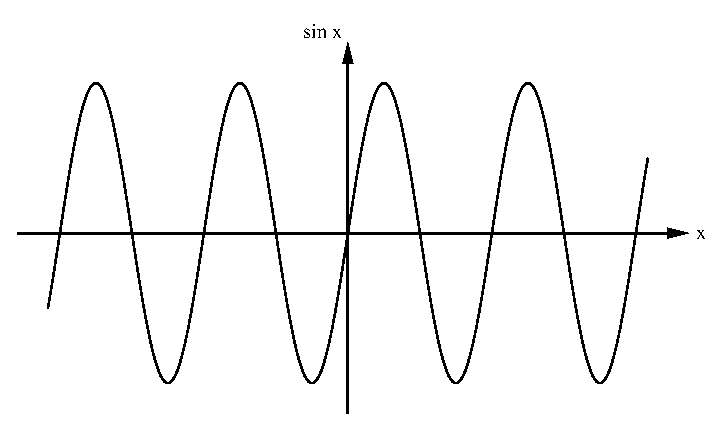
\includegraphics[scale=0.6]{sine}
\caption{\label{fig:sine}Show me a sine.}
\end{figure}

We can make figures bigger or smaller by scaling them. Figure~\ref{fig:sine}
has been scaled by 60\%.


\section{Simulation details}
And I think I'll probably include all the gory details of how my simulations work since I'll be wanting to have direct references to the code. 
\begin{verbatim}
double y0 = 10; // example of declaration and assignment statement
double v0 = 0;  // initial velocity
double t = 0;   // time
double dt = 0.01; // time step
double y = y0; // solved all problems
\end{verbatim}


\section{Discussion}

{\color{blue}{Finally I wax philosophical}},
{\color{green}{but}} {\color{cyan}{who is going pay for the ink?}}

\begin{thebibliography}{5}

\bibitem{latex}Helmut Kopka and Patrick W. Daly, \textsl{A Guide to
\LaTeX: Document Preparation for Beginners and Advanced Users} (Addison-Wesley, 2004), 4th ed.

\bibitem{website}Some useful links are
given at \url{<sip.clarku.edu/tutorials/TeX/>}.

\end{thebibliography}

\end{document}

\chapter{Additional information on pulse model}
\label{chap:morepulse}
\section{Motivation and experimental context}
In many systems, cortical flows are driven not by continuous contraction of active material, but by repeated rounds of pulsatile contraction.  While it was once believed that these pulsatile behaviors could be an emergent property of actomyosin contractility itself, it is now more probably suspected that 

It is still unclear why so many systems exhibit this type of behavior, it is nonetheless important to understand the origins of these behaviors and what differences may arise due to their presence or absence in a contractile system.  Therefore, we have begun exploring how to model both the upstream regulators that govern contractile systems as well as the downstream effects of coupling these to regulators to contractile flows themselves.

The majority of our data comes from the work of Francois Robin and Jon Michaux (cite).  They have shown that upstream of both actin and myosin is a separate pulsatile biochemical circuit consisting of a combination of positive and negative feedback between a pair of proteins called Rho and RGA as depicted in Figure \ref{fig:pulse_diag}.  For more information on the biochemistry of this circuit please see their paper (cite again).  

\begin{figure}[h!]
\centering
\includegraphics[width=0.5\hsize]{pulse/diagram.png}
\caption{\label{fig:pulse_diag}  Proposed reaction pathway for Rho excitability.}
\end{figure}

To explain the dynamics we attempted to build ordinary differential equation models of local variation in active Rho and RGA concentrations.  We found that many models are effectively equivalent at producing the qualitative results.  However, all of our models were fairly bad at producing robust pulsatile behavior once the models were constrained by parameter fitting to the data. 

\section{A model for pulsatile actomyosin accumulation in \textit{C. elegans} }

My first attempt at modeling involved a fair

I defined $\rho$ as the concentration of Rho and $r$ as the concentration of RGA, and generated association, dissociation and feedback parameters for the model. 

\begin{equation}
\label{eqn:rho_1}
	\frac{d\rho}{dt} = k_{on}^\rho \left( 1+k_{on}^{\rho\rho} \frac{\rho^n}{\rho_0^n +\rho^n} \right ) - (k_{off}^\rho + k_{off}^{\rho r} r) p
\end{equation}

\begin{equation}
\label{eqn:rga_1}
	\frac{dr}{dt} = k_{on}^{r \rho}\rho - k_{off}^r r 
\end{equation}

Next we can nondimensionalize the equation with $q=\rho/\rho_0$, $s=k_{off}^{\rho r}/k_{off}^r r$, and $\tau=k_{off}^r t$, and rename parameters for simplicity.

\begin{equation}
	\frac{dq}{d\tau} = k_q \left( 1+k_{qq} \frac{q^n}{1 +q^n} \right ) - (k_{off} + s) q
\end{equation}

\begin{equation}
	\frac{ds}{d\tau} = k_s q - s
\end{equation}

The null-clines are 

\begin{equation}
	s_q =\frac{k_q}{q} \left( 1+k_{qq} \frac{q^n}{1 +q^n} \right ) - k_{off} 
\end{equation}

\begin{equation}
	s_s = k_s q
\end{equation}

\begin{figure}[h!]
\centering
\includegraphics[width=0.5\hsize]{pulse/diagram_eq.eps}
\caption{\label{fig:pulse_diag}  Reaction pathway with labels for coefficients associated with feedback stregths.}
\end{figure}

\subsection{Analyzing parameter space of the model}

\begin{figure}[h!]
\centering
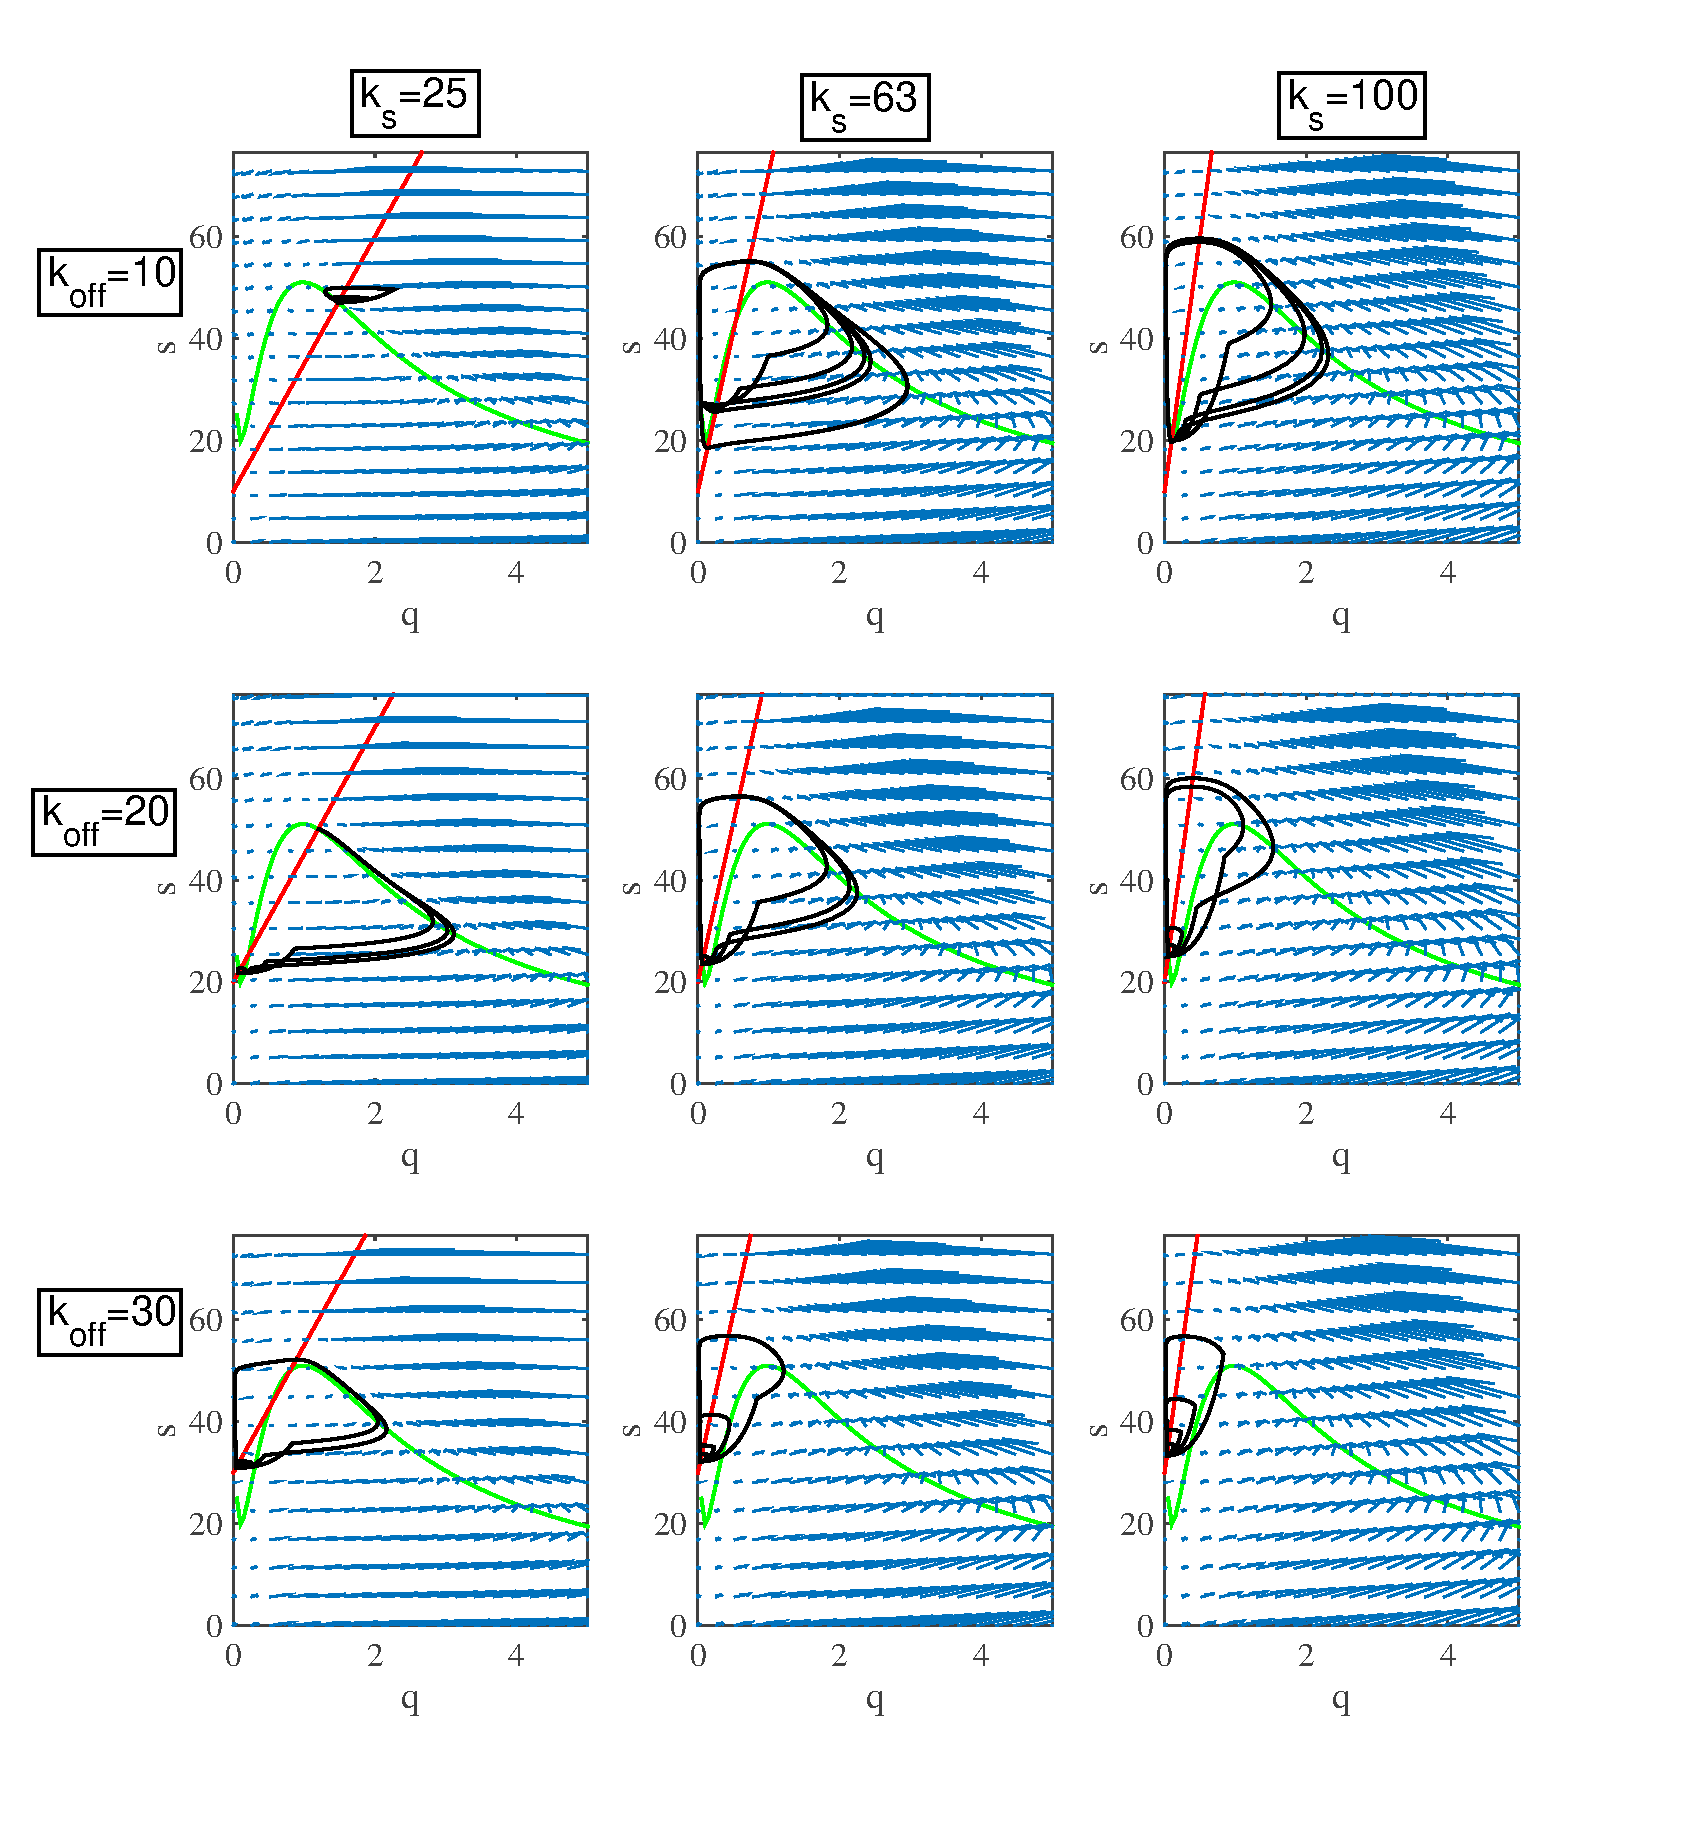
\includegraphics[width=\hsize]{pulse/phase_tester.eps}
\caption{\label{fig:pulse_fit}  Phase diagram of for $k_q=1$ and $k_qq=100$.}
\end{figure}

\begin{figure}[h!]
\centering
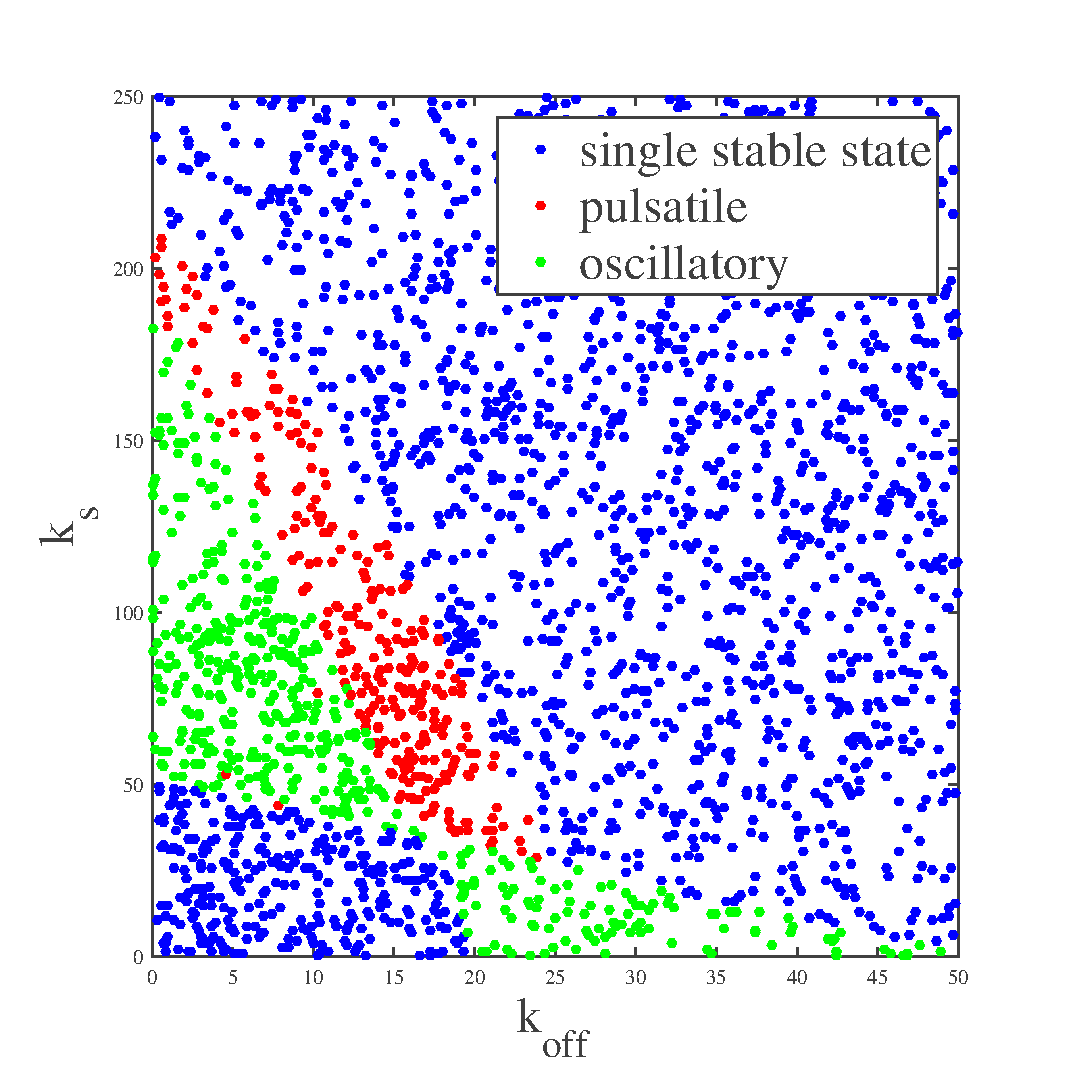
\includegraphics[width=\hsize]{pulse/k_phase.eps}
\caption{\label{fig:pulse_fit}  Phase diagram of for $k_q=1$ and $k_qq=100$.}
\end{figure}

\begin{figure}[h!]
\centering
\includegraphics[width=\hsize]{pulse/randomized_simulation.eps}
\caption{\label{fig:pulse_fit}  Phase diagram of for $k_q=1$ and $k_qq=100$.}
\end{figure}

\section{Simplified model and data fitting}

Although 

\begin{equation}
	\frac{dq}{d\tau} =\alpha \frac{q^n}{1 +q^n} - s q^k
\end{equation}

\begin{equation}
	\frac{ds}{d\tau} = \beta q^{(m-k)} - s
\end{equation}

These equations resulted in a family of models with different levels of feedback, depending on the values of $n$, $m$, and $k$.  I fit models with a variety of exponents and found that any model with $k\approx0$, $n>1$, and $m\approx2$ gave the best overall agreement with the greatest robustness.  

\subsection{Fitting techniques}
I used two different methods to fit the Rho and RGA data to determine the most appropriate model parameters.  The first required subsecting the data to fit only to regions where some parameters were presumable close to constant.  For example, as long as RGA concentration remained relatively small, the .


\begin{figure}[h!]
\centering
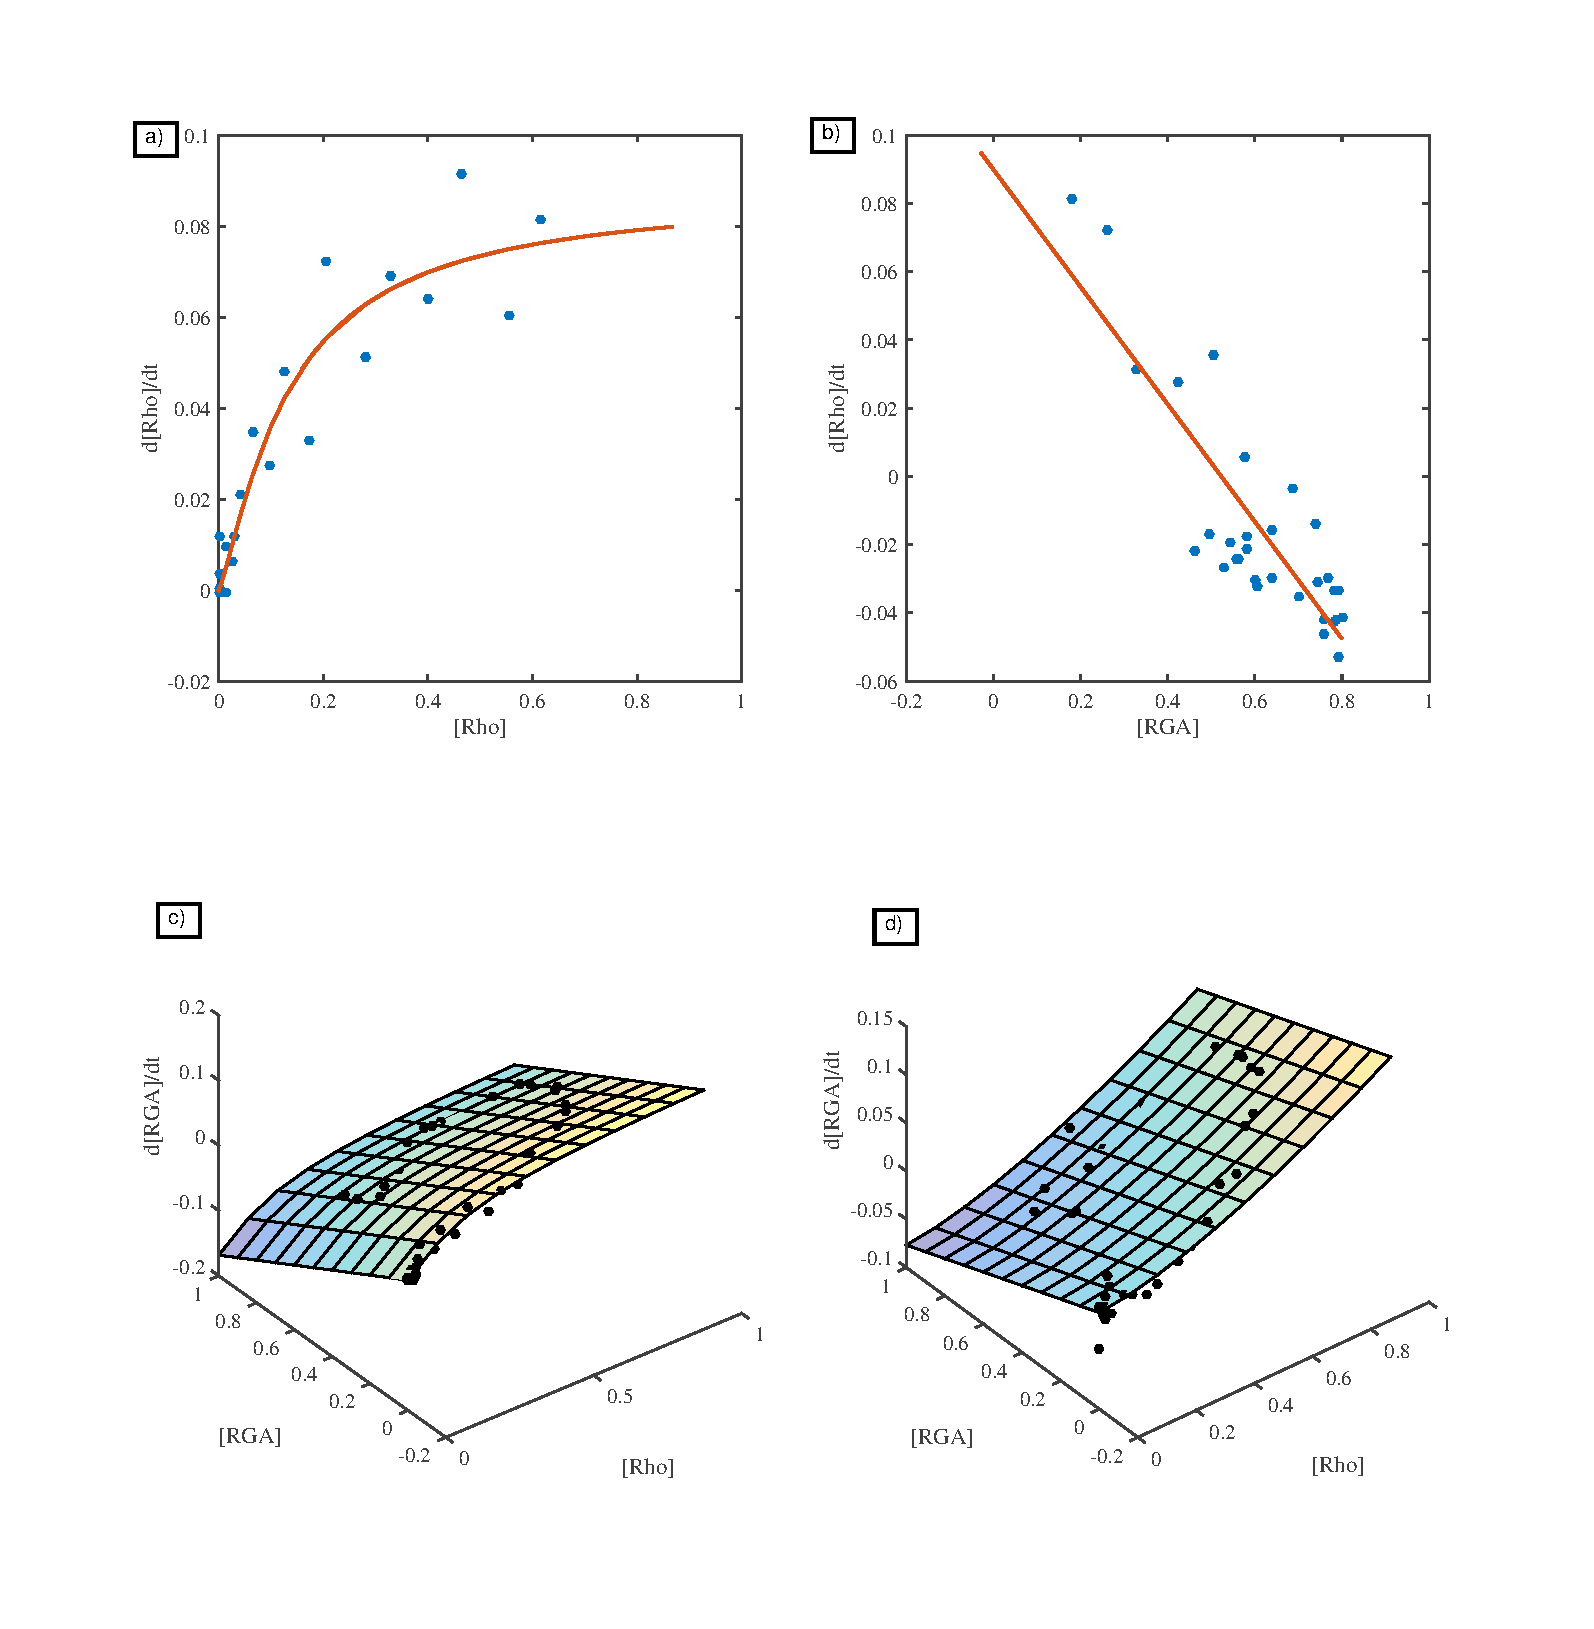
\includegraphics[width=\hsize]{pulse/fitting_plot.eps}
\caption{\label{fig:pulse_fit}  Multiple methods of fitting.}
\end{figure}

\begin{figure}[h!]
\centering
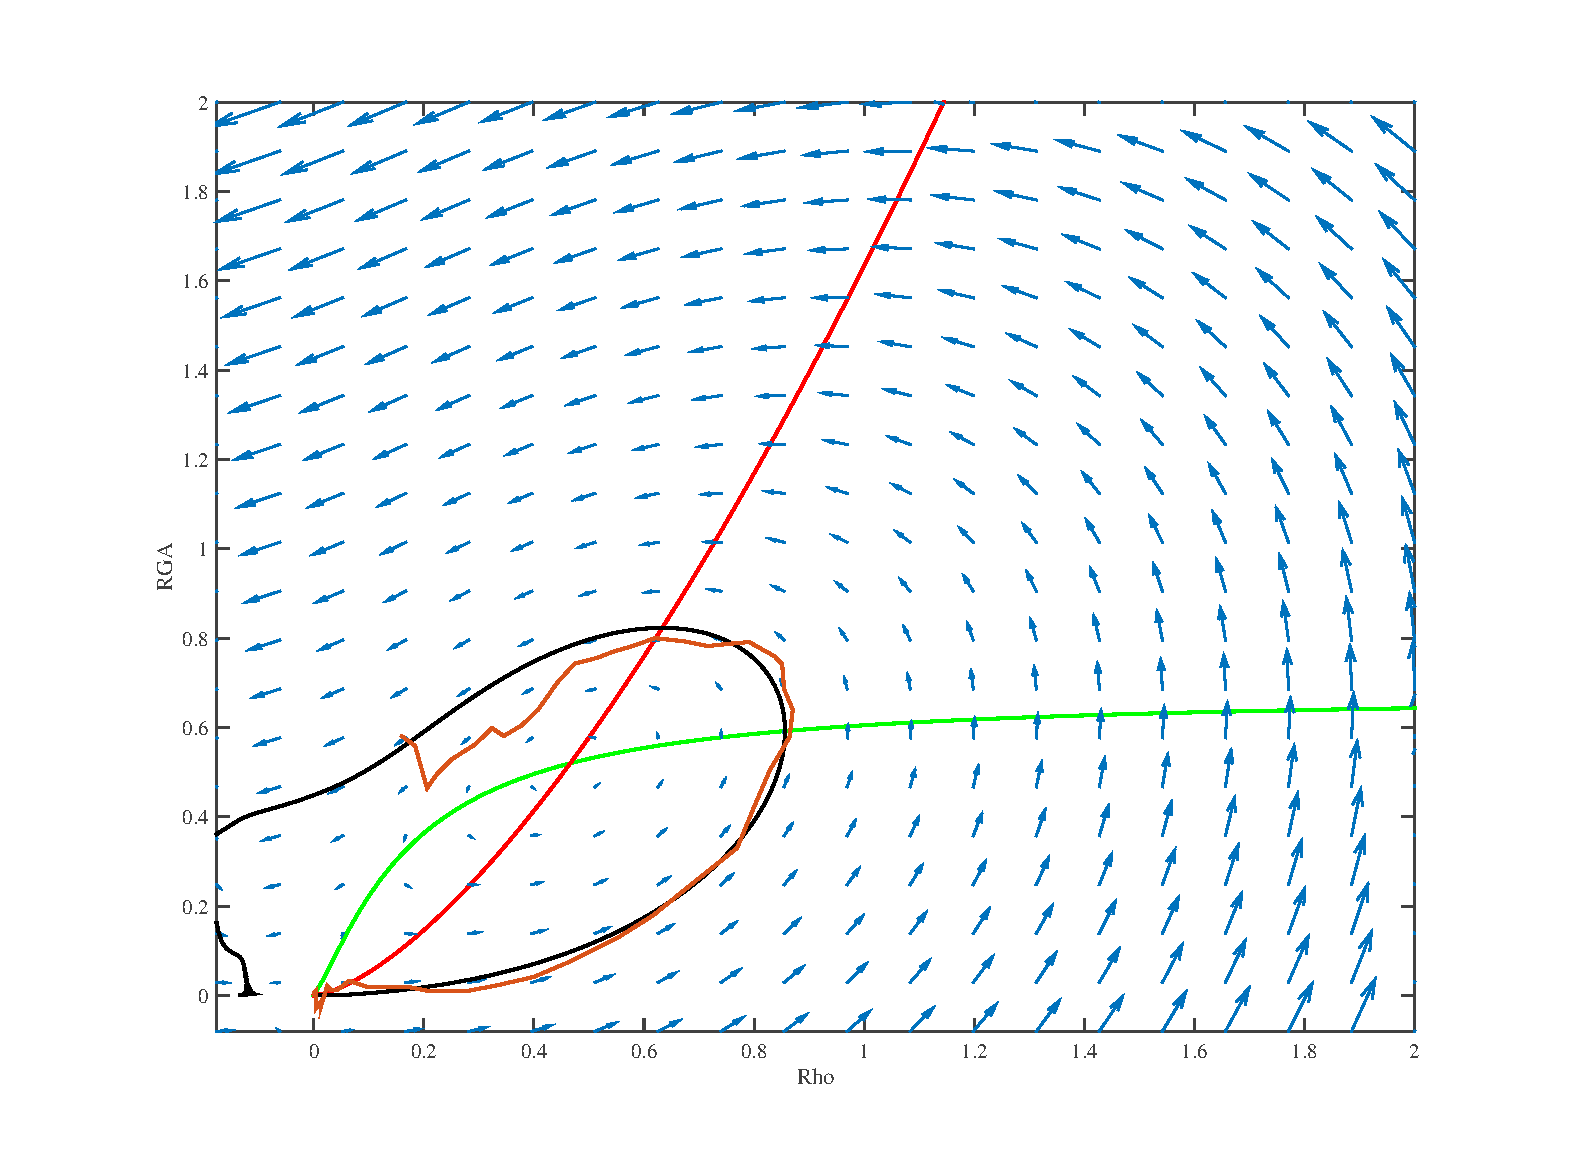
\includegraphics[width=\hsize]{pulse/simple_model_fit_phase.eps}
\caption{\label{fig:pulse_fit_phase}  Simulation results and fitted for phase diagram.}
\end{figure}

\begin{figure}[h!]
\centering
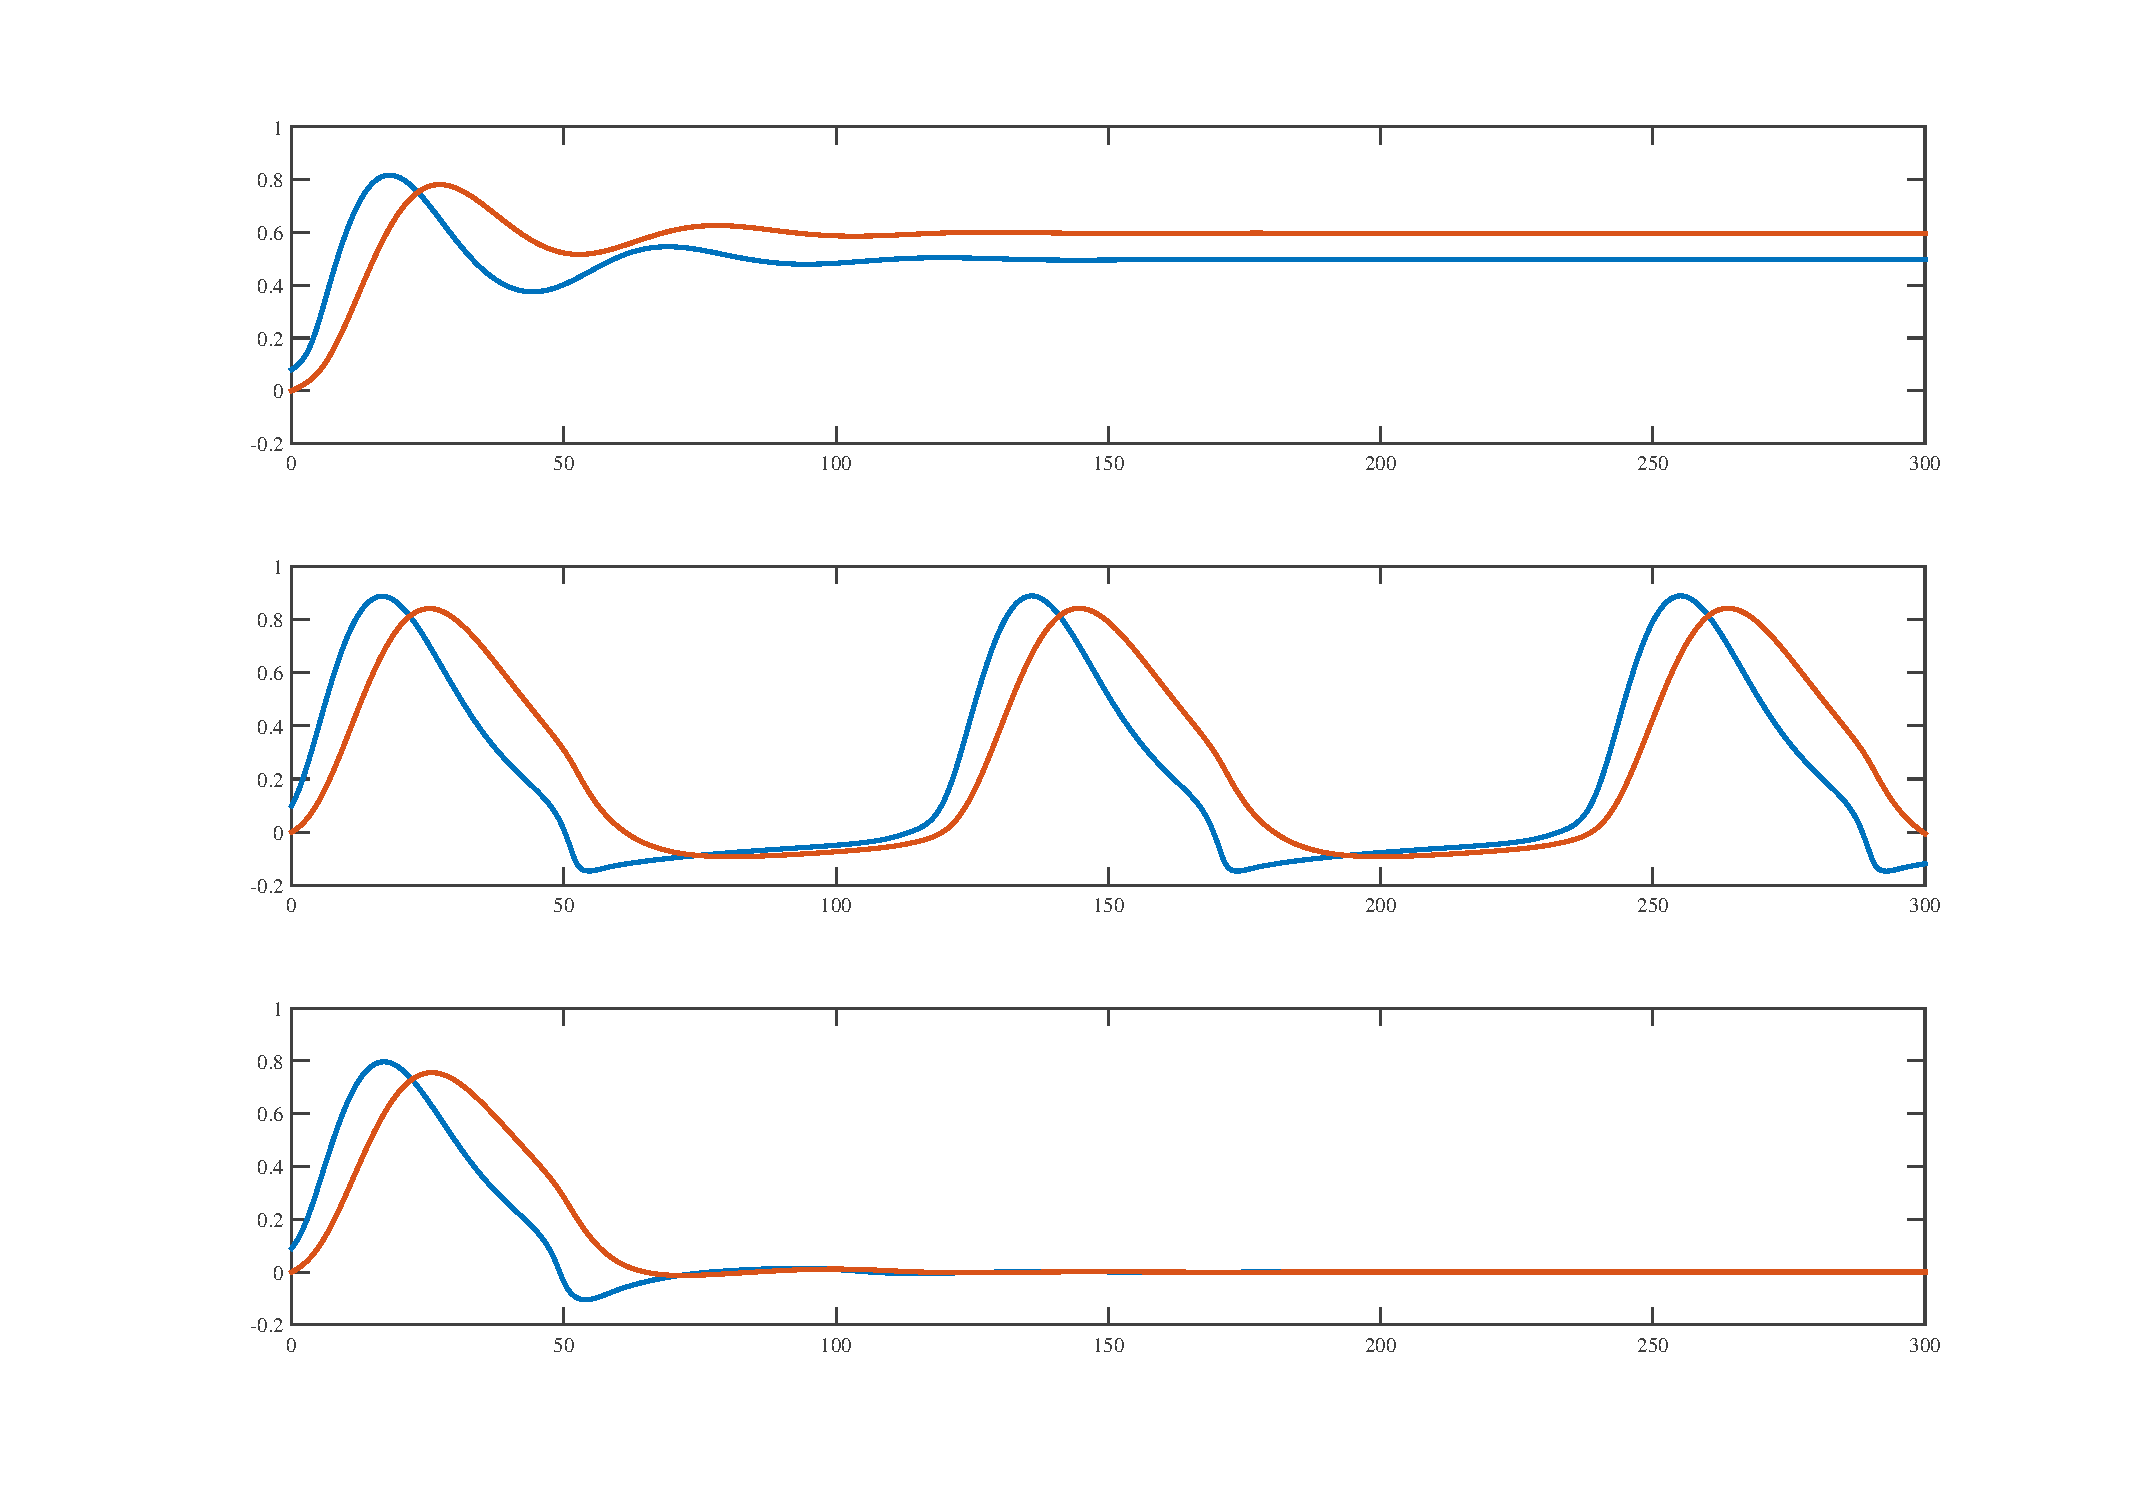
\includegraphics[width=\hsize]{pulse/model_compare.eps}
\caption{\label{fig:pulse_fit_phase}  Simulation results and fitted for phase diagram.}
\end{figure}

\begin{figure}[h!]
\centering
\includegraphics[width=\hsize]{pulse/model_profile.eps}
\caption{\label{fig:pulse_fit_phase}  Simulation results and fitted for phase diagram.}
\end{figure}




\section{Conclusion}
\begin{figure}[h!]
\centering
\includegraphics[width=\hsize]{pulse/final_fig.png}
\caption{\label{fig:pulse_final}  Final figure as it appears in Robin et al.}
\end{figure}
Ultimately, a model similar to \ref{eqn:rho_1} and \ref{eqn:rga_1} was utilized in the final paper in combination with at the 2D fitting routine outlined in Figure \ref{fig:pulse_fit}c,d.   In short, all models performed equally well (or poorly depending on perspective) at describing the qualitative features of the data, but none were very effective at generating a quantitative match.    We believe this is indicative of the need to perhaps extend to incorporating spatial effects in driving the dynamics of active material pulses.

Based on the theoretical results of [bois and the other one], we attempted to incorporate our upstream regulatory model into a 1D active fluid.  



\chapter{Reducing power consumption in High Performance Computing}


\section{Introduction}

Data centers in the US consume an estimated 91 billion kilowatt-hours yearly, equivalent to the annual output of 34 large coal-fired power plants.\cite{Delforge2014} These same estimates show that only 6-12\% of the electricity is used for powering servers while the rest is used to keep machines idling, wasting resources and money in the process. Data center electricity is not inexpensive, costing American businesses \$13 billion annually in electricity bills.\cite{Delforge2014} Because cost is a strong motivating factor for businesses and universities, we consider data center energy efficiency in the context of cost savings for data center operations. \\

\begin{figure}[t]
	\begin{center}
		\includegraphics[scale=0.38]{edeals/pwr_model_ins}
		%		\begin{picture}(300,150)(0,200)
		%		\put(-15,-30){\special{psfile = fig1.ps hscale = 50 vscale = 50}}
		%		\end{picture}\\
	\end{center}
	\caption{Average core usage for a 244 node shared HPC partition in the Midway cluster. Insert shows usage statistics histogram.}
	\label{prw_model_ins}
\end{figure}

Demand response (DR) programs provide incentives to induce dynamic management of customers’ electricity load in response to power supply conditions, for example, reducing their power consumption in response to a request from the utility.\cite{7039172} Anita can you add something around here that points out how demand response also increases the “sustainability” of the datacenter beyond just cost reduction.Many energy providers have Voluntary Load Response (VLR) programs, which encourage commercial consumers to reduce power demands during peak periods, such as particularly hot summer days. Participants are given between one and four hours’ notice of a request to shed some of their electric load, with two and eight hours of participation and the expectation to shed at least 10 kilowatts. We are interested in exploring more active ways in which to participate in electricity demand response programs while impacting the users minimally.   \\

In many university data centers, a significant portion of the data center is dedicated to high performance research computing which is typically Tier 1. While these jobs take longer periods of time to complete, they are less time sensitive and more flexible than systems which support core business functions such as the university's email.  We wish to use the flexibility in scheduling of these jobs to reduce energy consumption of university data centers during periods of peak energy demand. \\  

As shown in the example core usage data of Figure \ref{prw_model_ins}, although the typical average usage during the school year is a fairly standard 80\%, the averaged workload can fall to 65\% of full capacity in the hottest summer months from June to September. These months also present the period of greatest electricity demand due largely to increased usage of air conditioning. This presents a valuable opportunity to potentially curtail electricity use in demand response scenarios by shifting load off of the peak periods of energy price.  Toward this aim, this paper is our attempt to estimate the economic savings, feasibility, and any potential user impact from full or partial cluster shutdown during periods of increased energy demand.


\subsection{Alternative Demand Response Options in Data Centers}

Although we focus on load shifting for our study, we wish to point out prior work on alternative strategies for demand response. \\

\textbf{Facility changes} A study by Lawrence Berkeley National Laboratory (LBNL) found that 5\% of the data center load can typically be shed in 5 minutes and 10\% of the load can be shed in 15 minutes without changes to how the IT workload is handled, i.e., via temperature adjustment and other building management approaches\cite{Ghatikar2012}. Most data centers have local power due to a backup generator, which could also be used to absorb some load during peak time \cite{Liu2013}. More recently, methods of energy storage have been proposed\cite{Narayanan2014} in which UPS batteries are re-purposed for provisioning during periods of peak demand in addition to their primary purpose of backup power. However, these methods all entail manual intervention, with close monitoring and control.

\textbf{Power capping} is a strategy by which to run data center equipment within a set of constraints which assume the electricity draw for the data center as a whole cannot grow any larger. Some examples of this include and turning off or constraining CPU/GPU power consumption to values below the CPU Thermal Design Power (TDP) value, which requires less voltage. Many equipment manufacturers - including IBM, Intel and AMD - have implemented power capping technology that can be monitored at the processor level and applied at the rack level. One approach to power capping is Dynamic Voltage/Frequency Scaling (DVFS). However, as noted by Roundtree\cite{Roundtree2012}, no machine in the Top 500 list of supercomputers makes use of DVFS to save power or energy since the performance impact and the amount of power and energy saved was highly application dependent. Power capping doesn’t necessarily equate to energy efficiency nor cost savings.

\textbf{Schedulers} Zhou et al\cite{Zhou2014} present a method for power-aware scheduling by using a combination of a scheduling window and 0-1 knapsack model, which shows promise. However, since SLURM is our scheduler, we decided to focus solely on SLURM. Bodas et al\cite{Bodas2014} demonstrate an integration of power capping into a power-aware scheduler, with the overall goal of maintaining average system power within a budget. Their work demonstrates that SLURM’s auto mode can be used to maximize available power.  

\begin{figure}[t]
	\begin{center}
		
				\begin{picture}(300,100)(20,200)
				\includegraphics[scale=0.50]{edeals/ray_fig}
				\end{picture}\\
	\end{center}
	\caption{Energy monitoring framework.}
	\label{ray_fig}
\end{figure}


\section{Problem Statement}

Can load shifting of high performance computing tasks save universities money in energy demand response scenarios?  To explore the relative costs of implementing load shifting in demand response scenarios, we have expressed the problem by modeling total dollar cost.  We wish to use this framework to explore the optimization of price in the presence of various data center usage statistics and price fluctuation schemes.

\subsection{Modeling Energy Costs}

We generate a model total cost function composed of a fixed cost for purchasing and maintaining nodes plus a variable cost dependent on data center power usage and energy prices.  We wish to minimize the cost function

$$C = p_n T n_{max} + \int_0^T dt \cdot p(t)\left (n(t)u(t)+ u_w \frac{\Delta n(t) }{\Delta t} \right )  $$

where $p(t)$ is the price of power at time $t$, $0<n(t)<n_{max}$ is the number of running nodes, $u(t)$ is the average node power usage, $u_w$ is the wasted power from turning on a node, $p_n$ is the amortized lifetime cost of purchasing a node, and $n_{max}$ is the total number of nodes in the cluster.  

Based on our cluster usage statistics, we approximate that compute cycles are roughly interchangeable and that the main determiner of power usage is simply the CPU utilization of the node. In this case, node power usage takes the form

$$u(t) = u_0 + u_v \cdot r(t)$$

where $0<r(t)<1$ is the fraction of CPU usage, $u_0$ is the cost of an idling node and $u_v$ is the variable cost for doing $r$ work on a machine.

We wish to minimize the cost function $C$ subject to the constraint that the sum of the submitted CPU cycles, $S$, are all completed after a period T.

$$\int_0^T dt \cdot n(t)r(t) = S$$

\begin{figure}[t]
	\begin{center}
		\includegraphics[scale=0.55]{edeals/usage_viz4}
		%		\begin{picture}(300,150)(0,200)
		%		\put(-15,-30){\special{psfile = fig1.ps hscale = 50 vscale = 50}}
		%		\end{picture}\\
	\end{center}
	\caption{Diagram of job scheduling during a four node temporary shutdown experiment. Each colored rectangle displays the execution time of a single LAMPPS test job running for approximately 5 minutes.}
	
\end{figure}

\begin{figure}[t]
	\begin{center}
		\includegraphics[scale=0.55]{edeals/power_viz}
		%		\begin{picture}(300,150)(0,200)
		%		\put(-15,-30){\special{psfile = fig1.ps hscale = 50 vscale = 50}}
		%		\end{picture}\\
	\end{center}
	\caption{Total power consumed during experiments where variable numbers of machines were shut down during simulated peak pricing.}
	\label{power_viz}
\end{figure}

\subsection{Response to a Temporary Price Spike}

In particular, we wish to use this framework to determine how to run our data center in the situation where every $T$ days, we see a "price spike" from $p_0$ to $p_s$, lasting time period $t_s$.  This condition is highly similar to the one facility managers face when utility provides impose usage tariffs during peak energy demand periods.

In this situation, the number of running machines will change stepwise between a high number of running machines, $n_H=n_{max}$, and a low number of running machines, $n_L$, and a high and low CPU utilization $r_H=1$, $r_L$, with a corresponding $u_H$ and $u_L$ as defined above.  The high usage will occur during the cheap energy supply, and the low usage will occur during the price spike.  Therefore we can rewrite our cost function as 

\begin{equation}
	C = p_n n_H T + p_0 (u_0 + u_v) n_H (T-t_s) + p_s (u_0 + u_v r_L) n_L t_s + p_0 u_w (n_H-n_L)
\end{equation}

with the constraint

\begin{equation}
n_H (T-t_s) + n_L r_L t_s = S
\end{equation}

Inserting the constraint into our cost function to replace $r_L$ yields 

\begin{equation}
C = p_s u_v S + n_L \cdot( p_s u_0 t_s - p_0 u_w t_w) + n_H \cdot (p_n T + p_0 u_w t_w -(\Delta p u_v - p_0 u_0)(T-t_s))
\end{equation}
where we've introduce the price difference, $\Delta p = p_s - p_0$.

We can analyze the change in costs as a function of $n_L$ and $n_H$ to determine the optimal cluster setup for known variables, $t_s$, $p_s$, $p_n$, $p_0$, $u_0$, $u_v$, and $u_w$. 

From this analysis, whenever $ p_s u_0 t_s < p_0 u_w t_w$, the cost of powering off nodes exceeds the cost of running those nodes idle so $n_L = n_H$ and $r_L = S/n_H t_s - (T-t_s)/t_s$. Otherwise powering off nodes saves money so the nodes that remain on run at full capacity $r_L = 1$, and $n_L$ is minimized subject to constraints giving $n_L = S/t_s - n_H(T-t_s)/t_s$.

If we can freely choose $n_H$ to optimize cost, then whenever $(\Delta p u_v - p_0 u_0)(T-t_s) > p_n T + min(p_0 u_w t_w,p_s u_0 t_s)$, we would increase $n_H$ (i.e. buy more machines) until all the work is done during the cheap energy period. Therefore $n_H = S/(T-t_s)$ and either $n_L$ or $r_L$ is $0$.  Otherwise, the cost of new machines is more than any cost savings achieved from exploiting the price difference, and we would simply ignore the price spike (i.e. set $n_H = n_L = S/T$ and $r_L = 1$).

% you can also use the wonderful epsfig package...
\begin{figure}[t]
	\begin{center}
		\includegraphics[scale=0.55]{edeals/down_v_pow}
		%		\begin{picture}(300,150)(0,200)
		%		\put(-15,-30){\special{psfile = fig1.ps hscale = 50 vscale = 50}}
		%		\end{picture}\\
	\end{center}
	\caption{Energy usage of test cluster during partial shutdown experiments.  Solid lines indicate power usage during the shutdown, while dashed lines indicate power usage after returning to full operation.}
	\label{down_v_pow}
\end{figure}

% you can also use the wonderful epsfig package...
\begin{figure}[t]
	\begin{center}
		\includegraphics[scale=0.55]{edeals/down_v_wait}
		%		\begin{picture}(300,150)(0,200)
		%		\put(-15,-30){\special{psfile = fig1.ps hscale = 50 vscale = 50}}
		%		\end{picture}\\
	\end{center}
	\caption{Maximum (solid) and mean (dashed) job wait times during partial shutdown experiments.}
	\label{down_v_wait}
\end{figure}

\section{EDEALS: Electricity Demand-response Easy Adjusted Load Shifting}

For a data center manager to use the above model to determine their cost savings, they must collect and analyze usage and power data on their system.  We have built a cluster data processing pipeline, EDEALS, to assess the magnitude of potential savings available from a full or partial cluster shutdown.  We combine SLURM job scheduling, node level IMM power and usage metrics, and cabinet level CDU measurements to determine the optimum magnitude of demand response cluster shutdowns.  

Here we describe our data center instrumentation, so that we ensure accurate measurements of performance of the workload management system and HPC cluster alone without the influence of extraneous components. Since our focus is the HPC cluster and SLURM manager, we need to ensure those components alone affect the reduced data center utility bill.  As depicted in Figure \ref{ray_fig}, we take measurements at the core, node, rack, and cabinet level.  These data are combined to detect power losses at each step and to determine the correlation between the power measurements at the machine level and the true power draw at the facility level.

Combining this data with electricity pricing statistics from utility managers allows system administrators to determine when and by how much to reduce their power usage to save money.  We have built a set of scripts particular to our system to implement machine level power down in response to predicted energy peaks.  At the end of the peak energy period the machines automatically reboot and are added by to SLURM’s available server pool.  At this time, these power cycling scripts are manually executed by system administrators after evaluation of the likelihood of near-term energy demand peaks.  However, as more data centers begin to implement smart metering, it will become possible to automate load shifting in response to real-time energy pricing indicators.  We look forward to continuing this as future work.





\section{Small-Scale Evaluation of EDEALS}

To test our load shifting scheme, we launched a series of small-scale experiments on a 6 machine test cluster using SLURM batch management system to schedule jobs. We wished to compare the energy savings and job wait times during a full or partial cluster shutdown in response to an energy price spike.

\subsection{Experimental Setup}

We measured the total energy use over a 3.5 hour window of which the first 30 minutes comprised a partial cluster shutdown, followed by a 15 minute powerup routine. We explored the impact of shutting down between one and all six nodes during the 30 minute window. The shutdown was carried out by fully powering nodes off.  We compared this to the energy usage without the partial shutdown.

Identical sample jobs were submitted to the cluster via SLURM scheduler at a constant rate to set the average cluster usage to approximately 55\%, 60\%, 65\% and 75\% capacity.  We used custom state control commands to set the power states of individual machines in the test cluster.  The SLURM scheduler automatically shifted queued jobs to run on the available machines, as shown in the example job schedule displayed Figure \ref{usage_viz} from a four node shutdown experiment. We used our EDEALS data analysis pipeline to measure the changes in energy usage and job wait time in the queue.

\subsection{Evaluation of Model Parameters}

Importantly, EDEALS allowed us to determine appropriate power parameters, $u_0$, $u_v$, and $u_w$ for both our test rack as well as a larger partition of the University of Chicago's Midway production cluster.  Figure \ref{pwr_proc} shows the measured relationship between CPU utilization and energy usage as determined from the machine level IPMI metric data.


\begin{figure}[t]
	\begin{center}
		\includegraphics[scale=0.55]{edeals/pwr_proc}
		\includegraphics[scale=0.55]{edeals/pwr_proc_c}
		%		\begin{picture}(300,150)(0,200)
		%		\put(-15,-30){\special{psfile = fig1.ps hscale = 50 vscale = 50}}
		%		\end{picture}\\
	\end{center}
	\caption{Power data for test cluster (top) and production cluster (bottom) nodes in presence of variable usage. The slope and intercept of the line are used to determine $u_v$ and $u_0$ respectively. }
	\label{pwr_proc}
\end{figure}

\begin{figure}[t]
	\begin{center}
		\includegraphics[scale=0.55]{edeals/ipmi_v_cdu}
		%		\begin{picture}(300,150)(0,200)
		%		\put(-15,-30){\special{psfile = fig1.ps hscale = 50 vscale = 50}}
		%		\end{picture}\\
	\end{center}
	\caption{Comparison between node level IPMI measurements and rack level CDU measurements. Best fit shows the model relationship used to convert IPMI data to estimated total power draw.}
	\label{ipmi_v_cdu}
\end{figure}

To account for losses not measured at the IPMI level, we compare the sum IPMI power usage to the rack level power monitoring.  This comparison revealed a correction factor of 1.25 between the IPMI measurement and the total rack level energy draw.  Using this corrected model, we were able to predict power consumption at the CDU level via CPU utilization under variable scheduler loads.

\subsection{Relative Energy Savings and Max Wait Times}

Our test cluster provided us with an important baseline in determining the effectiveness of a partial shutdown in reducing energy usage. As shown in Figure \ref{power_viz}, the total power draw from the test cluster was reduced dramatically during the shutdown period, and then returned to its baseline level.  

These experiments were repeated with different job submission rates such that the average CPU usage varied from 55\% to 75\%.  As shown in Figure \ref{down_v_pow}, the partial shutdowns reduced the total energy usage as measured at the CDU level.  Not surprisingly, the power usage during cluster shutdown for all usage levels converged to roughly the same value at the point where all remaining operational machines reached full capacity. Interestingly, the energy savings did not appear to be perfectly directly proportional to the fraction shut down.  In particular, there was residual energy use associated with our machine's low power state even when the cluster was entirely shut down.   

We also measured the difference between job submission and start time, as depicted in Figure \ref{down_v_wait}.  As one would expect, both mean and max wait times increased as the shutdown fraction grew and the effect was more pronounced when the cluster usage was higher.  However, we were pleasantly surprised to find that max wait times topped out at 45 minutes, which was the duration of the entire cluster down period.  This indicates that SLURM doesn't add too much additional overhead, and therefore, the worst-case user wait times would not exceed the total period that the cluster was shut down.

\section{Conclusion: Implication for An Operational HPC Datacenter}


In an HPC datacenter, the variable cost to supply electricity to a facility can be decomposed into both a nominal cost per kilowatt-hour and a procurement cost from the supplier.  Some suppliers impose a substantial procurement tariff based on electricity usage during the five, two hour long periods of highest demand in a year.  In this scenario, the savings of load shedding can be orders of magnitude higher than the nominal price per kilowatt-hour.  We estimate that by curtailing 1MW, 8 times per year, we can expect an annual savings of approximately \$100K, which in our case was roughly a 7% cost savings.  Approximating that the 8 curtailment days are roughly spread out over the 4 month period from June to September, we arrive at the system parameters listed in Table \ref{params}.



Combining these values with the power usage measurements from our production cluster, we can extrapolate the yearly savings based on fractional shutdowns of the data center.  In addition, using the wait time statistics from our test cluster we can also estimate the worst-case impact on user wait-times that these cluster shutdowns will incur.  We display this information in Figure \ref{final}, as a function of the fraction of the cluster that we would be theoretically willing to shut down.

\begin{figure}[t]
	\begin{center}
		\includegraphics[scale=0.5]{edeals/final}
		%		\begin{picture}(300,150)(0,200)
		%		\put(-15,-30){\special{psfile = fig1.ps hscale = 50 vscale = 50}}
		%		\end{picture}\\
	\end{center}
	\caption{Estimated savings from partial cluster shutdowns. }
	\label{final}
\end{figure}


\begin{table}[]
	\centering
	\label{my-label}
	\begin{tabular}{|l|l|l|l|}
		\hline
		\textbf{$T$} & \textbf{$t_s$} & \textbf{$p_0$} & \textbf{$p_s$}  \\ \hline
		360 hr & 2 hr & \$0.03/kWh  & \$6.5/kWh    \\ \hline
	\end{tabular}
	\caption{Model parameters estimated for medium scale HPC datacenter.}
	\label{params}
\end{table}

\section{Acknowledgments}

Special thanks goes out to Brandon for all his work getting our test cluster set up as well as for his useful input on machine pricing information.  We also wish to thank Matt Beach for his invaluable knowledge on energy pricing mechanisms and university power plans.  Finally, we wish to thank Dr. Birali Runesha for his support in carrying out this project.

\section{Availability}

On our Github, we have provided all data collection scripts, analysis routines, and experimental setups, as well as detailed calculations and optimization methods for other price models.  

\begin{center}
{\tt https://github.com/rcc-uchicago/datacenter}
\end{center}








\chapter{Source Code and Documentation}
\section{Documentation of Simulation Framework}




\subsection{Simulation Code}
\lstinputlisting{docu/simulation/activnet_gen.m}


\section{Practical Implementation of Model Framework}

Although the prior description is useful for communicating the mathematical principles underlying my modeling framework, I also want to provide a practical explanation of the logic of the code structure.  This will help to clarify the implementation details that may be ambiguous in the above formulation and make it easier for others to approach and modify my code.

The simulation code is entirely built on top of MATLAB's ode solving functions.  Therefore, at the highest level, the entire simulation framework simply boils down to providing functions to define the ode's left and right hand side, along with the initial conditions for the system.  However, because MATLABs solvers do not allow discontinuities, discontinuous filament recycling events cannot be implemented directly in the ODE.  Effectively, it is necessary to stop the simulation solver at fixed times, reset some subset of filaments, and restart the solver with the new state every time a turnover event happens.


In the following sections, I'll walk through the code's logic in more detail, emphasizing the packages and files that modularly summarize the core functions.  First I will begin with an explanation of the command line interface used to set model parameters and deploying simulations.


\subsection{Launching simulations from the command line}



The activnet package includes a function called activnet\_gen.m, which can be used to launch simulations on any MATLAB system.  The following is the documentation of the parameters passed to this function.

\begin{verbatim}
function p = activnet_gen(zet,L,mu,kap,lc,xi,ups,phi,psi,
                          r,sig,Dx,Dy,Df,Dw,ls,lf,tinc,tfin,nonlin)
% generates an active network simulation and prints node positions
% at time steps.  Parameters are defined as follows:
%
%   zet - medium viscosity
%   L - length of the filament
%   mu - compressional modulus of the filament
%   kap - bending modulus of a filament if ls<L
%   lc - average distance between filament overlaps
%   xi - frictional resistance between two overlapping segments
%   ups - motor force at filament overlaps
%   phi - fraction of overlaps that receive a motor force
%   psi - spatial variation in motor force 
%         (if external force applied, psi sets the periodicity of 
%          force application, and psi<0 sets square wave.)
%   r - recycling rate
%   sig - applied stress in the x direction applied at Df*Dx
%         (sig<0 sets stress to be applied in y direction)
%   Dx - x-dimension of domain
%   Dy - y-dimension of domain
%   Df - position at which external force is applied
%         (if Df<0, also position in x dimension where network stops )
%   Dw - width of window in x-dimension where forces/constraints are applied
%   ls - length of filament segments
%   lf - length of force falloff at end of filament (for continuous forces)
%   tinc - time increment to return solutions 
%          (will be decreassed automatically if r is too large)
%   tfin - end time of simulation
%   nonlin - nonlinear factor by which to make filament stiffer by extension
%            (if nonlin<0, then add spacing so filaments do not reach edge)
\end{verbatim}

These parameters will be explained in more detail below, but here I'll provide a brief practical explanation for their use in setting up simulations.  The parameters \texttt{zet}, \texttt{L}, \texttt{mu}, \texttt{kap}, \texttt{lc}, \texttt{xi}, \texttt{ups}, \texttt{phi}, \texttt{r}, \texttt{sig}, \texttt{Dx}, and \texttt{Dy} are defined in the mathematical methods section above as $\zeta$, $L$, $\mu_c$, $\kappa$, $l_c$, $\xi$, $\upsilon$, $\phi$, $1/\tau_r$, $\sigma$, $D_x$, and $D_y$, respectively. The parameter \texttt{nonlin} is used to internally calculate the extensional modulus $\mu_e = \texttt{nonlin} \times \mu_c$ (i.e. if \texttt{mu} is 1 and \texttt{nonlin} is 100, then $\mu_c=1$ and $\mu_e=100$).  The parameter \texttt{psi} is used to generate a spatial gradient in internal activity or temporal periodicity if an external force is applied. The spatial gradient is linear with a maximum at the center of the domain.  The parameter \texttt{Df} defines the x-position where any external stress will be applied (i.e. stress is applied at \texttt{Df}x\texttt{Dx}).

All of these terms are positive by definition so setting certain terms negative is used to trigger certain behavior in the simulation environment:
\begin{itemize}
	\item  Setting $\texttt{mu} < 0$ enables the extensional spring to be different than the compressive.
	\item  Setting $\texttt{sig} < 0$ causes the external stress to be applied in the y direction rather than the x direction, resulting in shear stress simulations.
	\item Setting $\texttt{nonlin} < 0$ results in space being added to the edge of the domain so that no filaments intersect with the boundaries of the simulation, allowing the network to undergo unconstrained contraction.
	\item Setting $\texttt{psi} < 0$ results in oscillating positive and negative stressed being applied to the network (as opposed to a sinusoidal pattern regularly).
	\item Setting $\texttt{Df} < 0$ will cause the rightward edge of the initially generated network to end at the location where the force is applied.
\end{itemize}
   
The parameter \texttt{ls} sets the segment size of the filament.  Theoretically this segment size is very small (the size of a single actin monomer perhaps), but for computational reasons this value is set much larger.  The parameters \texttt{Dw} and \texttt{lf} set the regions over which forces will "fall off" for the domain and individual filaments, respectively.  These are just there to ensure there are no discontinuous changes in the ODE equation as filaments move around, and should be set to some smallish number, like $0.05$, but shouldn't effect the results too much overall.  Finally, \texttt{tfin} and \texttt{tinc} set the end time of the simulation and the timesteps at which to print results, respectively.  The program will automatically shrink \texttt{tinc} if the recycling rate, \texttt{r} is large enough that manual position updates must occur on timescales smaller than \texttt{tinc}.


To run a simulation with an external stress the following code could be used.

\begin{verbatim}
activnet_gen(0.001, 1, -0.01,  0,  0.8, 10, 0, 0, 0, 
             0, -0.002, 20, 4, -0.33, 0.05, 1, 0.025, 1, 10000, 100)
\end{verbatim}

To run a simulation with internal filament activity the following code could be used.

\begin{verbatim}
activnet_gen(0.001, 5, -0.01,  0,  0.3, 10, 0.1, 0.25, 0, 
             0.001, 0, 25, 25, 0.5, 0.05, 5, 0.025, 1, 10000, -100)
\end{verbatim}

Both of these have nonlinear filament extension because the third argument (\texttt{mu}) is less than 0.  The results will be printed to the MATLAB console.

The currently deployed package can also be used to launch simulations on any linux system with MATLAB 2014b or the MATLAB 2014b Compiler Runtime installed (you will need to have a \$MATLAB environt variable enabled.  Please contact your sysadmin.).  In addition, the package can be recompiled on any system running MATLAB to create a new deployment that will be (see the README.txt file for more information about deployment).  

\begin{verbatim}
./run_activnet_gen.sh $MATLAB 0.001 1 -0.01  0  0.8 10 0 0 0 0 
         -0.002 20 4 -0.33 0.05 1 0.025 1 10000 100 > output.file
\end{verbatim}






\subsection{ODE Wrapper functions }

As demonstrated above, the initialization and launch of the simulation takes place using the function activnet\_gen.m.  This function is quite simple. It just ensures proper input parameters, builds a randomized network of filaments, prints the network node positions, and then calls the function activnet.m to compute the simulation results.  From there, activnet.m takes care of pausing solvers to update filament position for recycling as well as choosing between solvers depending on the type of problem being solved.  

\subsubsection{Generating Initial Conditions}

To select the number of filaments, $N$, to generate using the input parameters, we use the approximating formula $N \approx floor(2*Dx*Dy/lc/L)$.  This formula is derived from the tiling of a $Dx \times Dy$ domain with lines of length $L$ and spacings between lines $lc$.  This diverges from the exact number of filaments needed when $L/lc$ is small, but we ignore this discrepancy because we mostly operate in the regime where $L/lc>10$.

In most cases, the network should be assembled such that the domain is filled entirely in the y dimension ($y=0$ and $y=Dy$) and filled to the left edge ($x=0$) and up to the position $x=Dp*Dx$ in the in the x-dimension.  However, in the case that the parameter \texttt{nonlin} is less than 0, we set the initial conditions such that there is an empty space of size $0.2 Dx$ and $0.2 Dy$ at the x and y boundaries.  

To keep our density the same we should adjust our calculation of $N$ above, however, in the current implementation this adjustment is not made. This is a known bug that was corrected for after-the-fact in the publication. 


\subsubsection{Choosing between active and driven simulations }

During development I noticed that there were some cases where I could skip certain sections of the computation to speed up integration of the ODEs.  In particular, when there is no internal forces generated by filament activity, the right hand side of the differential equation is easier to compute (see below).  Therefore, in any situation where internal activity is set to 0, we use the more efficient code.  The activnet.m code makes this decision by determining if there is "pulling" of filaments rather than internal force generation.  

\begin{verbatim}
pull = (isempty(nu)&&sig~=0) 
\end{verbatim}

In this case it runs a different pair of functions to compute the ODE right hand side and mass matrix (see below).

\subsubsection{Implementing Filament Recycling }

The core function of activnet.m is to serve as a wrapper for the ODE solvers mentioned above and described in greater detail below.  However, since the ODE solvers won't allow discontinuous changes to the positions of nodes, activnet.m must also carryout the task of stitching together smaller simulations and manually updating positions in between.  The code in activnet.m implements a repeated loop with calls to the underlying ode solvers. If $r>0$, a solver computes the integral between two adjacent time points in the vector of all time points to evaluate, $tt$. Then the positions are updated and the solver is used to evaluate integral for the next time interval. Logic implemented in activnet\_gen.m ensures that the timesteps are selected small enough so that there will not be too many filaments disappearing at once.

The following code chunk implements the position update for a randomly selected subset of nodes whenever the recycling rate, r, is greater than 0.  The logic implemented in activnet\_gen.m ensures that the timesteps are not so large that more than 5\% of filaments will be undergoing a discontinuous jump at any one time (i.e $r*istep*tinc <0.05$).

\begin{verbatim}
z0 = z(end,:);
if(r>0)
p = reshape(z0,[],2);
p = [mod(p(:,1),Dx),mod(p(:,2),Dy)];

i = randi(N,floor(r*istep*tinc*N)+(rand<mod(r*istep*tinc*N,1)),1);
p((i-1)*ncnt+1,:) = [Dp*Dx*rand(size(i)) Dy*rand(size(i))];
thet = rand(size(i))*2*pi;
for j = 2:ncnt
p((i-1)*ncnt+j,:) = p((i-1)*ncnt+j-1,:)+L/(ncnt-1.0)*[cos(thet) sin(thet)];
end
z0 = reshape(p,1,[]);
end
\end{verbatim}


\subsection{Overview of Numerical Integration Implementations}
As mentioned above, the solution is numerically integrated using MATLAB's built-in ODE solvers.  The ODE equation is the low-Reynolds limit of Newton's equation of motion for all the filaments.  So to implement, I simply supply an ode solver with a function to compute the right hand side of a system of differential equations ($\mathbf{f(x)}$) along with a function to compute the mass matrix ($\mathbf{A}$) that connects the derivatives on the left hand side of the ODE system.

\begin{equation}
\mathbf{A \cdot \dot x} = \mathbf{f(x)}
\end{equation}

With those two matrices the system of differential equations can then be integrated to the desired level of precision by one of MATLABs implicit ode solvers (e.g. ode15s or ode23).  In that equation, $\mathbf{x}$ simply represents the positions of filament endpoints (nodes).  Therefore $\mathbf{\dot{x}}$ is just a way to represent the velocity of every endpoint.  

The right hand side represents the forces (external or internal) driving the motion of the filaments.  The mass matrix $mathbf{A}$ represents the coupling of filaments to each other (off diagonal elements) and to the solvent in which they are embedded (diagonal elements).  Once those are provided, MATLAB's solvers take care of the integration (see MATLAB ode solver documentation for more info).


\subsubsection{Right hand sides: \textit{activnet\_act\_ode.m vs. activenet\_pull\_ode.m}}

The right hand side of the equation constitutes all the non-viscous forces in the simulation.  The most important and fundamental forces are those of the intrafilament spring mechanics.  In these simulations, filaments are represented by chains of filament segments that act as springs with particular properties.  As described above, each segment has a compressive (\texttt{mu}) and extensional ($\texttt{mu}\times\texttt{nonlin}$) spring constant that governs the motion between endpoints along the length of each filament.  There is also a bending spring constant (\texttt{kap}) which effectively tries to straighten adjoining segments if they are not already colinear.  The internal mechanical forces of all filaments in the simulation is represented in the following code snippet.

\begin{verbatim}
%% compute intrafilament forces    
l0 = L/(ncnt-1);
p = reshape(z,[],2);
p = [mod(p(:,1),Dx),mod(p(:,2),Dy)];
dp = zeros(size(p));
for n=1:ncnt:length(p)
  va_orth=[0 0];
  va = [0 0];
  la = 0;
  for i=0:ncnt-2
    vb = mydiff(p(n+i,:),p(n+i+1,:),Dx,Dy);
    lb = sqrt(vb*vb');
    gam = (lb-l0)/l0;      % extension of the segment
    f = mu*vb/lb*gam;      % longitudinal spring force
    if(mu<0)               % allow nonlinearity
      f = -f*(1+(muN-1)*double(gam>0));
    end
    dp(n+i,:) = dp(n+i,:) + f;
    dp(n+i+1,:) = dp(n+i+1,:) - f;
    
    % % below is for bending stiffness
    
    vb_orth = [-vb(2) vb(1)];
    if(i>0)
      if(va_orth*vb'>0)
        va_orth = -va_orth;
      end
      if(vb_orth*va'<0)
        vb_orth = -vb_orth;
      end
      tor = kap/l0^2*acos(max(min(va*vb'/la/lb,1),0));
      dp(n+i-1,:)=dp(n+i-1,:)+tor*va_orth/la;
      dp(n+i,:)=dp(n+i,:)-tor*va_orth/la;
      dp(n+i+1,:)=dp(n+i+1,:)+tor*vb_orth/lb;
      dp(n+i,:)=dp(n+i,:)-tor*vb_orth/lb;
    end
    va = vb;
    va_orth = vb_orth;
    la = lb;
  end
end
\end{verbatim}

The code loops over every \texttt{ncnt} nodes, which constitute the nodes of a single filament.  Next the code loops through each node of the individual filament.  First, the code evaluates the extensional force on each node given by \texttt{f = mu*vb/lb*gam} with the modification that if \texttt{mu}<0 and \texttt{gam}>0, the force constant is modified to incorporate the nonlinear extensional stiffness.  Next, the code evaluates the bending forces for adjacent segments that are not aligned using \texttt{tor = kap/l0\^2*acos(max(min(va*vb'/la/lb,1),0))}.  The \texttt{max(min(...))} is used simply to ensure that there are no aberrantly large values due to errors in evaluation of \texttt{acos} with arguments very slightly greater than 1 or less than 0.   The two vectors \texttt{va\_orth} and \texttt{vb\_orth} are calculated to direct the force orthogonal to the orientation of the filament segment.  Finally, it should be noted that a bending force is generated from both the segment behind and te segment in front of the current node of interest and that the force from these need to be assigned at both the current node and the equal and opposite force assigned at the other end of each filament.

After the basic mechanical properties of the filament are accounted for, we need to add extra forces (otherwise the simulations won't be any more interesting than just a bunch of inert springs).  What we do depends on whether the simulation is meant to represent active motors or a passive network with an external driver.  In the next two sections we cover the specifics of the force equations for both of these cases.

\subsubsection{Active ODE}

For the ODE with internal activity, we need to compute a very different force on each node.  In particular, we have to check for intersections and add forces to filaments that intersect as if they are being pulled on by an active motor at their overlap point.  To do this we will use one of the helper functions described below to return all of our overlapping lines.  After that we will step through all pairs of intersecting lines and add the appropriate force in the appropriate direction.  The following code snippet shows the process with documentation.  

\begin{verbatim}
g = lineSegmentGrid(indL,XY,Dx,Dy,l0);  % find instersecting lines

f = min(1,max(0,(g-lf/2)/(1-lf)));
for ind=1:size(g,1)
  i = g(ind,3);
  j = g(ind,4);

  vm = mydiff(p(j,:),p(j+1,:),Dx,Dy);
  lm = sqrt(vm*vm');

  edg = 1;   % this will be used to reduce the force 
			 % as it gets closer to the edge of a filament

  if(g(ind,1)<lf)
    edg = edg*g(ind,1)/lf;
  elseif((1-g(ind,1))<lf)
    edg = edg*(1-g(ind,1))/lf;
  end

  if(g(ind,2)<lf)
    edg = edg*g(ind,2)/lf;
  elseif((1-g(ind,2))<lf)
    edg = edg*(1-g(ind,2))/lf;
  end
  
  mul = 1;   % this will be used to modulate the force if
             % psi says there should be a spatial gradient
  
  if(psi>0)
    mul = double(g(ind,5)>=psi*abs(-Dx*Df));
  end
  
  tnu = nu(ceil(i/ncnt),ceil(j/ncnt))*mul;  % variation in 
											% filament force (phi)
  
  dp(i:i+1,:) = dp(i:i+1,:) + edg*tnu/lm*[vm*(1-f(ind,1));vm*f(ind,1)];
  dp(j:j+1,:) = dp(j:j+1,:) - edg*tnu/lm*[vm*(1-f(ind,2));vm*f(ind,2)];

end
\end{verbatim}

The last line shows the net force that is added to both pairs of nodes that are intersecting (\texttt{i:i+1} and \texttt{j:j+1}) with one positive and the other negative to conserve the net force to be 0.  The term \texttt{f} is calculates the distance of the overlap point between the two nearest node locations, and is used to set how much force is applied to the first vs second node.  For each iteration of the loop, the force is calculated for the \texttt{j:j+1} filament, and each interaction is stepped through twice (once with each filament in the \texttt{j:j+1} role).  The vm calculation determines the direction in which the forces will be applied.  The terms \texttt{edg} and \texttt{tnu} simply modify the applied force by scalar quantities based on closeness to the end of the filament and spatial variation in motor force intensity.



\subsubsection{Pulling ODE}

For the case of the system with an external stress, we will need to add forces at the desired location of stress, and we will need to constrain the filaments located at the edge of the domain.  The following two code snippets show these two behaviors.


\begin{verbatim}
%% add external force at centerline
if(psi>0)
val = sig*sin(psi*t);
elseif(psi<0)
val = sig*round(mod(0.5+-psi*t,1)).*(round(mod(0.55+-psi*t/2,1))-0.5)*2;
else
val = sig;
end

subp = p(:,1)>(Df-Dw)*Dx&p(:,1)<(Df+Dw)*Dx;
ff = 1-abs(p(subp,1)-Df*Dx)/Dw/Dx;
if(sig<0)
  dp(subp,1)=dp(subp,1) - Dy*val.*ff/sum(ff);
else
  dp(subp,2)=dp(subp,2) - Dy*val.*ff/sum(ff);
end
\end{verbatim}

The top section of this code calculates stress that should be applied and sets that as \texttt{val}.  If \texttt{psi} is nonzero then we are looking to have a temporally varying applied stress.  If $\texttt{psi}>0$, then we want a sinusoidally varying stress with frequency psi.  If $\texttt{psi}<0$, then we want a square wave with frequency psi.  The max stress in each case is still \texttt{sig}.

The bottom section selects the nodes that will have force added to them in \texttt{subp}.  The force to be applied to each node is not equally distributed, but instead, \texttt{ff} sets the fraction of force to be proportional to the distance to the center of the region of applied stress (set by the width \texttt{Dw}).  This distribution function is normalized so that the total amount of force is equal to the amount of force needed to set the stress to \texttt{val} (i.e. $F_{total} = \texttt{val} \times \texttt{Dy}$).  Finally the force is applied in the x direction or the y direction based on whether \texttt{sig} is greater or less than 0.


\begin{verbatim}
% % constrain edges
subp = p(:,1)<Dw*Dx;
dp(subp,:)=dp(subp,:).*repmat(4*p(subp,1)/Dw/Dx-3,1,2);

subp = p(:,1)>Dx*(1-Dw);
dp(subp,:)=dp(subp,:).*repmat(4*abs(p(subp,1)-Dx)/Dw/Dx-3,1,2);

subp = p(:,1)<3*Dx/4*Dw|p(:,1)>Dx-3*Dx/4*Dw;
dp(subp,:)=0;
\end{verbatim}

This last segment merely constrains the force at the far left and right edges of the domain to be 0 (within $0.75 \texttt{Dw}\times\texttt{Dx}$ from each edge).  There is a linear transition to \texttt{dp=0} in the remaining 25\% of the region.

It should be noted that in the "pulling" simulations, there is no need to compute the intersection of filaments.  This means that there are far fewer computations than in the active case.   I wrote two separate functions for each of the different cases simply to avoid having to perform redundant checks on the cases repeatedly (i.e. the choice is made once in the outer wrapping functions rather than having to repeatedly make the choice for which code to run on each iteration of the solver).

\subsection{Left hand side: The mysterious mass matrix}

To understand the logic of coupling filaments together by their velocities it might be helpful to look at a simple example.  Imagine that you have a single particle in some one-dimensional fluid with viscosity, $\zeta$, and with a force, $F$, acting on it.  Assuming low Reynolds limit so there is no acceleration of the particle, the equation of motion would look like the following.

\begin{equation}
\zeta\dot{x}=F
\end{equation}

Now assume you have two particles in that fluid, but (for now) we assume the particles can't interact in any way.  Therefore, we can express the equation of motion for both particles pretty simply with the following equation.

\begin{equation}
\zeta\mathbf{\dot{x}}=\mathbf{F}
\end{equation}

Obviously, all we did was replace the scalars with vectors.  To make things a little neater we could replace the scalar $\zeta$ with a so called "mass matrix" that would simply look like the following matrix.

\begin{equation}
\mathbf{A} = \begin{bmatrix} \zeta & 0 \\ 0 & \zeta \end{bmatrix}
\end{equation}

Now, if we had some drag-like coupling between the velocities of our two particles with a drag coefficient, $\xi$, we could simply add a term to the off diagonal.

\begin{equation}
\mathbf{A} = \begin{bmatrix} \zeta & -\xi \\ -\xi & \zeta \end{bmatrix}
\end{equation}

And carrying out our math we can see that this just gives a frictional coupling between the two particles.

\begin{equation}
\begin{array}{lcl} \zeta v_1 - \xi v_2  & = & F_1 \\ \zeta v_2 - \xi v_1 & = & F_2 \end{array}
\end{equation}

This is the entire logic behind the construction of the activnet\_mass.m function.  After finding which filament segments are overlapping, I simply add off-diagonal terms to the mass matrix that couple the nodes of those filament segments together.

Similar to the previous section, there are computational efficiencies to be gained in computing the mass matrix, $\mathbf{A}$, if the system is being driven externally (as opposed to being driven by internal activity).  

\subsubsection{\textit{activnet\_mass.m vs. activenet\_mass\_sp.m}}
When we are constraining filaments to remain motionless we run into one little problem with our mass matrix formulation as presented thus far.  Essentially, the right hand side of the equation is being set to 0, but the left hand side still has cross terms .  To remedy this, in the case where an external stress is applied, I need to manually decouple filaments that lie along the $x=0$ boundary of the domain.  This is carried out in activenet\_mass\_sp.m, but it is not implemented in activenet\_mass.m because that code only runs in the case where there is internal activity of the filaments and no external constraints.

Additionally, in activenet\_mass\_sp.m, I utilize a sparse matrix for reasons that I honestly don't exactly remember.  I assume that I found in that condition I could get some kind of marginal speedup by using a sparse matrix instead of the full matrix.


\subsection{Line intersection \textit{helper} Functions}
There are a series of helper functions that are called to aid in the calculations of filament intersections.  Yu can analyze the code directly for more detail but briefly, the lineSegmentIntersect.m implementation manually computes the intersection between all pairs of segments while lineSegmentGrid.m first bins lines into grids before testing intersection just on those in the bin.  I saw a significant improvement when I moved to lineSegmentGrid even though asymptotically they both perform worst case $O(n^2)$, which I believe is due to the uniformity of the line segment distribution.  Some mathematician might be able to prove that.  It is interesting to note that the classical best-case line scanning algorithm (i.e. sweep line) is $O(nlogn)$.

\subsection{Visualization code}
In the analysis package, I have included some code called netplot\_str.m to aid with visualizing the output of the simulations.  This code opens the output file and an accompanying script file to get the parameters passed to the function.  The code then goes on to render all the lines in a MATLAB plot.  It could e modified easily to render the output in whatever format you may need.  However, it is important to note that you need the input parameters to correctly associate output nodes to their correct filament.

\chapter{Artistic Interpretations of filament recycling}
As part of a collaborative \textit{Arts, Science and Culture} Grant sponsored by the University of Chicago's Institute for Molecular Engineering, Divisions of the Biological and Physical Sciences, the Humanities, and the Office of the Vice President for Research and for National Laboratories, I undertook an artistic collaboration project with MFA student at the Art Institute of Chicago, Keeley Haftner.  the following is the text of our narrative proposal and the outcome images presented in our public talk.

Haftner is a Master of Fine Arts candidate in the Fiber and Material Studies department at the School of the Art Institute of Chicago, a department which focuses on the interdisciplinary study of the meaning and manipulation of materials through processes that involve politics, labour, gender, class and value. After meeting to discuss our specific areas of specialization and interest, however, it quickly became clear that our overlap was far more extensive and generative than general interests in the meaning and outcomes of manipulating material forms. Haftner is interested in value as it relates to materials, particularly the valueless. She transforms those materials into potentially valuable forms by employing a process of partial or complete transformation, which in a large part of her studio practice has involved taking waste plastics and transforming them into 3D printing filament with which to make sculptural multiples. McFadden, too, is fascinated by filament and renewal. In his work he studies how the cell's material properties give it the ability to change its own shape and migrate through its surroundings using its cytoskeletal structuring – essentially a web-like sphere made from biopolymer filaments. He is also is focused on sustainability issues, emphasizing how biological materials can inspire new and sustainable technologies. This back and forth, combined with the link of the metaphorical and physical concept of filament, offers up extremely fertile ground for collaboration.

In terms of the physical manifestation of their collaboration, Haftner and McFaddenhave an overlapping material and technological interest that relates to both of their studies: 3D printing and polymer filament. PLA, or Polylactic Acid, is one of the most commonly used plastics in 3D printing. PLA is a naturally derived synthetic polymer which most additive manufacturers consider environmentally friendly because it purports to be compostable. This is important to many makers, since opinions around the topic of 3D printing can be extreme – articles often portray 3D printing as yet another elite frivolity producing unnecessary consumer garbage. PLA is a waste product from agricultural industry typically recouped from corn and sugar production. It is ‘industrially compostable’, which means exactly what it implies: that on an industrial scale, it can be composted. Industrial composting consists of mounding large-scale piles of organic matter and dirt, allowing these materials to combust and reach high temperatures. These piles are overturned and cycled with large-scale equipment until the matter has broken down entirely and become soil. PLA cannot be composted in backyards, it contaminates recycling streams when lumped in with other plastics, and it has the same (nearly infinite) lifespan as other plastics if it ends up in the landfill, the ocean, or as litter on the ground. These plastics rarely end up where they’re meant to go, but they could, if people knew more.

Not only does the interesting material dilemma of PLA merge McFadden and Haftner’s interests, but it is also rich research-based and metaphorical territory. The moment when industrial composting is in the process of biodegradation is the nexus of their research: Haftner’s macro synthetic materials are broken down at the micro level by McFadden’s microorganisms. The inorganic and the organic merge in a moment of decay that is both creation and destruction. This process takes into account the complexity of life, and starts to incorporate notions of Object Oriented Ontology from philosophy, a theory of the study of existence which purports that inorganic things are just as important and contingent as organic life, as well as poetical notions that gesture toward death and life cycles as they relate to existence in general. Anthropologist Tim Ingold speaks of materials as having their own life and trajectory, stating that the point of creation is simply a moment in time in which the scientist, artist, engineer or architect merely intervenes on material form. Both McFadden and Haftner seek to lend meaning to that intervention, in ways that encourage sustainable insights toward our stewardship of ‘things’ in favour of collective re-examination.

The outcome of this collaboration will take the form of a series of sculptures made from both homemade filament from waste PLA plastics, and perhaps other plastic materials as they become relevant, with the possibility of using the filament extruder as the direct sculptural production site itself to make ‘filament sculpture.’ These filament sculptures could perhaps borrow from both the cytoskeletal forms at the heart of McFadden’s research interests, and the conceptual interests that Haftner has in the idea of filament as a binder, a string, a connector, and an object of potential. The production, presentation, and documentation of both the process of making these sculptural multiples and the resultant multiples themselves will be the focus of this collaboration. The nature of this material investigation leaves plenty of room for unknown discoveries through the generative overlap of the pair’s research and processes. As per the schedule for the work, Haftner and McFadden intend to purchase the new equipment as soon as possible and begin experimenting with materials on the previous model until it arrives. They will visit the compost facility in November, and meet once every two weeks for long sessions from November to May to research, play with materials, and experiment with conceptual and visual forms.

\section{The ship of Theseus as a metaphor for life}



{\setstretch{1.0}
\blockquote{ The ship wherein Theseus and the youth of Athens returned from Crete had thirty oars, and was preserved by the Athenians down even to the time of Demetrius Phalereus, for they took away the old planks as they decayed, putting in new and stronger timber in their places, in so much that this ship became a standing example among the philosophers, for the logical question of things that grow; one side holding that the ship remained the same, and the other contending that it was not the same. ---Plutarch's Life of Theseus, as translated by John Dryden }
}

\section{Experiments with plastic filament sculpture}

\begin{figure}[h!]
\centering
\includegraphics[width=\hsize]{art/collab1.jpg}
\caption{\label{fig:art_2}  }
\end{figure}

\begin{figure}[h!]
\centering
\includegraphics[width=\hsize]{art/shavings.jpg}
\caption{\label{fig:art_1}  }
\end{figure}

\begin{figure}[h!]
\centering
\includegraphics[width=0.5\hsize]{art/IMG_20160801_121017.jpg}
\caption{\label{fig:art_2}  }
\end{figure}

\begin{figure}[h!]
\centering
\includegraphics[width=0.5\hsize]{art/IMG_20160801_115125.jpg}
\caption{\label{fig:art_1}  }
\end{figure}



\begin{figure}[h!]
\centering
\includegraphics[width=\hsize]{art/IMG_20160801_121232.jpg}
\caption{\label{fig:art_3}  }
\end{figure}

\begin{figure}[h!]
\centering
\includegraphics[width=\hsize]{art/extruding.png}
\caption{\label{fig:art_2}  }
\end{figure}

\begin{figure}[h!]
\centering
\includegraphics[width=\hsize]{art/CAM00454.jpg}
\caption{\label{fig:art_1}  }
\end{figure}



\begin{figure}[h!]
\centering
\includegraphics[width=\hsize]{art/IMG_20160205_113249.jpg}
\caption{\label{fig:art_3}  }
\end{figure}

\chapter{Workshop on modeling in biology}
\section{Teaching philosophy and aims of the course}


\section{How mathematical models make sense of complex processes}

\includepdf[pages={1-}]{workshop/wk1_intro_and_cartoons.pdf}


\section{Modeling biological systems with differential equations}
\paragraph{``Modelling biological systems} is a significant task of systems biology and mathematical biology. It involves the use of computer simulations of biological systems, including cellular subsystems (such as the networks of metabolites and enzymes which comprise metabolism, signal transduction pathways and gene regulatory networks), to both analyze and visualize the complex connections of these cellular processes.'' --Wikipedia

\paragraph{Many types of models} Biological models can work in many different ways:  In general, models are made to focus on systems at a certain scale.  We can choose from a wide variety of model types. Some work by modeling continuous values, such as concentration of a protein.  Others work by modeling the discrete state of a system, such as a neuron being either on or off.  Some models are deterministic, meaning that there is no randomness, while others add stochastic noise.

\paragraph{Focusing on Differential equations} In our class we?re going to focus on probably the simplest and most widely used kind of mathematical model, differential equations.  Differential equations are a continuous, deterministic model, they model real values with rules that describe exactly how those values change.  Differential equations are very similar to the equations we learned about in our high school and college calculus courses.

\paragraph{What is a differential equation good for?} A differential equation is a simple formula that describes how a system will change in time based on the state of the system right now. You can think of it like a very formal protocol for how concentrations of substances will change over time.  For example, a differential equation 

\includepdf[pages={1-}]{workshop/wk2_diff_eq.pdf}



\section{Visualizing equations with graphs}
\paragraph{Why is it called differential?} One could argue that differential equations could actually be called derivative equations.  That?s because the equation itself is really just a way of explicitly writing out the derivative of a variable.  For those that don?t remember a derivative is just ?a way to represent rate of change, that is - the amount by which a function is changing at one given point...it is the slope of the tangent line at a point on a graph.?

\paragraph{Equilibrium?} Another important concept in diffeq is that of equilibrium.  The meaning of equilibrium is simple once you have a rate equation to look at.  When the net rates of change of all variable are equal to 0, then nothing can change anymore.  The rates of production and destruction are balanced, and the concentrations of everything will remain constant forever.  Not all systems reach equilibrium, but most do, and finding equilibria is the first step to understanding how many systems work.  We will use equilibrium and steady state more or less interchangeably though there are subtle, pedantic differences.

\paragraph{Initial conditions and transient behaviors} Even though most systems reach equilibrium after a long time, the system?s initial conditions set the early ?transient? behavior. The initial condition, or seed value, is simply the state of the system where we choose to start.  The transient behavior is the way in which the system changes from the initial conditions to the steady state.

\paragraph{What are nullclines?} If our rate equation has two variables that can change in it (i.e. not constants), then there is no longer a single value at which the rate equation will equal 0.  Instead there will be a set of values that make the rate 0.  This set of values defines a line, and this line is called a nullcline. 
\includepdf[pages={1-}]{workshop/wk3_diag.pdf}



\section{Simplifying models and starting simulations}
\paragraph{Why simplify before simulating?} There are a number of reasons to simplify your equations before you ever start a simulation.  Here are my top three.  
1) You won?t be able to remember or adequately describe all the parameters that went into a given simulation when somebody asks you.  If you have 20 parameters in a simulation there will always be a huge risk that you screwed one of them up and you will never be able to notice.  
2) If you want to understand how your model works under many different conditions, then every time you add a parameter you have to do exponentially more work.  In other words, when you are systematically checking how 3 parameters work together you may have to do $100^3$ different simulations and analyze your results.  If you add one more parameter you will have to do $100^4$ simulation or 100 times more work.  
3) Nobody wants to look at a disorganized giant equation.  If you have a complicated equation most people will decide it isn?t worth their time to pay attention to the modeling so none of your modeling work will count for anything anyway.

\paragraph{The parts of a differential equation model} A differential equation model can be broken down into 3 parts: variables, parameters, and the form of the equation.  Variables are the values (like concentration) that are changing in time.  This is the physically ?real? stuff like the number of proteins or the size of your cell.  Parameters are things like rate constants and diffusion coefficients.  These are descriptive numbers that set the magnitudes of rates of change.  Finally, the form of the equation determines how the variables and parameters fit together.  This is the level at which we can see how each variable affects the other qualitatively, but it takes parameters to know by how much.

\paragraph{How do simulations work?} The applied math behind solving differential equations with computers is rich and we certainly won?t understand everything that has been done over the past 70 years to solve these problems.  However we can get some intuition by looking at the simplest way of solving, called the Euler method.  In this method you ?step? through time and change the value of your variables by a small amount using the rules defined in your differential equation (See wikipedia page for more info).  If you ever try this, you will get bored very fast because it is really annoying.  But when computers do this, they can take very small steps and therefore ?solve? the system with arbitrary accuracy.  There have been a bunch of modifications of this technique that significantly improve the accuracy vs timestep tradeoff.


\includepdf[pages={1-}]{workshop/wk4_simple.pdf}



\section{Analyzing equations and understanding simulation output}

\paragraph{(from wikipedia) Nondimensionalization} is the partial or full removal of units from an equation involving physical quantities by a suitable substitution of variables. This technique can simplify and parameterize problems where measured units are involved. It is closely related to dimensional analysis. In some physical systems, the term scaling is used interchangeably with nondimensionalization, in order to suggest that certain quantities are better measured relative to some appropriate unit. These units refer to quantities intrinsic to the system, rather than units such as SI units. Nondimensionalization is not the same as converting extensive quantities in an equation to intensive quantities, since the latter procedure results in variables that still carry units.

\paragraph{Running simulations}: The following two snippets of code is all you need to solve differential equations in MATLAB.


\begin{verbatim}
function dc = myode(t,p,a,b)
    p1 = p(1);
    p2 = p(2);
    dp1 = 1 - a*p2 - p1;
    dp2 =p1 - b*p2;
    dp = [dp1;dp2];
end
\end{verbatim}

\begin{verbatim}
t = 0:0.1:10;      #timepoints for solution (1 to 10 increment of 0.1)
p0 = [1,0];         #initial conditions for the concentration of p1 and p2
a=1; b=1;          #optional constants a and b which will change behavior
[t, pt] = ode45(@myode,t,p0,[],a,b);        #this runs the simulaton 
plot(t,p(:,1)); hold on; plot(t,p(:,2));           #this plots the output
\end{verbatim}

So now you can put whatever you want into the equation and change your parameters and run many simulations.  

\includepdf[pages={1-}]{workshop/wk5_analysis.pdf}



\section{Explaining ever more complex systems}

\includepdf[pages={1-}]{workshop/wk6_display.pdf}


\section{Student Survey}

\paragraph{What are some questions you have about biological modeling that this class should have addressed.}

I think it might be good to emphasize presentation and interpretation of modeling results, both from the perspective of the experimenter and the reader. In other words, I think it would be good for people to become comfortable both reading theoretical papers and generating simple modeling figures. I know this wasn't the focus of the workshop, but it might be nice to briefly cover agent-based modeling to the point where someone could be conformable interpreting experiments. 

It was a good foundation. Maybe how to interpret a model in a paper and evaluate it, if we did an example in class that would be helpful. 

\paragraph{ Describe how you would like to see this workshop structured to best promote your learning of the material }

It might be a good idea to have a list of things to model, so that people can still progress through the workshop even if the system they work on isn't amenable to modeling or isn't interesting to model. I liked the emphasis on students giving short presentations throughout. 

A little more background on the basic calculus we needed. Also talking more about the reasoning behind what you're doing and less algebra on the board, it's kinda hard to follow but we can all probably do it. 

\begin{figure}[h!]
	\centering
	\includegraphics[width=0.8\hsize]{workshop/table_of_responses.png}
	\caption{Responses from student survey.  Only 2 of 5 students replied.} 
	
\end{figure}


\section{Reflections and Future Ideas}


\section{Quizzes and Project ideas}
\paragraph{W2}
Q1: Which is not a situation that is amenable to mathematical modeling?
A metabolism, signal transduction pathways, gene regulatory networks, protein purification

Q2: Which is a category of biological mathematical model?
A soft, prescient, discrete, topological

Q3: Which type of model is a differential equation?
A continuous deterministic, discrete stochastic, continuous stochastic, discrete deterministic

Q4: What does a differential equation most closely resemble?
A a protocol, a patent, a dissertation, a legume


\paragraph{W3}
Q1: Which is the closest synonym for derivative in the context of diffeq?
A Unoriginal, by-product, change, sum

Q2: Which is least similar to equilibrium?
A balanced rates, constant concentrations, discrete probabilities, steady states

Q3: Which conditions set the transient behavior?
A initial, parametric, hyperbolic, final

Q4: Nullclines are...
A topographical, unimportant, lines, esoteric

\paragraph{W4}
Q1: Number of simulations to run varies --- with the number of free parameters.
A quadratically, logarithmically, exponentially, combinatorially

Q2: Which is not a part of a differential equation model?
A definitions, variables, parameters, the form of the equation

Q3:The Euler method gives exact solutions.
A True, False, neither, depends who you ask

Q4: Who likes looking at a disorganized mess of an equation?
A Your PI, your colleagues, your reviewer, nobody

\paragraph{W5}
Q1: Once nondimensionalization is complete?
A All variables have units of time, there are no more parameters left, equations are simpler to analyze, your solutions will fall on a line

Q2: In MATLAB --- is the function for solving differential equations
A ode23tb, ode113, ode45, ode15i

Q3: Which isn?t necessary to solve a differential equation
A An ode function, constants, initial conditions, timepoints for solution



%
% References (the thesis office prefers that to Bibliography...)
%
% They also prefer that it be single spaced.
% The pagebreak command is necessary inorder to insure that 
%  the page number that appears in the table of contents is
%  the correct one.   
\makebibliography



\end{document}